\documentclass[twoside]{book}

% Packages required by doxygen
\usepackage{fixltx2e}
\usepackage{calc}
\usepackage{doxygen}
\usepackage[export]{adjustbox} % also loads graphicx
\usepackage{graphicx}
\usepackage[utf8]{inputenc}
\usepackage{makeidx}
\usepackage{multicol}
\usepackage{multirow}
\PassOptionsToPackage{warn}{textcomp}
\usepackage{textcomp}
\usepackage[nointegrals]{wasysym}
\usepackage[table]{xcolor}

% Font selection
\usepackage[T1]{fontenc}
\usepackage[scaled=.90]{helvet}
\usepackage{courier}
\usepackage{amssymb}
\usepackage{sectsty}
\renewcommand{\familydefault}{\sfdefault}
\allsectionsfont{%
  \fontseries{bc}\selectfont%
  \color{darkgray}%
}
\renewcommand{\DoxyLabelFont}{%
  \fontseries{bc}\selectfont%
  \color{darkgray}%
}
\newcommand{\+}{\discretionary{\mbox{\scriptsize$\hookleftarrow$}}{}{}}

% Page & text layout
\usepackage{geometry}
\geometry{%
  a4paper,%
  top=2.5cm,%
  bottom=2.5cm,%
  left=2.5cm,%
  right=2.5cm%
}
\tolerance=750
\hfuzz=15pt
\hbadness=750
\setlength{\emergencystretch}{15pt}
\setlength{\parindent}{0cm}
\setlength{\parskip}{3ex plus 2ex minus 2ex}
\makeatletter
\renewcommand{\paragraph}{%
  \@startsection{paragraph}{4}{0ex}{-1.0ex}{1.0ex}{%
    \normalfont\normalsize\bfseries\SS@parafont%
  }%
}
\renewcommand{\subparagraph}{%
  \@startsection{subparagraph}{5}{0ex}{-1.0ex}{1.0ex}{%
    \normalfont\normalsize\bfseries\SS@subparafont%
  }%
}
\makeatother

% Headers & footers
\usepackage{fancyhdr}
\pagestyle{fancyplain}
\fancyhead[LE]{\fancyplain{}{\bfseries\thepage}}
\fancyhead[CE]{\fancyplain{}{}}
\fancyhead[RE]{\fancyplain{}{\bfseries\leftmark}}
\fancyhead[LO]{\fancyplain{}{\bfseries\rightmark}}
\fancyhead[CO]{\fancyplain{}{}}
\fancyhead[RO]{\fancyplain{}{\bfseries\thepage}}
\fancyfoot[LE]{\fancyplain{}{}}
\fancyfoot[CE]{\fancyplain{}{}}
\fancyfoot[RE]{\fancyplain{}{\bfseries\scriptsize Generated by Doxygen }}
\fancyfoot[LO]{\fancyplain{}{\bfseries\scriptsize Generated by Doxygen }}
\fancyfoot[CO]{\fancyplain{}{}}
\fancyfoot[RO]{\fancyplain{}{}}
\renewcommand{\footrulewidth}{0.4pt}
\renewcommand{\chaptermark}[1]{%
  \markboth{#1}{}%
}
\renewcommand{\sectionmark}[1]{%
  \markright{\thesection\ #1}%
}

% Indices & bibliography
\usepackage{natbib}
\usepackage[titles]{tocloft}
\setcounter{tocdepth}{3}
\setcounter{secnumdepth}{5}
\makeindex

% Hyperlinks (required, but should be loaded last)
\usepackage{ifpdf}
\ifpdf
  \usepackage[pdftex,pagebackref=true]{hyperref}
\else
  \usepackage[ps2pdf,pagebackref=true]{hyperref}
\fi
\hypersetup{%
  colorlinks=true,%
  linkcolor=blue,%
  citecolor=blue,%
  unicode%
}

% Custom commands
\newcommand{\clearemptydoublepage}{%
  \newpage{\pagestyle{empty}\cleardoublepage}%
}

\usepackage{caption}
\captionsetup{labelsep=space,justification=centering,font={bf},singlelinecheck=off,skip=4pt,position=top}

%===== C O N T E N T S =====

\begin{document}

% Titlepage & ToC
\hypersetup{pageanchor=false,
             bookmarksnumbered=true,
             pdfencoding=unicode
            }
\pagenumbering{alph}
\begin{titlepage}
\vspace*{7cm}
\begin{center}%
{\Large My Project }\\
\vspace*{1cm}
{\large Generated by Doxygen 1.8.13}\\
\end{center}
\end{titlepage}
\clearemptydoublepage
\pagenumbering{roman}
\tableofcontents
\clearemptydoublepage
\pagenumbering{arabic}
\hypersetup{pageanchor=true}

%--- Begin generated contents ---
\chapter{Hierarchical Index}
\section{Class Hierarchy}
This inheritance list is sorted roughly, but not completely, alphabetically\+:\begin{DoxyCompactList}
\item \contentsline{section}{Application}{\pageref{class_application}}{}
\item \contentsline{section}{Audition}{\pageref{class_audition}}{}
\item \contentsline{section}{Audition\+Id\+Not\+Found}{\pageref{class_audition_id_not_found}}{}
\item \contentsline{section}{Calendar}{\pageref{class_calendar}}{}
\item \contentsline{section}{Company}{\pageref{class_company}}{}
\item \contentsline{section}{Company\+MS}{\pageref{class_company_m_s}}{}
\item \contentsline{section}{Contestant\+Id\+Not\+Found}{\pageref{class_contestant_id_not_found}}{}
\item \contentsline{section}{Contestant\+Info\+Not\+Found}{\pageref{class_contestant_info_not_found}}{}
\item \contentsline{section}{Empty\+Answer}{\pageref{class_empty_answer}}{}
\item \contentsline{section}{Fase}{\pageref{class_fase}}{}
\begin{DoxyCompactList}
\item \contentsline{section}{First\+Fase}{\pageref{class_first_fase}}{}
\item \contentsline{section}{Second\+Fase}{\pageref{class_second_fase}}{}
\end{DoxyCompactList}
\item \contentsline{section}{Invalid\+Id}{\pageref{class_invalid_id}}{}
\item \contentsline{section}{Invalid\+Option}{\pageref{class_invalid_option}}{}
\item \contentsline{section}{Judge\+Id\+Not\+Found}{\pageref{class_judge_id_not_found}}{}
\item \contentsline{section}{Judge\+Info\+Not\+Found}{\pageref{class_judge_info_not_found}}{}
\item \contentsline{section}{Not\+A\+Number}{\pageref{class_not_a_number}}{}
\item \contentsline{section}{Not\+Yes\+Or\+No}{\pageref{class_not_yes_or_no}}{}
\item \contentsline{section}{Option\+Out\+Of\+Range}{\pageref{class_option_out_of_range}}{}
\item \contentsline{section}{Participation}{\pageref{struct_participation}}{}
\item \contentsline{section}{Person}{\pageref{class_person}}{}
\begin{DoxyCompactList}
\item \contentsline{section}{Contestant}{\pageref{class_contestant}}{}
\item \contentsline{section}{Judge}{\pageref{class_judge}}{}
\end{DoxyCompactList}
\item \contentsline{section}{Specialty\+Not\+Available}{\pageref{class_specialty_not_available}}{}
\end{DoxyCompactList}

\chapter{Class Index}
\section{Class List}
Here are the classes, structs, unions and interfaces with brief descriptions\+:\begin{DoxyCompactList}
\item\contentsline{section}{\hyperlink{class_application}{Application} }{\pageref{class_application}}{}
\item\contentsline{section}{\hyperlink{class_audition}{Audition} }{\pageref{class_audition}}{}
\item\contentsline{section}{\hyperlink{class_audition_id_not_found}{Audition\+Id\+Not\+Found} }{\pageref{class_audition_id_not_found}}{}
\item\contentsline{section}{\hyperlink{class_calendar}{Calendar} }{\pageref{class_calendar}}{}
\item\contentsline{section}{\hyperlink{class_company}{Company} }{\pageref{class_company}}{}
\item\contentsline{section}{\hyperlink{class_company_m_s}{Company\+MS} }{\pageref{class_company_m_s}}{}
\item\contentsline{section}{\hyperlink{class_contestant}{Contestant} }{\pageref{class_contestant}}{}
\item\contentsline{section}{\hyperlink{class_contestant_id_not_found}{Contestant\+Id\+Not\+Found} }{\pageref{class_contestant_id_not_found}}{}
\item\contentsline{section}{\hyperlink{class_contestant_info_not_found}{Contestant\+Info\+Not\+Found} }{\pageref{class_contestant_info_not_found}}{}
\item\contentsline{section}{\hyperlink{class_empty_answer}{Empty\+Answer} }{\pageref{class_empty_answer}}{}
\item\contentsline{section}{\hyperlink{class_fase}{Fase} }{\pageref{class_fase}}{}
\item\contentsline{section}{\hyperlink{class_first_fase}{First\+Fase} }{\pageref{class_first_fase}}{}
\item\contentsline{section}{\hyperlink{class_invalid_id}{Invalid\+Id} }{\pageref{class_invalid_id}}{}
\item\contentsline{section}{\hyperlink{class_invalid_option}{Invalid\+Option} }{\pageref{class_invalid_option}}{}
\item\contentsline{section}{\hyperlink{class_judge}{Judge} }{\pageref{class_judge}}{}
\item\contentsline{section}{\hyperlink{class_judge_id_not_found}{Judge\+Id\+Not\+Found} }{\pageref{class_judge_id_not_found}}{}
\item\contentsline{section}{\hyperlink{class_judge_info_not_found}{Judge\+Info\+Not\+Found} }{\pageref{class_judge_info_not_found}}{}
\item\contentsline{section}{\hyperlink{class_not_a_number}{Not\+A\+Number} }{\pageref{class_not_a_number}}{}
\item\contentsline{section}{\hyperlink{class_not_yes_or_no}{Not\+Yes\+Or\+No} }{\pageref{class_not_yes_or_no}}{}
\item\contentsline{section}{\hyperlink{class_option_out_of_range}{Option\+Out\+Of\+Range} }{\pageref{class_option_out_of_range}}{}
\item\contentsline{section}{\hyperlink{struct_participation}{Participation} }{\pageref{struct_participation}}{}
\item\contentsline{section}{\hyperlink{class_person}{Person} }{\pageref{class_person}}{}
\item\contentsline{section}{\hyperlink{class_second_fase}{Second\+Fase} }{\pageref{class_second_fase}}{}
\item\contentsline{section}{\hyperlink{class_specialty_not_available}{Specialty\+Not\+Available} }{\pageref{class_specialty_not_available}}{}
\end{DoxyCompactList}

\chapter{Class Documentation}
\hypertarget{class_application}{}\section{Application Class Reference}
\label{class_application}\index{Application@{Application}}
\subsection*{Public Member Functions}
\begin{DoxyCompactItemize}
\item 
\hyperlink{class_application_a562a062d2e3b12ce07550aa54c6cc4f2}{Application} (\hyperlink{class_calendar}{Calendar} date, unsigned int contestant\+Id)
\begin{DoxyCompactList}\small\item\em \hyperlink{class_application}{Application} Contructor. \end{DoxyCompactList}\item 
bool \hyperlink{class_application_a9ac9bea7fda70aa30204d1b4f7deb4ea}{operator$<$} (const \hyperlink{class_application}{Application} \&application)
\begin{DoxyCompactList}\small\item\em Check which \hyperlink{class_application}{Application} object is smaller. \end{DoxyCompactList}\end{DoxyCompactItemize}
\subsection*{Public Attributes}
\begin{DoxyCompactItemize}
\item 
\mbox{\Hypertarget{class_application_a05ebdad4ea8368718d1f3745cd403ac2}\label{class_application_a05ebdad4ea8368718d1f3745cd403ac2}} 
\hyperlink{class_calendar}{Calendar} {\bfseries date}
\item 
\mbox{\Hypertarget{class_application_a61861f05d88ac75940faf5c1f02298cf}\label{class_application_a61861f05d88ac75940faf5c1f02298cf}} 
unsigned int {\bfseries contestant\+Id}
\end{DoxyCompactItemize}


\subsection{Constructor \& Destructor Documentation}
\mbox{\Hypertarget{class_application_a562a062d2e3b12ce07550aa54c6cc4f2}\label{class_application_a562a062d2e3b12ce07550aa54c6cc4f2}} 
\index{Application@{Application}!Application@{Application}}
\index{Application@{Application}!Application@{Application}}
\subsubsection{\texorpdfstring{Application()}{Application()}}
{\footnotesize\ttfamily Application\+::\+Application (\begin{DoxyParamCaption}\item[{\hyperlink{class_calendar}{Calendar}}]{date,  }\item[{unsigned int}]{contestant\+Id }\end{DoxyParamCaption})}



\hyperlink{class_application}{Application} Contructor. 


\begin{DoxyParams}{Parameters}
{\em date} & a \hyperlink{class_calendar}{Calendar} Object \\
\hline
{\em contestant\+Id} & an unsigned integer \\
\hline
\end{DoxyParams}


\subsection{Member Function Documentation}
\mbox{\Hypertarget{class_application_a9ac9bea7fda70aa30204d1b4f7deb4ea}\label{class_application_a9ac9bea7fda70aa30204d1b4f7deb4ea}} 
\index{Application@{Application}!operator$<$@{operator$<$}}
\index{operator$<$@{operator$<$}!Application@{Application}}
\subsubsection{\texorpdfstring{operator$<$()}{operator<()}}
{\footnotesize\ttfamily bool Application\+::operator$<$ (\begin{DoxyParamCaption}\item[{const \hyperlink{class_application}{Application} \&}]{application }\end{DoxyParamCaption})}



Check which \hyperlink{class_application}{Application} object is smaller. 


\begin{DoxyParams}{Parameters}
{\em application} & an \hyperlink{class_application}{Application} Object constant reference \\
\hline
\end{DoxyParams}
\begin{DoxyReturn}{Returns}
true if Object is smaller than application, false otherwise 
\end{DoxyReturn}


The documentation for this class was generated from the following files\+:\begin{DoxyCompactItemize}
\item 
Application.\+h\item 
Application.\+cpp\end{DoxyCompactItemize}

\hypertarget{class_audition}{}\section{Audition Class Reference}
\label{class_audition}\index{Audition@{Audition}}
\subsection*{Public Member Functions}
\begin{DoxyCompactItemize}
\item 
\hyperlink{class_audition_aba9121b34d5f4064cefee6afa099bfa8}{Audition} (unsigned int id, \hyperlink{class_calendar}{Calendar} start, \hyperlink{class_calendar}{Calendar} end, std\+::string specialty, std\+::vector$<$ unsigned int $>$ judges\+Id, unsigned int chief\+Judge\+Id, std\+::vector$<$ unsigned int $>$ contestants)
\begin{DoxyCompactList}\small\item\em \hyperlink{class_audition}{Audition} contructor with its id, start and end date, speciality, judges\textquotesingle{} id and reposible judge\textquotesingle{}s id. \end{DoxyCompactList}\item 
\hyperlink{class_audition_aac285f2a39b091a92f86f221f2e4f040}{Audition} (std\+::string textline)
\begin{DoxyCompactList}\small\item\em \hyperlink{class_audition}{Audition} contructor by reading a line from the file. \end{DoxyCompactList}\item 
\mbox{\Hypertarget{class_audition_a832a8c4db2225a54852546bae369b7d8}\label{class_audition_a832a8c4db2225a54852546bae369b7d8}} 
\hyperlink{class_audition_a832a8c4db2225a54852546bae369b7d8}{$\sim$\+Audition} ()
\begin{DoxyCompactList}\small\item\em \hyperlink{class_audition}{Audition} Decontructor. \end{DoxyCompactList}\item 
unsigned int \hyperlink{class_audition_a938690d2670e525b808a6ba4aa485877}{get\+Id} () const
\item 
\hyperlink{class_calendar}{Calendar} \hyperlink{class_audition_ac4fc745ecaa9e6975dab7ed779d732d0}{get\+Start} () const
\item 
\hyperlink{class_calendar}{Calendar} \hyperlink{class_audition_aed384fcdc7ec6567c102b489bcf8c6aa}{get\+End} () const
\item 
std\+::string \hyperlink{class_audition_aaa7cac841f79eec747981194046818f5}{get\+Specialty} () const
\item 
std\+::vector$<$ unsigned int $>$ \hyperlink{class_audition_a405624b42fb47c297b3e11cc7c63e209}{get\+Judges\+Id} () const
\item 
unsigned int \hyperlink{class_audition_a03c7dee223c26f5527a637f2013acceb}{get\+Chief\+Judge\+Id} () const
\item 
\hyperlink{class_first_phase}{First\+Phase} $\ast$ \hyperlink{class_audition_ae725b5105db0f9350bc2a63593fa28b2}{get\+First\+Phase} () const
\item 
\hyperlink{class_second_phase}{Second\+Phase} $\ast$ \hyperlink{class_audition_af89b61cd4d55a1bee8d3590b1d6198c8}{get\+Second\+Phase} () const
\item 
void \hyperlink{class_audition_a2d0d263754db4ca7c99b4019a61dc6c2}{set\+Id} (unsigned int id)
\item 
void \hyperlink{class_audition_a65f617b37f5a3a65f37ad68e8a293e15}{set\+Start} (\hyperlink{class_calendar}{Calendar} start)
\item 
void \hyperlink{class_audition_add002a59ed08c058cee6635fa910380f}{set\+End} (\hyperlink{class_calendar}{Calendar} end)
\item 
void \hyperlink{class_audition_a708f47023fbf0d1d740cda888583b2bd}{set\+Specialty} (std\+::string specialty)
\item 
void \hyperlink{class_audition_a99c5d91a8d69b132fa0e35e0b88f0a1f}{set\+Judges\+Id} (std\+::vector$<$ unsigned int $>$ evaluators)
\item 
void \hyperlink{class_audition_a9a6e504bfa0ac383a13404a3a6544935}{set\+Chief\+Judge\+Id} (unsigned int chief\+Judge\+Id)
\item 
void \hyperlink{class_audition_a49ba58d1a2dd0322b84052633951285b}{set\+First\+Phase} (\hyperlink{class_first_phase}{First\+Phase} $\ast$first\+Phase)
\item 
void \hyperlink{class_audition_a39f0ffdb542593762083bb48ed5eb516}{set\+Second\+Phase} (\hyperlink{class_second_phase}{Second\+Phase} $\ast$second\+Phase)
\item 
bool \hyperlink{class_audition_ab9ceb3af47f97b5ca6e941712edf2db0}{operator$<$} (const \hyperlink{class_audition}{Audition} \&audition1) const
\item 
bool \hyperlink{class_audition_ac0cb2b6e7de7fd30691bbea60640bd2a}{operator==} (const \hyperlink{class_audition}{Audition} \&audition1) const
\item 
std\+::vector$<$ unsigned int $>$ \hyperlink{class_audition_a608be9eeff1801eaa956d6d831c8085f}{grade\+First\+Phase} ()
\item 
std\+::vector$<$ unsigned int $>$ \hyperlink{class_audition_a78dc27847791ceac4524268ce059b832}{grade\+Second\+Phase} ()
\item 
\mbox{\Hypertarget{class_audition_a01582041dd15068e976e069d87a3b440}\label{class_audition_a01582041dd15068e976e069d87a3b440}} 
void \hyperlink{class_audition_a01582041dd15068e976e069d87a3b440}{show} ()
\begin{DoxyCompactList}\small\item\em Prints the \hyperlink{class_audition}{Audition}\textquotesingle{}s full information on the screen. \end{DoxyCompactList}\end{DoxyCompactItemize}
\subsection*{Friends}
\begin{DoxyCompactItemize}
\item 
std\+::ostream \& \hyperlink{class_audition_a67ea98e4a54230ec3836fea39695ff8d}{operator$<$$<$} (std\+::ostream \&os, const \hyperlink{class_audition}{Audition} \&audition1)
\end{DoxyCompactItemize}


\subsection{Constructor \& Destructor Documentation}
\mbox{\Hypertarget{class_audition_aba9121b34d5f4064cefee6afa099bfa8}\label{class_audition_aba9121b34d5f4064cefee6afa099bfa8}} 
\index{Audition@{Audition}!Audition@{Audition}}
\index{Audition@{Audition}!Audition@{Audition}}
\subsubsection{\texorpdfstring{Audition()}{Audition()}\hspace{0.1cm}{\footnotesize\ttfamily [1/2]}}
{\footnotesize\ttfamily Audition\+::\+Audition (\begin{DoxyParamCaption}\item[{unsigned int}]{id,  }\item[{\hyperlink{class_calendar}{Calendar}}]{start,  }\item[{\hyperlink{class_calendar}{Calendar}}]{end,  }\item[{std\+::string}]{specialty,  }\item[{std\+::vector$<$ unsigned int $>$}]{judges\+Id,  }\item[{unsigned int}]{chief\+Judge\+Id,  }\item[{std\+::vector$<$ unsigned int $>$}]{contestants }\end{DoxyParamCaption})}



\hyperlink{class_audition}{Audition} contructor with its id, start and end date, speciality, judges\textquotesingle{} id and reposible judge\textquotesingle{}s id. 


\begin{DoxyParams}{Parameters}
{\em id} & an unsigned integer \\
\hline
{\em start} & a \hyperlink{class_calendar}{Calendar} Object \\
\hline
{\em end} & a \hyperlink{class_calendar}{Calendar} Object \\
\hline
{\em speciality} & a string \\
\hline
{\em judges\+ID} & a vector of unsigned integers \\
\hline
{\em chief\+Judge} & an unsigned integer \\
\hline
\end{DoxyParams}
\mbox{\Hypertarget{class_audition_aac285f2a39b091a92f86f221f2e4f040}\label{class_audition_aac285f2a39b091a92f86f221f2e4f040}} 
\index{Audition@{Audition}!Audition@{Audition}}
\index{Audition@{Audition}!Audition@{Audition}}
\subsubsection{\texorpdfstring{Audition()}{Audition()}\hspace{0.1cm}{\footnotesize\ttfamily [2/2]}}
{\footnotesize\ttfamily Audition\+::\+Audition (\begin{DoxyParamCaption}\item[{std\+::string}]{textline }\end{DoxyParamCaption})}



\hyperlink{class_audition}{Audition} contructor by reading a line from the file. 


\begin{DoxyParams}{Parameters}
{\em textline} & as string \\
\hline
\end{DoxyParams}


\subsection{Member Function Documentation}
\mbox{\Hypertarget{class_audition_a03c7dee223c26f5527a637f2013acceb}\label{class_audition_a03c7dee223c26f5527a637f2013acceb}} 
\index{Audition@{Audition}!get\+Chief\+Judge\+Id@{get\+Chief\+Judge\+Id}}
\index{get\+Chief\+Judge\+Id@{get\+Chief\+Judge\+Id}!Audition@{Audition}}
\subsubsection{\texorpdfstring{get\+Chief\+Judge\+Id()}{getChiefJudgeId()}}
{\footnotesize\ttfamily unsigned int Audition\+::get\+Chief\+Judge\+Id (\begin{DoxyParamCaption}{ }\end{DoxyParamCaption}) const}

Retrieves the judge\textquotesingle{}s in charge ID of the specific \hyperlink{class_audition}{Audition} \begin{DoxyReturn}{Returns}
constant unsigned integer \hyperlink{class_judge}{Judge}\textquotesingle{}s ID of the \hyperlink{class_audition}{Audition} 
\end{DoxyReturn}
\mbox{\Hypertarget{class_audition_aed384fcdc7ec6567c102b489bcf8c6aa}\label{class_audition_aed384fcdc7ec6567c102b489bcf8c6aa}} 
\index{Audition@{Audition}!get\+End@{get\+End}}
\index{get\+End@{get\+End}!Audition@{Audition}}
\subsubsection{\texorpdfstring{get\+End()}{getEnd()}}
{\footnotesize\ttfamily \hyperlink{class_calendar}{Calendar} Audition\+::get\+End (\begin{DoxyParamCaption}{ }\end{DoxyParamCaption}) const}

Retrieves the ending date of the specific \hyperlink{class_audition}{Audition} \begin{DoxyReturn}{Returns}
constant \hyperlink{class_calendar}{Calendar} of the \hyperlink{class_audition}{Audition} 
\end{DoxyReturn}
\mbox{\Hypertarget{class_audition_ae725b5105db0f9350bc2a63593fa28b2}\label{class_audition_ae725b5105db0f9350bc2a63593fa28b2}} 
\index{Audition@{Audition}!get\+First\+Phase@{get\+First\+Phase}}
\index{get\+First\+Phase@{get\+First\+Phase}!Audition@{Audition}}
\subsubsection{\texorpdfstring{get\+First\+Phase()}{getFirstPhase()}}
{\footnotesize\ttfamily \hyperlink{class_first_phase}{First\+Phase} $\ast$ Audition\+::get\+First\+Phase (\begin{DoxyParamCaption}{ }\end{DoxyParamCaption}) const}

Retrieves the First \hyperlink{class_phase}{Phase} of the specific \hyperlink{class_audition}{Audition} \begin{DoxyReturn}{Returns}
constant First \hyperlink{class_phase}{Phase} pointer\textquotesingle{}s object of the \hyperlink{class_audition}{Audition} 
\end{DoxyReturn}
\mbox{\Hypertarget{class_audition_a938690d2670e525b808a6ba4aa485877}\label{class_audition_a938690d2670e525b808a6ba4aa485877}} 
\index{Audition@{Audition}!get\+Id@{get\+Id}}
\index{get\+Id@{get\+Id}!Audition@{Audition}}
\subsubsection{\texorpdfstring{get\+Id()}{getId()}}
{\footnotesize\ttfamily unsigned int Audition\+::get\+Id (\begin{DoxyParamCaption}{ }\end{DoxyParamCaption}) const}

Retrieves the ID of the specific \hyperlink{class_audition}{Audition} \begin{DoxyReturn}{Returns}
constant unsigned integer ID of the \hyperlink{class_audition}{Audition} 
\end{DoxyReturn}
\mbox{\Hypertarget{class_audition_a405624b42fb47c297b3e11cc7c63e209}\label{class_audition_a405624b42fb47c297b3e11cc7c63e209}} 
\index{Audition@{Audition}!get\+Judges\+Id@{get\+Judges\+Id}}
\index{get\+Judges\+Id@{get\+Judges\+Id}!Audition@{Audition}}
\subsubsection{\texorpdfstring{get\+Judges\+Id()}{getJudgesId()}}
{\footnotesize\ttfamily vector$<$ unsigned int $>$ Audition\+::get\+Judges\+Id (\begin{DoxyParamCaption}{ }\end{DoxyParamCaption}) const}

Retrieves the judges\textquotesingle{} ID of the specific \hyperlink{class_audition}{Audition} \begin{DoxyReturn}{Returns}
constant vector of unsigned integers Judges\textquotesingle{} ID of the \hyperlink{class_audition}{Audition} 
\end{DoxyReturn}
\mbox{\Hypertarget{class_audition_af89b61cd4d55a1bee8d3590b1d6198c8}\label{class_audition_af89b61cd4d55a1bee8d3590b1d6198c8}} 
\index{Audition@{Audition}!get\+Second\+Phase@{get\+Second\+Phase}}
\index{get\+Second\+Phase@{get\+Second\+Phase}!Audition@{Audition}}
\subsubsection{\texorpdfstring{get\+Second\+Phase()}{getSecondPhase()}}
{\footnotesize\ttfamily \hyperlink{class_second_phase}{Second\+Phase} $\ast$ Audition\+::get\+Second\+Phase (\begin{DoxyParamCaption}{ }\end{DoxyParamCaption}) const}

Retrieves the Second \hyperlink{class_phase}{Phase} of the specific \hyperlink{class_audition}{Audition} \begin{DoxyReturn}{Returns}
constant Second \hyperlink{class_phase}{Phase} pointer\textquotesingle{}s object of the \hyperlink{class_audition}{Audition} 
\end{DoxyReturn}
\mbox{\Hypertarget{class_audition_aaa7cac841f79eec747981194046818f5}\label{class_audition_aaa7cac841f79eec747981194046818f5}} 
\index{Audition@{Audition}!get\+Specialty@{get\+Specialty}}
\index{get\+Specialty@{get\+Specialty}!Audition@{Audition}}
\subsubsection{\texorpdfstring{get\+Specialty()}{getSpecialty()}}
{\footnotesize\ttfamily string Audition\+::get\+Specialty (\begin{DoxyParamCaption}{ }\end{DoxyParamCaption}) const}

Retrieves the speciality of the specific \hyperlink{class_audition}{Audition} \begin{DoxyReturn}{Returns}
constant string speciality of the \hyperlink{class_audition}{Audition} 
\end{DoxyReturn}
\mbox{\Hypertarget{class_audition_ac4fc745ecaa9e6975dab7ed779d732d0}\label{class_audition_ac4fc745ecaa9e6975dab7ed779d732d0}} 
\index{Audition@{Audition}!get\+Start@{get\+Start}}
\index{get\+Start@{get\+Start}!Audition@{Audition}}
\subsubsection{\texorpdfstring{get\+Start()}{getStart()}}
{\footnotesize\ttfamily \hyperlink{class_calendar}{Calendar} Audition\+::get\+Start (\begin{DoxyParamCaption}{ }\end{DoxyParamCaption}) const}

Retrieves the starting date of the specific \hyperlink{class_audition}{Audition} \begin{DoxyReturn}{Returns}
constant \hyperlink{class_calendar}{Calendar} of the \hyperlink{class_audition}{Audition} 
\end{DoxyReturn}
\mbox{\Hypertarget{class_audition_a608be9eeff1801eaa956d6d831c8085f}\label{class_audition_a608be9eeff1801eaa956d6d831c8085f}} 
\index{Audition@{Audition}!grade\+First\+Phase@{grade\+First\+Phase}}
\index{grade\+First\+Phase@{grade\+First\+Phase}!Audition@{Audition}}
\subsubsection{\texorpdfstring{grade\+First\+Phase()}{gradeFirstPhase()}}
{\footnotesize\ttfamily vector$<$ unsigned int $>$ Audition\+::grade\+First\+Phase (\begin{DoxyParamCaption}{ }\end{DoxyParamCaption})}

Grades the contestants of the Object \hyperlink{class_audition}{Audition} for the First \hyperlink{class_phase}{Phase} and sorts them by grade; splits the contestants who were and were not qualified \begin{DoxyReturn}{Returns}
vector of unsigned integers of the contestants sorted by grade of those who didn\textquotesingle{}t qualified to second phase 
\end{DoxyReturn}
\mbox{\Hypertarget{class_audition_a78dc27847791ceac4524268ce059b832}\label{class_audition_a78dc27847791ceac4524268ce059b832}} 
\index{Audition@{Audition}!grade\+Second\+Phase@{grade\+Second\+Phase}}
\index{grade\+Second\+Phase@{grade\+Second\+Phase}!Audition@{Audition}}
\subsubsection{\texorpdfstring{grade\+Second\+Phase()}{gradeSecondPhase()}}
{\footnotesize\ttfamily vector$<$ unsigned int $>$ Audition\+::grade\+Second\+Phase (\begin{DoxyParamCaption}{ }\end{DoxyParamCaption})}

Grades the contestants of the Object \hyperlink{class_audition}{Audition} for the Second \hyperlink{class_phase}{Phase} and sorts them by grade \begin{DoxyReturn}{Returns}
vector of unsigned integers of the contestants sorted by grade 
\end{DoxyReturn}
\mbox{\Hypertarget{class_audition_ab9ceb3af47f97b5ca6e941712edf2db0}\label{class_audition_ab9ceb3af47f97b5ca6e941712edf2db0}} 
\index{Audition@{Audition}!operator$<$@{operator$<$}}
\index{operator$<$@{operator$<$}!Audition@{Audition}}
\subsubsection{\texorpdfstring{operator$<$()}{operator<()}}
{\footnotesize\ttfamily bool Audition\+::operator$<$ (\begin{DoxyParamCaption}\item[{const \hyperlink{class_audition}{Audition} \&}]{audition1 }\end{DoxyParamCaption}) const}

Operator \char`\"{}$<$\char`\"{} is overloaded to compare the ID value of the Object \hyperlink{class_audition}{Audition} with a specific \hyperlink{class_audition}{Audition} 
\begin{DoxyParams}{Parameters}
{\em audition1} & a constant \hyperlink{class_audition}{Audition} reference \\
\hline
\end{DoxyParams}
\begin{DoxyReturn}{Returns}
true if the Object is greater than audition1\textquotesingle{}s id and false if the Object is lesser than audition1\textquotesingle{}s id 
\end{DoxyReturn}
\mbox{\Hypertarget{class_audition_ac0cb2b6e7de7fd30691bbea60640bd2a}\label{class_audition_ac0cb2b6e7de7fd30691bbea60640bd2a}} 
\index{Audition@{Audition}!operator==@{operator==}}
\index{operator==@{operator==}!Audition@{Audition}}
\subsubsection{\texorpdfstring{operator==()}{operator==()}}
{\footnotesize\ttfamily bool Audition\+::operator== (\begin{DoxyParamCaption}\item[{const \hyperlink{class_audition}{Audition} \&}]{audition1 }\end{DoxyParamCaption}) const}

Operator \char`\"{}==\char`\"{} is overloaded to check if the Object \hyperlink{class_audition}{Audition} is equal to another given \hyperlink{class_audition}{Audition} in case they share the same properties 
\begin{DoxyParams}{Parameters}
{\em audition1} & a constant \hyperlink{class_audition}{Audition} reference \\
\hline
\end{DoxyParams}
\begin{DoxyReturn}{Returns}
true if the Object is equal to audition1\textquotesingle{}s properties and false if the Object is not equal to audition1\textquotesingle{}s properties 
\end{DoxyReturn}
\mbox{\Hypertarget{class_audition_a9a6e504bfa0ac383a13404a3a6544935}\label{class_audition_a9a6e504bfa0ac383a13404a3a6544935}} 
\index{Audition@{Audition}!set\+Chief\+Judge\+Id@{set\+Chief\+Judge\+Id}}
\index{set\+Chief\+Judge\+Id@{set\+Chief\+Judge\+Id}!Audition@{Audition}}
\subsubsection{\texorpdfstring{set\+Chief\+Judge\+Id()}{setChiefJudgeId()}}
{\footnotesize\ttfamily void Audition\+::set\+Chief\+Judge\+Id (\begin{DoxyParamCaption}\item[{unsigned int}]{chief\+Judge\+Id }\end{DoxyParamCaption})}

Changes the \hyperlink{class_judge}{Judge}\textquotesingle{}s in charge ID of the \hyperlink{class_audition}{Audition} 
\begin{DoxyParams}{Parameters}
{\em chief\+Judge\+Id} & an unsigned integer \\
\hline
\end{DoxyParams}
\mbox{\Hypertarget{class_audition_add002a59ed08c058cee6635fa910380f}\label{class_audition_add002a59ed08c058cee6635fa910380f}} 
\index{Audition@{Audition}!set\+End@{set\+End}}
\index{set\+End@{set\+End}!Audition@{Audition}}
\subsubsection{\texorpdfstring{set\+End()}{setEnd()}}
{\footnotesize\ttfamily void Audition\+::set\+End (\begin{DoxyParamCaption}\item[{\hyperlink{class_calendar}{Calendar}}]{end }\end{DoxyParamCaption})}

Changes the ending date of the \hyperlink{class_audition}{Audition} 
\begin{DoxyParams}{Parameters}
{\em end} & a \hyperlink{class_calendar}{Calendar} object \\
\hline
\end{DoxyParams}
\mbox{\Hypertarget{class_audition_a49ba58d1a2dd0322b84052633951285b}\label{class_audition_a49ba58d1a2dd0322b84052633951285b}} 
\index{Audition@{Audition}!set\+First\+Phase@{set\+First\+Phase}}
\index{set\+First\+Phase@{set\+First\+Phase}!Audition@{Audition}}
\subsubsection{\texorpdfstring{set\+First\+Phase()}{setFirstPhase()}}
{\footnotesize\ttfamily void Audition\+::set\+First\+Phase (\begin{DoxyParamCaption}\item[{\hyperlink{class_first_phase}{First\+Phase} $\ast$}]{first\+Phase }\end{DoxyParamCaption})}

Changes First \hyperlink{class_phase}{Phase} of the \hyperlink{class_audition}{Audition} 
\begin{DoxyParams}{Parameters}
{\em first\+Phase} & a \hyperlink{class_first_phase}{First\+Phase} object pointer \\
\hline
\end{DoxyParams}
\mbox{\Hypertarget{class_audition_a2d0d263754db4ca7c99b4019a61dc6c2}\label{class_audition_a2d0d263754db4ca7c99b4019a61dc6c2}} 
\index{Audition@{Audition}!set\+Id@{set\+Id}}
\index{set\+Id@{set\+Id}!Audition@{Audition}}
\subsubsection{\texorpdfstring{set\+Id()}{setId()}}
{\footnotesize\ttfamily void Audition\+::set\+Id (\begin{DoxyParamCaption}\item[{unsigned int}]{id }\end{DoxyParamCaption})}

Changes the ID of the \hyperlink{class_audition}{Audition} 
\begin{DoxyParams}{Parameters}
{\em id} & an unsigned integer \\
\hline
\end{DoxyParams}
\mbox{\Hypertarget{class_audition_a99c5d91a8d69b132fa0e35e0b88f0a1f}\label{class_audition_a99c5d91a8d69b132fa0e35e0b88f0a1f}} 
\index{Audition@{Audition}!set\+Judges\+Id@{set\+Judges\+Id}}
\index{set\+Judges\+Id@{set\+Judges\+Id}!Audition@{Audition}}
\subsubsection{\texorpdfstring{set\+Judges\+Id()}{setJudgesId()}}
{\footnotesize\ttfamily void Audition\+::set\+Judges\+Id (\begin{DoxyParamCaption}\item[{std\+::vector$<$ unsigned int $>$}]{evaluators }\end{DoxyParamCaption})}

Changes the judge\textquotesingle{}s ID of the \hyperlink{class_audition}{Audition} 
\begin{DoxyParams}{Parameters}
{\em evaluators} & a vector of unsigned integers \\
\hline
\end{DoxyParams}
\mbox{\Hypertarget{class_audition_a39f0ffdb542593762083bb48ed5eb516}\label{class_audition_a39f0ffdb542593762083bb48ed5eb516}} 
\index{Audition@{Audition}!set\+Second\+Phase@{set\+Second\+Phase}}
\index{set\+Second\+Phase@{set\+Second\+Phase}!Audition@{Audition}}
\subsubsection{\texorpdfstring{set\+Second\+Phase()}{setSecondPhase()}}
{\footnotesize\ttfamily void Audition\+::set\+Second\+Phase (\begin{DoxyParamCaption}\item[{\hyperlink{class_second_phase}{Second\+Phase} $\ast$}]{second\+Phase }\end{DoxyParamCaption})}

Changes Second \hyperlink{class_phase}{Phase} of the \hyperlink{class_audition}{Audition} 
\begin{DoxyParams}{Parameters}
{\em second\+Phase} & a \hyperlink{class_second_phase}{Second\+Phase} object pointer \\
\hline
\end{DoxyParams}
\mbox{\Hypertarget{class_audition_a708f47023fbf0d1d740cda888583b2bd}\label{class_audition_a708f47023fbf0d1d740cda888583b2bd}} 
\index{Audition@{Audition}!set\+Specialty@{set\+Specialty}}
\index{set\+Specialty@{set\+Specialty}!Audition@{Audition}}
\subsubsection{\texorpdfstring{set\+Specialty()}{setSpecialty()}}
{\footnotesize\ttfamily void Audition\+::set\+Specialty (\begin{DoxyParamCaption}\item[{std\+::string}]{specialty }\end{DoxyParamCaption})}

Changes the specialty of the \hyperlink{class_audition}{Audition} 
\begin{DoxyParams}{Parameters}
{\em speciality} & a string \\
\hline
\end{DoxyParams}
\mbox{\Hypertarget{class_audition_a65f617b37f5a3a65f37ad68e8a293e15}\label{class_audition_a65f617b37f5a3a65f37ad68e8a293e15}} 
\index{Audition@{Audition}!set\+Start@{set\+Start}}
\index{set\+Start@{set\+Start}!Audition@{Audition}}
\subsubsection{\texorpdfstring{set\+Start()}{setStart()}}
{\footnotesize\ttfamily void Audition\+::set\+Start (\begin{DoxyParamCaption}\item[{\hyperlink{class_calendar}{Calendar}}]{start }\end{DoxyParamCaption})}

Changes the starting date of the \hyperlink{class_audition}{Audition} 
\begin{DoxyParams}{Parameters}
{\em start} & a \hyperlink{class_calendar}{Calendar} object \\
\hline
\end{DoxyParams}


\subsection{Friends And Related Function Documentation}
\mbox{\Hypertarget{class_audition_a67ea98e4a54230ec3836fea39695ff8d}\label{class_audition_a67ea98e4a54230ec3836fea39695ff8d}} 
\index{Audition@{Audition}!operator$<$$<$@{operator$<$$<$}}
\index{operator$<$$<$@{operator$<$$<$}!Audition@{Audition}}
\subsubsection{\texorpdfstring{operator$<$$<$}{operator<<}}
{\footnotesize\ttfamily std\+::ostream\& operator$<$$<$ (\begin{DoxyParamCaption}\item[{std\+::ostream \&}]{os,  }\item[{const \hyperlink{class_audition}{Audition} \&}]{audition1 }\end{DoxyParamCaption})\hspace{0.3cm}{\ttfamily [friend]}}

Operator \char`\"{}$<$$<$\char`\"{} is overloaded to output the information about the \hyperlink{class_audition}{Audition} into a file 
\begin{DoxyParams}{Parameters}
{\em os} & an Outstream Object \\
\hline
{\em audition1} & a constant \hyperlink{class_audition}{Audition} reference \\
\hline
\end{DoxyParams}
\begin{DoxyReturn}{Returns}
the information of the \hyperlink{class_audition}{Audition} in a specific format into a file 
\end{DoxyReturn}


The documentation for this class was generated from the following files\+:\begin{DoxyCompactItemize}
\item 
Audition.\+h\item 
Audition.\+cpp\end{DoxyCompactItemize}

\hypertarget{class_audition_id_not_found}{}\section{Audition\+Id\+Not\+Found Class Reference}
\label{class_audition_id_not_found}\index{Audition\+Id\+Not\+Found@{Audition\+Id\+Not\+Found}}
\subsection*{Public Member Functions}
\begin{DoxyCompactItemize}
\item 
\mbox{\Hypertarget{class_audition_id_not_found_a1a66368813a6e60870a8e4ab20a6cd2a}\label{class_audition_id_not_found_a1a66368813a6e60870a8e4ab20a6cd2a}} 
{\bfseries Audition\+Id\+Not\+Found} (unsigned int id)
\item 
unsigned int \hyperlink{class_audition_id_not_found_a6cd88f674bdd80a9fd383c0fb5271ddb}{get\+Id} () const
\begin{DoxyCompactList}\small\item\em Manages to get the id of the audition that was not found. \end{DoxyCompactList}\end{DoxyCompactItemize}


\subsection{Member Function Documentation}
\mbox{\Hypertarget{class_audition_id_not_found_a6cd88f674bdd80a9fd383c0fb5271ddb}\label{class_audition_id_not_found_a6cd88f674bdd80a9fd383c0fb5271ddb}} 
\index{Audition\+Id\+Not\+Found@{Audition\+Id\+Not\+Found}!get\+Id@{get\+Id}}
\index{get\+Id@{get\+Id}!Audition\+Id\+Not\+Found@{Audition\+Id\+Not\+Found}}
\subsubsection{\texorpdfstring{get\+Id()}{getId()}}
{\footnotesize\ttfamily unsigned int Audition\+Id\+Not\+Found\+::get\+Id (\begin{DoxyParamCaption}{ }\end{DoxyParamCaption}) const\hspace{0.3cm}{\ttfamily [inline]}}



Manages to get the id of the audition that was not found. 

\begin{DoxyReturn}{Returns}
unsigned integer of id of the audition not found 
\end{DoxyReturn}


The documentation for this class was generated from the following file\+:\begin{DoxyCompactItemize}
\item 
Exception\+Hand.\+h\end{DoxyCompactItemize}

\hypertarget{class_calendar}{}\section{Calendar Class Reference}
\label{class_calendar}\index{Calendar@{Calendar}}


{\ttfamily \#include $<$Calendar.\+h$>$}

\subsection*{Public Member Functions}
\begin{DoxyCompactItemize}
\item 
\mbox{\Hypertarget{class_calendar_a423ef27351bfa2309c6e2173bff61756}\label{class_calendar_a423ef27351bfa2309c6e2173bff61756}} 
\hyperlink{class_calendar_a423ef27351bfa2309c6e2173bff61756}{Calendar} ()
\begin{DoxyCompactList}\small\item\em \hyperlink{class_calendar}{Calendar} Default Contructor. \end{DoxyCompactList}\item 
\hyperlink{class_calendar_acb7511f11ca554eefcf4348df2d1e8b1}{Calendar} (unsigned int year, unsigned int month, unsigned int day, unsigned int hour, unsigned int minute)
\begin{DoxyCompactList}\small\item\em \hyperlink{class_calendar}{Calendar} Contructor with the date and time. \end{DoxyCompactList}\item 
unsigned int \hyperlink{class_calendar_aae56d627c0f61f70fdae96e816152bd7}{get\+Year} () const
\begin{DoxyCompactList}\small\item\em Manages to get the year\textquotesingle{}s value. \end{DoxyCompactList}\item 
unsigned int \hyperlink{class_calendar_a62220669e2fa95a58bb0e5a872aeaa53}{get\+Month} () const
\begin{DoxyCompactList}\small\item\em Manages to get the month\textquotesingle{}s value. \end{DoxyCompactList}\item 
unsigned int \hyperlink{class_calendar_aeb7e684bf63d0f500bd243d901dc20a8}{get\+Day} () const
\begin{DoxyCompactList}\small\item\em Manages to get the day\textquotesingle{}s value. \end{DoxyCompactList}\item 
unsigned int \hyperlink{class_calendar_a292aca906edaeeca39d981917fb87de7}{get\+Hour} () const
\begin{DoxyCompactList}\small\item\em Manages to get the hour\textquotesingle{}s value. \end{DoxyCompactList}\item 
unsigned int \hyperlink{class_calendar_a07c02433f8725c8b052202515023b50a}{get\+Minute} () const
\begin{DoxyCompactList}\small\item\em Manages to get the minute\textquotesingle{}s value. \end{DoxyCompactList}\item 
void \hyperlink{class_calendar_a22194fd8dcdc4c083f7a870c8a476f75}{set\+Year} (unsigned int year)
\begin{DoxyCompactList}\small\item\em Changes the year\textquotesingle{}s value. \end{DoxyCompactList}\item 
void \hyperlink{class_calendar_a66115274b1543b8a393d4cd92195e746}{set\+Month} (unsigned int month)
\begin{DoxyCompactList}\small\item\em Changes the month\textquotesingle{}s value. \end{DoxyCompactList}\item 
void \hyperlink{class_calendar_a84834635f8245a0b2f9ae69b4f31382e}{set\+Day} (unsigned int day)
\begin{DoxyCompactList}\small\item\em Changes the day\textquotesingle{}s value. \end{DoxyCompactList}\item 
void \hyperlink{class_calendar_a6f3e8a86bdbf5ad261084b91a6f880e7}{set\+Hour} (unsigned int hour)
\begin{DoxyCompactList}\small\item\em Changes the hour\textquotesingle{}s value. \end{DoxyCompactList}\item 
void \hyperlink{class_calendar_a94365aea1df3a5085054d61bfa893e41}{set\+Minute} (unsigned int minute)
\begin{DoxyCompactList}\small\item\em Changes the minute\textquotesingle{}s value. \end{DoxyCompactList}\item 
\hyperlink{class_calendar}{Calendar} \& \hyperlink{class_calendar_aebeae7e3eb616dc294ae6f026f5776bf}{operator+} (const \hyperlink{class_calendar}{Calendar} \&calendar1)
\begin{DoxyCompactList}\small\item\em Operator overloads \char`\"{}+\char`\"{} adding the values of two calendar dates. \end{DoxyCompactList}\item 
bool \hyperlink{class_calendar_a25fdea266ecbfdf5e5dc0bde770b51c0}{operator==} (const \hyperlink{class_calendar}{Calendar} \&calendar1) const
\begin{DoxyCompactList}\small\item\em Operator overloads \char`\"{}==\char`\"{} to check the value of two calendar dates. \end{DoxyCompactList}\item 
bool \hyperlink{class_calendar_ab701051dc424c48d6f423cdf0bca6ad4}{operator$<$} (const \hyperlink{class_calendar}{Calendar} \&calendar1) const
\begin{DoxyCompactList}\small\item\em Operator overloads \char`\"{}$<$\char`\"{} yo check if the Object is smaller than calendar1. \end{DoxyCompactList}\item 
\hyperlink{class_calendar_a70f6e6b4f62dcca5c05bd9341d288b0a}{operator unsigned int} () const
\begin{DoxyCompactList}\small\item\em Converts the object\textquotesingle{}s time in minutes. \end{DoxyCompactList}\item 
bool \hyperlink{class_calendar_a5b30c644c6a7bf69c541c14fc7c4e47d}{is\+Valid\+Date} ()
\begin{DoxyCompactList}\small\item\em Checks the veracity of a date. \end{DoxyCompactList}\item 
std\+::string \hyperlink{class_calendar_a00249de42fc112c379f4bf139e77dd54}{date} () const
\begin{DoxyCompactList}\small\item\em Manages to get the date (year/month/day) \end{DoxyCompactList}\item 
std\+::string \hyperlink{class_calendar_ae8d5a30e386a154991cf0e32f7af4b2c}{time} () const
\begin{DoxyCompactList}\small\item\em Manages to get the time (hour\+:minute) \end{DoxyCompactList}\item 
std\+::string \hyperlink{class_calendar_a05c05a05e460dd25ce4a5bf1b8ae0ed8}{full} () const
\begin{DoxyCompactList}\small\item\em Manages to get the full date (year/month/day/hour/minute) \end{DoxyCompactList}\end{DoxyCompactItemize}
\subsection*{Friends}
\begin{DoxyCompactItemize}
\item 
std\+::ostream \& \hyperlink{class_calendar_a4b8b43dc4ffd8338cb542043292b5231}{operator$<$$<$} (std\+::ostream \&os, const \hyperlink{class_calendar}{Calendar} \&calendar)
\begin{DoxyCompactList}\small\item\em Operator \char`\"{}$<$$<$\char`\"{} is overloaded to output the information about the \hyperlink{class_calendar}{Calendar} information. \end{DoxyCompactList}\end{DoxyCompactItemize}


\subsection{Detailed Description}
Project Untitled 

\subsection{Constructor \& Destructor Documentation}
\mbox{\Hypertarget{class_calendar_acb7511f11ca554eefcf4348df2d1e8b1}\label{class_calendar_acb7511f11ca554eefcf4348df2d1e8b1}} 
\index{Calendar@{Calendar}!Calendar@{Calendar}}
\index{Calendar@{Calendar}!Calendar@{Calendar}}
\subsubsection{\texorpdfstring{Calendar()}{Calendar()}}
{\footnotesize\ttfamily Calendar\+::\+Calendar (\begin{DoxyParamCaption}\item[{unsigned int}]{year,  }\item[{unsigned int}]{month,  }\item[{unsigned int}]{day,  }\item[{unsigned int}]{hour,  }\item[{unsigned int}]{minute }\end{DoxyParamCaption})}



\hyperlink{class_calendar}{Calendar} Contructor with the date and time. 


\begin{DoxyParams}{Parameters}
{\em year} & an unsigned integer \\
\hline
{\em month} & an unsigned integer \\
\hline
{\em day} & an unsigned integer \\
\hline
{\em hour} & an unsigned integer \\
\hline
{\em minute} & an unsigned integer \\
\hline
\end{DoxyParams}


\subsection{Member Function Documentation}
\mbox{\Hypertarget{class_calendar_a00249de42fc112c379f4bf139e77dd54}\label{class_calendar_a00249de42fc112c379f4bf139e77dd54}} 
\index{Calendar@{Calendar}!date@{date}}
\index{date@{date}!Calendar@{Calendar}}
\subsubsection{\texorpdfstring{date()}{date()}}
{\footnotesize\ttfamily string Calendar\+::date (\begin{DoxyParamCaption}{ }\end{DoxyParamCaption}) const}



Manages to get the date (year/month/day) 

\begin{DoxyReturn}{Returns}
constant string 
\end{DoxyReturn}
\mbox{\Hypertarget{class_calendar_a05c05a05e460dd25ce4a5bf1b8ae0ed8}\label{class_calendar_a05c05a05e460dd25ce4a5bf1b8ae0ed8}} 
\index{Calendar@{Calendar}!full@{full}}
\index{full@{full}!Calendar@{Calendar}}
\subsubsection{\texorpdfstring{full()}{full()}}
{\footnotesize\ttfamily string Calendar\+::full (\begin{DoxyParamCaption}{ }\end{DoxyParamCaption}) const}



Manages to get the full date (year/month/day/hour/minute) 

\begin{DoxyReturn}{Returns}
constant string 
\end{DoxyReturn}
\mbox{\Hypertarget{class_calendar_aeb7e684bf63d0f500bd243d901dc20a8}\label{class_calendar_aeb7e684bf63d0f500bd243d901dc20a8}} 
\index{Calendar@{Calendar}!get\+Day@{get\+Day}}
\index{get\+Day@{get\+Day}!Calendar@{Calendar}}
\subsubsection{\texorpdfstring{get\+Day()}{getDay()}}
{\footnotesize\ttfamily unsigned int Calendar\+::get\+Day (\begin{DoxyParamCaption}{ }\end{DoxyParamCaption}) const}



Manages to get the day\textquotesingle{}s value. 

\begin{DoxyReturn}{Returns}
constant unsigned integer 
\end{DoxyReturn}
\mbox{\Hypertarget{class_calendar_a292aca906edaeeca39d981917fb87de7}\label{class_calendar_a292aca906edaeeca39d981917fb87de7}} 
\index{Calendar@{Calendar}!get\+Hour@{get\+Hour}}
\index{get\+Hour@{get\+Hour}!Calendar@{Calendar}}
\subsubsection{\texorpdfstring{get\+Hour()}{getHour()}}
{\footnotesize\ttfamily unsigned int Calendar\+::get\+Hour (\begin{DoxyParamCaption}{ }\end{DoxyParamCaption}) const}



Manages to get the hour\textquotesingle{}s value. 

\begin{DoxyReturn}{Returns}
constant unsigned integer 
\end{DoxyReturn}
\mbox{\Hypertarget{class_calendar_a07c02433f8725c8b052202515023b50a}\label{class_calendar_a07c02433f8725c8b052202515023b50a}} 
\index{Calendar@{Calendar}!get\+Minute@{get\+Minute}}
\index{get\+Minute@{get\+Minute}!Calendar@{Calendar}}
\subsubsection{\texorpdfstring{get\+Minute()}{getMinute()}}
{\footnotesize\ttfamily unsigned int Calendar\+::get\+Minute (\begin{DoxyParamCaption}{ }\end{DoxyParamCaption}) const}



Manages to get the minute\textquotesingle{}s value. 

\begin{DoxyReturn}{Returns}
constant unsigned integer 
\end{DoxyReturn}
\mbox{\Hypertarget{class_calendar_a62220669e2fa95a58bb0e5a872aeaa53}\label{class_calendar_a62220669e2fa95a58bb0e5a872aeaa53}} 
\index{Calendar@{Calendar}!get\+Month@{get\+Month}}
\index{get\+Month@{get\+Month}!Calendar@{Calendar}}
\subsubsection{\texorpdfstring{get\+Month()}{getMonth()}}
{\footnotesize\ttfamily unsigned int Calendar\+::get\+Month (\begin{DoxyParamCaption}{ }\end{DoxyParamCaption}) const}



Manages to get the month\textquotesingle{}s value. 

\begin{DoxyReturn}{Returns}
constant unsigned integer 
\end{DoxyReturn}
\mbox{\Hypertarget{class_calendar_aae56d627c0f61f70fdae96e816152bd7}\label{class_calendar_aae56d627c0f61f70fdae96e816152bd7}} 
\index{Calendar@{Calendar}!get\+Year@{get\+Year}}
\index{get\+Year@{get\+Year}!Calendar@{Calendar}}
\subsubsection{\texorpdfstring{get\+Year()}{getYear()}}
{\footnotesize\ttfamily unsigned int Calendar\+::get\+Year (\begin{DoxyParamCaption}{ }\end{DoxyParamCaption}) const}



Manages to get the year\textquotesingle{}s value. 

\begin{DoxyReturn}{Returns}
constant unsigned integer 
\end{DoxyReturn}
\mbox{\Hypertarget{class_calendar_a5b30c644c6a7bf69c541c14fc7c4e47d}\label{class_calendar_a5b30c644c6a7bf69c541c14fc7c4e47d}} 
\index{Calendar@{Calendar}!is\+Valid\+Date@{is\+Valid\+Date}}
\index{is\+Valid\+Date@{is\+Valid\+Date}!Calendar@{Calendar}}
\subsubsection{\texorpdfstring{is\+Valid\+Date()}{isValidDate()}}
{\footnotesize\ttfamily bool Calendar\+::is\+Valid\+Date (\begin{DoxyParamCaption}{ }\end{DoxyParamCaption})}



Checks the veracity of a date. 

\begin{DoxyReturn}{Returns}
true if a date if valid, false otherwise 
\end{DoxyReturn}
\mbox{\Hypertarget{class_calendar_a70f6e6b4f62dcca5c05bd9341d288b0a}\label{class_calendar_a70f6e6b4f62dcca5c05bd9341d288b0a}} 
\index{Calendar@{Calendar}!operator unsigned int@{operator unsigned int}}
\index{operator unsigned int@{operator unsigned int}!Calendar@{Calendar}}
\subsubsection{\texorpdfstring{operator unsigned int()}{operator unsigned int()}}
{\footnotesize\ttfamily Calendar\+::operator unsigned int (\begin{DoxyParamCaption}{ }\end{DoxyParamCaption}) const}



Converts the object\textquotesingle{}s time in minutes. 

\begin{DoxyReturn}{Returns}
unsigned integer of the time in minutes 
\end{DoxyReturn}
\mbox{\Hypertarget{class_calendar_aebeae7e3eb616dc294ae6f026f5776bf}\label{class_calendar_aebeae7e3eb616dc294ae6f026f5776bf}} 
\index{Calendar@{Calendar}!operator+@{operator+}}
\index{operator+@{operator+}!Calendar@{Calendar}}
\subsubsection{\texorpdfstring{operator+()}{operator+()}}
{\footnotesize\ttfamily \hyperlink{class_calendar}{Calendar} \& Calendar\+::operator+ (\begin{DoxyParamCaption}\item[{const \hyperlink{class_calendar}{Calendar} \&}]{calendar1 }\end{DoxyParamCaption})}



Operator overloads \char`\"{}+\char`\"{} adding the values of two calendar dates. 


\begin{DoxyParams}{Parameters}
{\em calendar1} & a \hyperlink{class_calendar}{Calendar} Object Reference \\
\hline
\end{DoxyParams}
\begin{DoxyReturn}{Returns}
\hyperlink{class_calendar}{Calendar} Object Reference 
\end{DoxyReturn}
\mbox{\Hypertarget{class_calendar_ab701051dc424c48d6f423cdf0bca6ad4}\label{class_calendar_ab701051dc424c48d6f423cdf0bca6ad4}} 
\index{Calendar@{Calendar}!operator$<$@{operator$<$}}
\index{operator$<$@{operator$<$}!Calendar@{Calendar}}
\subsubsection{\texorpdfstring{operator$<$()}{operator<()}}
{\footnotesize\ttfamily bool Calendar\+::operator$<$ (\begin{DoxyParamCaption}\item[{const \hyperlink{class_calendar}{Calendar} \&}]{calendar1 }\end{DoxyParamCaption}) const}



Operator overloads \char`\"{}$<$\char`\"{} yo check if the Object is smaller than calendar1. 


\begin{DoxyParams}{Parameters}
{\em calendar1} & a \hyperlink{class_calendar}{Calendar} Object Reference \\
\hline
\end{DoxyParams}
\begin{DoxyReturn}{Returns}
true if \hyperlink{class_calendar}{Calendar} Object is smaller than calendar1, false otherwise 
\end{DoxyReturn}
\mbox{\Hypertarget{class_calendar_a25fdea266ecbfdf5e5dc0bde770b51c0}\label{class_calendar_a25fdea266ecbfdf5e5dc0bde770b51c0}} 
\index{Calendar@{Calendar}!operator==@{operator==}}
\index{operator==@{operator==}!Calendar@{Calendar}}
\subsubsection{\texorpdfstring{operator==()}{operator==()}}
{\footnotesize\ttfamily bool Calendar\+::operator== (\begin{DoxyParamCaption}\item[{const \hyperlink{class_calendar}{Calendar} \&}]{calendar1 }\end{DoxyParamCaption}) const}



Operator overloads \char`\"{}==\char`\"{} to check the value of two calendar dates. 


\begin{DoxyParams}{Parameters}
{\em calendar1} & a \hyperlink{class_calendar}{Calendar} Object Reference \\
\hline
\end{DoxyParams}
\begin{DoxyReturn}{Returns}
true if \hyperlink{class_calendar}{Calendar} Object is equal to calendar1, false otherwise 
\end{DoxyReturn}
\mbox{\Hypertarget{class_calendar_a84834635f8245a0b2f9ae69b4f31382e}\label{class_calendar_a84834635f8245a0b2f9ae69b4f31382e}} 
\index{Calendar@{Calendar}!set\+Day@{set\+Day}}
\index{set\+Day@{set\+Day}!Calendar@{Calendar}}
\subsubsection{\texorpdfstring{set\+Day()}{setDay()}}
{\footnotesize\ttfamily void Calendar\+::set\+Day (\begin{DoxyParamCaption}\item[{unsigned int}]{day }\end{DoxyParamCaption})}



Changes the day\textquotesingle{}s value. 


\begin{DoxyParams}{Parameters}
{\em day} & an unsigned integer \\
\hline
\end{DoxyParams}
\mbox{\Hypertarget{class_calendar_a6f3e8a86bdbf5ad261084b91a6f880e7}\label{class_calendar_a6f3e8a86bdbf5ad261084b91a6f880e7}} 
\index{Calendar@{Calendar}!set\+Hour@{set\+Hour}}
\index{set\+Hour@{set\+Hour}!Calendar@{Calendar}}
\subsubsection{\texorpdfstring{set\+Hour()}{setHour()}}
{\footnotesize\ttfamily void Calendar\+::set\+Hour (\begin{DoxyParamCaption}\item[{unsigned int}]{hour }\end{DoxyParamCaption})}



Changes the hour\textquotesingle{}s value. 


\begin{DoxyParams}{Parameters}
{\em hour} & an unsigned integer \\
\hline
\end{DoxyParams}
\mbox{\Hypertarget{class_calendar_a94365aea1df3a5085054d61bfa893e41}\label{class_calendar_a94365aea1df3a5085054d61bfa893e41}} 
\index{Calendar@{Calendar}!set\+Minute@{set\+Minute}}
\index{set\+Minute@{set\+Minute}!Calendar@{Calendar}}
\subsubsection{\texorpdfstring{set\+Minute()}{setMinute()}}
{\footnotesize\ttfamily void Calendar\+::set\+Minute (\begin{DoxyParamCaption}\item[{unsigned int}]{minute }\end{DoxyParamCaption})}



Changes the minute\textquotesingle{}s value. 


\begin{DoxyParams}{Parameters}
{\em minute} & an unsigned integer \\
\hline
\end{DoxyParams}
\mbox{\Hypertarget{class_calendar_a66115274b1543b8a393d4cd92195e746}\label{class_calendar_a66115274b1543b8a393d4cd92195e746}} 
\index{Calendar@{Calendar}!set\+Month@{set\+Month}}
\index{set\+Month@{set\+Month}!Calendar@{Calendar}}
\subsubsection{\texorpdfstring{set\+Month()}{setMonth()}}
{\footnotesize\ttfamily void Calendar\+::set\+Month (\begin{DoxyParamCaption}\item[{unsigned int}]{month }\end{DoxyParamCaption})}



Changes the month\textquotesingle{}s value. 


\begin{DoxyParams}{Parameters}
{\em month} & an unsigned integer \\
\hline
\end{DoxyParams}
\mbox{\Hypertarget{class_calendar_a22194fd8dcdc4c083f7a870c8a476f75}\label{class_calendar_a22194fd8dcdc4c083f7a870c8a476f75}} 
\index{Calendar@{Calendar}!set\+Year@{set\+Year}}
\index{set\+Year@{set\+Year}!Calendar@{Calendar}}
\subsubsection{\texorpdfstring{set\+Year()}{setYear()}}
{\footnotesize\ttfamily void Calendar\+::set\+Year (\begin{DoxyParamCaption}\item[{unsigned int}]{year }\end{DoxyParamCaption})}



Changes the year\textquotesingle{}s value. 


\begin{DoxyParams}{Parameters}
{\em year} & an unsigned integer \\
\hline
\end{DoxyParams}
\mbox{\Hypertarget{class_calendar_ae8d5a30e386a154991cf0e32f7af4b2c}\label{class_calendar_ae8d5a30e386a154991cf0e32f7af4b2c}} 
\index{Calendar@{Calendar}!time@{time}}
\index{time@{time}!Calendar@{Calendar}}
\subsubsection{\texorpdfstring{time()}{time()}}
{\footnotesize\ttfamily string Calendar\+::time (\begin{DoxyParamCaption}{ }\end{DoxyParamCaption}) const}



Manages to get the time (hour\+:minute) 

\begin{DoxyReturn}{Returns}
constant string 
\end{DoxyReturn}


\subsection{Friends And Related Function Documentation}
\mbox{\Hypertarget{class_calendar_a4b8b43dc4ffd8338cb542043292b5231}\label{class_calendar_a4b8b43dc4ffd8338cb542043292b5231}} 
\index{Calendar@{Calendar}!operator$<$$<$@{operator$<$$<$}}
\index{operator$<$$<$@{operator$<$$<$}!Calendar@{Calendar}}
\subsubsection{\texorpdfstring{operator$<$$<$}{operator<<}}
{\footnotesize\ttfamily std\+::ostream\& operator$<$$<$ (\begin{DoxyParamCaption}\item[{std\+::ostream \&}]{os,  }\item[{const \hyperlink{class_calendar}{Calendar} \&}]{calendar }\end{DoxyParamCaption})\hspace{0.3cm}{\ttfamily [friend]}}



Operator \char`\"{}$<$$<$\char`\"{} is overloaded to output the information about the \hyperlink{class_calendar}{Calendar} information. 


\begin{DoxyParams}{Parameters}
{\em os} & an Outstream Object \\
\hline
{\em calendar} & a constant \hyperlink{class_calendar}{Calendar} reference \\
\hline
\end{DoxyParams}
\begin{DoxyReturn}{Returns}
ostream reference 
\end{DoxyReturn}


The documentation for this class was generated from the following files\+:\begin{DoxyCompactItemize}
\item 
Calendar.\+h\item 
Calendar.\+cpp\end{DoxyCompactItemize}

\hypertarget{class_company}{}\section{Company Class Reference}
\label{class_company}\index{Company@{Company}}
\subsection*{Public Member Functions}
\begin{DoxyCompactItemize}
\item 
std\+::vector$<$ \hyperlink{class_contestant}{Contestant} $\ast$ $>$ \hyperlink{class_company_a3e0b5c137e22060961b27332396384ca}{get\+Contestants} () const
\begin{DoxyCompactList}\small\item\em Manages to access all contestants ever applied. \end{DoxyCompactList}\item 
std\+::vector$<$ \hyperlink{class_judge}{Judge} $\ast$ $>$ \hyperlink{class_company_a287cc3acf891e584e630eced10eba45a}{get\+Judges} () const
\begin{DoxyCompactList}\small\item\em Manages to access all judges ever hired. \end{DoxyCompactList}\item 
std\+::vector$<$ \hyperlink{class_application}{Application} $\ast$ $>$ \hyperlink{class_company_ac47e9c6c7a5b9cf67a685f14bde2f103}{get\+Applications} () const
\begin{DoxyCompactList}\small\item\em Manages to access all applications ever created. \end{DoxyCompactList}\item 
std\+::vector$<$ \hyperlink{class_audition}{Audition} $\ast$ $>$ \hyperlink{class_company_a9d2d2e8bdad7bccc57324100de3c3e5b}{get\+Auditions} () const
\begin{DoxyCompactList}\small\item\em Manages to access all auditions ever created. \end{DoxyCompactList}\item 
\hyperlink{class_contestant}{Contestant} $\ast$ \hyperlink{class_company_a9a633866abe6cc598bb290498dc3d7ad}{get\+Contestant\+By\+Id} (unsigned int id)
\begin{DoxyCompactList}\small\item\em Manages to access a \hyperlink{class_contestant}{Contestant} by ID. \end{DoxyCompactList}\item 
unsigned int \hyperlink{class_company_ae6e1537b2cd2c2d8c4906f67dfbb80ca}{get\+Contestant\+By\+Info} (\hyperlink{class_contestant}{Contestant} $\ast$contestant)
\begin{DoxyCompactList}\small\item\em Manages to access a contestant\textquotesingle{}s ID. \end{DoxyCompactList}\item 
void \hyperlink{class_company_a64ff4709f2a3d567b1e2fd55f308a665}{get\+Contestants\+Of\+Specialty} (std\+::string specialty, std\+::vector$<$ \hyperlink{class_contestant}{Contestant} $\ast$$>$ \&contestants)
\begin{DoxyCompactList}\small\item\em Manages to get all contestnts of a specific specialty and save them to a reference vector of \hyperlink{class_contestant}{Contestant} Object Pointers. \end{DoxyCompactList}\item 
void \hyperlink{class_company_aaa349bd5785e941e985384f3b9a05288}{get\+Applications\+Of\+Specialty} (std\+::string specialty, std\+::vector$<$ \hyperlink{class_application}{Application} $\ast$$>$ \&applications)
\begin{DoxyCompactList}\small\item\em Manages to get all applications of a specific specialty and save them to a reference vector of \hyperlink{class_application}{Application} Object Pointers. \end{DoxyCompactList}\item 
void \hyperlink{class_company_ac637492635bbf4e2ab0c90e2681f8732}{generate\+Contestants\+Of\+Specialty} (std\+::string specialty, std\+::vector$<$ \hyperlink{class_contestant}{Contestant} $\ast$$>$ \&contestants)
\begin{DoxyCompactList}\small\item\em Manages to randomly select, at least, 24 contestants of a given specialty and saving them to a reference vector of \hyperlink{class_contestant}{Contestant} Object Pointers. \end{DoxyCompactList}\item 
void \hyperlink{class_company_a84df3faac90c9fa0d966e381a6d7459c}{get\+Contestants\+Of\+Applications} (std\+::vector$<$ unsigned int $>$ \&contestants, const std\+::vector$<$ \hyperlink{class_application}{Application} $\ast$$>$ \&applications)
\begin{DoxyCompactList}\small\item\em Manages to apply contestants to a reference vector of \hyperlink{class_application}{Application} Object Pointers. \end{DoxyCompactList}\item 
void \hyperlink{class_company_a6784ebb8b31be1fcb5a1e5665b84c06c}{add\+New\+Contestant} (\hyperlink{class_contestant}{Contestant} $\ast$contestant)
\begin{DoxyCompactList}\small\item\em Adds a new \hyperlink{class_contestant}{Contestant} to the vector of all Contestants of the company. \end{DoxyCompactList}\item 
void \hyperlink{class_company_a8db12922bdf5e3bc1817dd001ca81f7a}{add\+Contestant} (\hyperlink{class_contestant}{Contestant} $\ast$contestant)
\begin{DoxyCompactList}\small\item\em Adds a \hyperlink{class_contestant}{Contestant} to the vector of all Contestants of the company. \end{DoxyCompactList}\item 
void \hyperlink{class_company_a3d0fee60dd012d0303483a142dfd4ce1}{add\+Application} (\hyperlink{class_calendar}{Calendar} calendar, unsigned int id)
\begin{DoxyCompactList}\small\item\em Adds an application with the date and id. \end{DoxyCompactList}\item 
void \hyperlink{class_company_a8948265cd00ed452e5336964ef2b5537}{update\+Contestant} (\hyperlink{class_contestant}{Contestant} $\ast$contestant, \hyperlink{class_contestant}{Contestant} $\ast$mod\+Contestant)
\begin{DoxyCompactList}\small\item\em Updates a \hyperlink{class_contestant}{Contestant} with new information. \end{DoxyCompactList}\item 
void \hyperlink{class_company_acccfc131326fef9d641bdab101d0cb9e}{remove\+Contestant} (\hyperlink{class_contestant}{Contestant} $\ast$contestant)
\begin{DoxyCompactList}\small\item\em Removes a specified \hyperlink{class_contestant}{Contestant}. \end{DoxyCompactList}\item 
std\+::vector$<$ \hyperlink{class_application}{Application} $\ast$ $>$ \hyperlink{class_company_af4cd471e2417b865078b3404e964b334}{get\+Applications\+By\+Id} (unsigned int id)
\begin{DoxyCompactList}\small\item\em Manages to access a vector of applications from a specified \hyperlink{class_contestant}{Contestant}\textquotesingle{}s ID. \end{DoxyCompactList}\item 
\hyperlink{class_calendar}{Calendar} \hyperlink{class_company_a744e01f3f6644035f054ceb6827ddaa9}{remove\+One\+Application\+Of\+Contestant} (\hyperlink{class_contestant}{Contestant} $\ast$contestant)
\begin{DoxyCompactList}\small\item\em Removes a \hyperlink{class_contestant}{Contestant}\textquotesingle{}s application when they get appied due to a schedule creation. \end{DoxyCompactList}\item 
void \hyperlink{class_company_a60f441b02e7db24f47b82e4dcd1a1e17}{remove\+Applications\+Of\+Contestant} (\hyperlink{class_contestant}{Contestant} $\ast$contestant)
\begin{DoxyCompactList}\small\item\em Removes all \hyperlink{class_contestant}{Contestant}\textquotesingle{}s applications. \end{DoxyCompactList}\item 
bool \hyperlink{class_company_af5f148bc24f2d7d74f2c4ada055bad64}{read\+Contestants\+File} (std\+::string file\+Name)
\begin{DoxyCompactList}\small\item\em Reads the contestant information from a file and calls the function that creates a contestant. \end{DoxyCompactList}\item 
bool \hyperlink{class_company_aa52ac354a5ab3f0e5bc0712bb48cb7b4}{write\+Contestants\+File} (std\+::string file\+Name)
\begin{DoxyCompactList}\small\item\em Writes the contestant information into a file. \end{DoxyCompactList}\item 
bool \hyperlink{class_company_a2be6170874e4695402614a5d8f624f9c}{read\+Applications\+File} (std\+::string file\+Name)
\begin{DoxyCompactList}\small\item\em Reads the application information from a file and calls the function that creates an application. \end{DoxyCompactList}\item 
bool \hyperlink{class_company_a4bdd95cb403430ae299259ac26721dde}{write\+Applications\+File} (std\+::string file\+Name)
\begin{DoxyCompactList}\small\item\em Writes the application information into a file. \end{DoxyCompactList}\item 
\hyperlink{class_judge}{Judge} $\ast$ \hyperlink{class_company_ab4135415448c7f20c5db91413ca947fd}{get\+Judge\+By\+Id} (unsigned int id)
\begin{DoxyCompactList}\small\item\em Manages to access a \hyperlink{class_judge}{Judge} by ID. \end{DoxyCompactList}\item 
unsigned int \hyperlink{class_company_a0ea843e026af967b2d4d69d268481cb7}{get\+Judge\+By\+Info} (\hyperlink{class_judge}{Judge} $\ast$judge)
\begin{DoxyCompactList}\small\item\em Manages to get the ID of a \hyperlink{class_judge}{Judge}. \end{DoxyCompactList}\item 
void \hyperlink{class_company_ad8d86971b1fb7acb622c1eef3db1fa4e}{get\+Judges\+Of\+Specialty} (std\+::string specialty, std\+::vector$<$ \hyperlink{class_judge}{Judge} $\ast$$>$ \&judges)
\begin{DoxyCompactList}\small\item\em Manages to sort a vector of judges who are of the specified specialty. \end{DoxyCompactList}\item 
void \hyperlink{class_company_ad8f032997ab625e04324093ac20d83cf}{get\+Judges\+Not\+Of\+Specialty} (std\+::string specialty, std\+::vector$<$ \hyperlink{class_judge}{Judge} $\ast$$>$ \&judges)
\begin{DoxyCompactList}\small\item\em Manages to sort a vector of judges who are not of the specified specialty. \end{DoxyCompactList}\item 
void \hyperlink{class_company_af5121e8ac79b845e06a1c592f9db41d3}{generate\+Chief\+Judge} (\hyperlink{class_calendar}{Calendar} date, std\+::string specialty, unsigned int \&chief\+Judge)
\begin{DoxyCompactList}\small\item\em Manages to randomly select the \hyperlink{class_judge}{Judge} who will be responsible for the audition, that has the same specialty as said audition at a given date. \end{DoxyCompactList}\item 
void \hyperlink{class_company_aa3a5c5f2ea59e01207f1407676a302ef}{generate\+Judges} (\hyperlink{class_calendar}{Calendar} date, std\+::string specialty, std\+::vector$<$ unsigned int $>$ \&judges)
\begin{DoxyCompactList}\small\item\em Manages to randomly select the two Judges who are not responsible for the audition, that have the same specialty as said audition at a given date. \end{DoxyCompactList}\item 
void \hyperlink{class_company_a349e0b6205c7dfe137e50cd35666448e}{add\+Judge} (\hyperlink{class_judge}{Judge} $\ast$judge)
\begin{DoxyCompactList}\small\item\em Adds a \hyperlink{class_judge}{Judge} to the vector of all Contestants of the company. \end{DoxyCompactList}\item 
void \hyperlink{class_company_a0103d856876e3cb9188d1bf71903baff}{add\+New\+Judge} (\hyperlink{class_judge}{Judge} $\ast$judge)
\begin{DoxyCompactList}\small\item\em Adds a new \hyperlink{class_judge}{Judge} to the vector of all Contestants of the company. \end{DoxyCompactList}\item 
void \hyperlink{class_company_a315bc334167bce6e6836b6462f85e959}{update\+Judge} (\hyperlink{class_judge}{Judge} $\ast$judge, \hyperlink{class_judge}{Judge} $\ast$mod\+Judge)
\begin{DoxyCompactList}\small\item\em Updates a \hyperlink{class_judge}{Judge} with new information. \end{DoxyCompactList}\item 
void \hyperlink{class_company_a39346c8e12c0cdcd47e300089301a6ea}{remove\+Judge} (\hyperlink{class_judge}{Judge} $\ast$judge)
\begin{DoxyCompactList}\small\item\em Removes a specified \hyperlink{class_judge}{Judge}. \end{DoxyCompactList}\item 
bool \hyperlink{class_company_a5c53dbd29fab7972acbb7e92eeee2ee5}{read\+Judges\+File} (std\+::string file\+Name)
\begin{DoxyCompactList}\small\item\em Reads the judges information from a file and calls the function that creates a judge. \end{DoxyCompactList}\item 
bool \hyperlink{class_company_acfdd8f76389ec02d7ab72625ac1bb9d1}{write\+Judges\+File} (std\+::string file\+Name)
\begin{DoxyCompactList}\small\item\em Writes the judge information into a file. \end{DoxyCompactList}\item 
bool \hyperlink{class_company_a3976d4ec91c9f9dfe1b777b4d7587684}{has\+Specialty} (std\+::string specialty)
\begin{DoxyCompactList}\small\item\em Checks if a judge has the specified specialty. \end{DoxyCompactList}\item 
void \hyperlink{class_company_aab93a983bbd590e540b439033c9ec723}{get\+Specialties} (std\+::vector$<$ std\+::string $>$ \&specialties)
\begin{DoxyCompactList}\small\item\em Adds to specialties, vector of strings, all the individual specialties there currently are. \end{DoxyCompactList}\item 
int \hyperlink{class_company_a65a8b53db0f81846a91709108f4e36fa}{judge\+Is\+Ocupied} (\hyperlink{class_calendar}{Calendar} date, unsigned int id)
\begin{DoxyCompactList}\small\item\em Checks if a judge is already evaluating an audition at a specific date. \end{DoxyCompactList}\item 
\hyperlink{class_audition}{Audition} $\ast$ \hyperlink{class_company_ab55bf93a7417322bfd8ef7fc7596e609}{get\+Audition\+By\+Id} (unsigned int id)
\begin{DoxyCompactList}\small\item\em Manages to access an \hyperlink{class_audition}{Audition} by ID. \end{DoxyCompactList}\item 
void \hyperlink{class_company_a9740e4c34fac69951145e289269fabdb}{get\+Auditions\+Of\+Specialy} (std\+::string specialty, std\+::vector$<$ \hyperlink{class_audition}{Audition} $\ast$$>$ \&auditions)
\begin{DoxyCompactList}\small\item\em Manages to add to the auditions vector all the auditions of a specified specialy. \end{DoxyCompactList}\item 
int \hyperlink{class_company_ad0f12e0fa92a28869aac46fde4b304c8}{get\+Audition\+Of\+Day\+Of\+Specialty} (\hyperlink{class_calendar}{Calendar} date, std\+::string specialty)
\begin{DoxyCompactList}\small\item\em Searches an audition from a specified date and specialty. \end{DoxyCompactList}\item 
\hyperlink{class_calendar}{Calendar} \hyperlink{class_company_ac51c38ee442d1b87f0eede53e2919c3a}{get\+Duration\+Of\+Audition} (unsigned int n\+Candidates)
\begin{DoxyCompactList}\small\item\em Manages to get the duration of the full audition due to the number of candidates. \end{DoxyCompactList}\item 
unsigned int \hyperlink{class_company_a7631d2e0b84275b8f8cab27e3dad0473}{get\+Max\+Num\+Of\+Contestants\+Per\+Audition} ()
\begin{DoxyCompactList}\small\item\em Manages to get the number of Contestants per \hyperlink{class_audition}{Audition}. \end{DoxyCompactList}\item 
void \hyperlink{class_company_a19096e3cb1b5879774bd17b0c096ffdb}{add\+Audition} (\hyperlink{class_audition}{Audition} $\ast$audition)
\begin{DoxyCompactList}\small\item\em Adds an audition. \end{DoxyCompactList}\item 
void \hyperlink{class_company_ae5763c1da591cd2fcee8715990869fbd}{schedule\+Audition} (std\+::string specialty, \hyperlink{class_calendar}{Calendar} beginning, std\+::vector$<$ unsigned int $>$ contestants, std\+::vector$<$ unsigned int $>$ judges, unsigned int chief\+Judge)
\begin{DoxyCompactList}\small\item\em Schedule an audition with specific specialty, beginning date, vector of contestant\textquotesingle{}s id, vector of judge\textquotesingle{}s id and the id of the reposible judge; calculates the ending time of said audition. \end{DoxyCompactList}\item 
void \hyperlink{class_company_a6da20c8e4cdbaa15326fa3c44ec70885}{schedule\+Max\+Auditions\+Of\+Specialty} (std\+::string specialty)
\begin{DoxyCompactList}\small\item\em Schedules multiple auditions that validates the prerequisite of the limit of contestants per audition within a specific specialty. \end{DoxyCompactList}\item 
void \hyperlink{class_company_a0a0805c0f7e083200f04b07384e1c515}{schedule\+Audition\+Of\+Specialty} (std\+::string specialty)
\begin{DoxyCompactList}\small\item\em Schedule an audition of a specific specialty. \end{DoxyCompactList}\item 
\mbox{\Hypertarget{class_company_ab290830aef89af33ffd5d687162440ee}\label{class_company_ab290830aef89af33ffd5d687162440ee}} 
void \hyperlink{class_company_ab290830aef89af33ffd5d687162440ee}{schedule\+Max\+Auditions} ()
\begin{DoxyCompactList}\small\item\em Schedules multiple auditions that validates the prerequisite of the limit of contestants per audition. \end{DoxyCompactList}\item 
void \hyperlink{class_company_a6001cfc0c20bf5037345b4ccd3dc7840}{remove\+Audition} (\hyperlink{class_audition}{Audition} $\ast$audition)
\begin{DoxyCompactList}\small\item\em Removes an audition from the database. \end{DoxyCompactList}\item 
\hyperlink{class_calendar}{Calendar} \hyperlink{class_company_a918b212e5e2ece1a3d73d8f79d2a8d9d}{schedule\+Audition\+Calendar} (std\+::vector$<$ unsigned int $>$ contestants, std\+::string specialty)
\begin{DoxyCompactList}\small\item\em Schedule an audition with specific specialty. \end{DoxyCompactList}\item 
bool \hyperlink{class_company_adecfc6079e977e211786571fc348167b}{read\+Auditions\+File} (std\+::string file\+Name)
\begin{DoxyCompactList}\small\item\em Reads the audition information from a file and calls the function that creates an audition. \end{DoxyCompactList}\item 
bool \hyperlink{class_company_afe265c202d76f371917835b5ce3f9184}{write\+Auditions\+File} (std\+::string file\+Name)
\begin{DoxyCompactList}\small\item\em Writes the audition information into a file. \end{DoxyCompactList}\item 
\mbox{\Hypertarget{class_company_ad30bfdbfc740ab51805112a10133a412}\label{class_company_ad30bfdbfc740ab51805112a10133a412}} 
void \hyperlink{class_company_ad30bfdbfc740ab51805112a10133a412}{grade\+All\+Auditions} ()
\begin{DoxyCompactList}\small\item\em Grades all auditions, updating the participation of contestants who managed to get to Second \hyperlink{class_phase}{Phase} and those who didn\textquotesingle{}t. \end{DoxyCompactList}\item 
void \hyperlink{class_company_a56268c11009ad2441a1dde545f7ceacf}{grade\+Audition} (unsigned int audition\+Id)
\begin{DoxyCompactList}\small\item\em Grades a specified audition, updating the participation of contestants who managed to get to Second \hyperlink{class_phase}{Phase} and those who didn\textquotesingle{}t. \end{DoxyCompactList}\end{DoxyCompactItemize}


\subsection{Member Function Documentation}
\mbox{\Hypertarget{class_company_a3d0fee60dd012d0303483a142dfd4ce1}\label{class_company_a3d0fee60dd012d0303483a142dfd4ce1}} 
\index{Company@{Company}!add\+Application@{add\+Application}}
\index{add\+Application@{add\+Application}!Company@{Company}}
\subsubsection{\texorpdfstring{add\+Application()}{addApplication()}}
{\footnotesize\ttfamily void Company\+::add\+Application (\begin{DoxyParamCaption}\item[{\hyperlink{class_calendar}{Calendar}}]{calendar,  }\item[{unsigned int}]{id }\end{DoxyParamCaption})}



Adds an application with the date and id. 


\begin{DoxyParams}{Parameters}
{\em calendar} & a \hyperlink{class_calendar}{Calendar} Object \\
\hline
{\em id} & unsigned integer \\
\hline
\end{DoxyParams}
\mbox{\Hypertarget{class_company_a19096e3cb1b5879774bd17b0c096ffdb}\label{class_company_a19096e3cb1b5879774bd17b0c096ffdb}} 
\index{Company@{Company}!add\+Audition@{add\+Audition}}
\index{add\+Audition@{add\+Audition}!Company@{Company}}
\subsubsection{\texorpdfstring{add\+Audition()}{addAudition()}}
{\footnotesize\ttfamily void Company\+::add\+Audition (\begin{DoxyParamCaption}\item[{\hyperlink{class_audition}{Audition} $\ast$}]{audition }\end{DoxyParamCaption})}



Adds an audition. 


\begin{DoxyParams}{Parameters}
{\em audition} & an \hyperlink{class_audition}{Audition} Object Pointer \\
\hline
\end{DoxyParams}
\mbox{\Hypertarget{class_company_a8db12922bdf5e3bc1817dd001ca81f7a}\label{class_company_a8db12922bdf5e3bc1817dd001ca81f7a}} 
\index{Company@{Company}!add\+Contestant@{add\+Contestant}}
\index{add\+Contestant@{add\+Contestant}!Company@{Company}}
\subsubsection{\texorpdfstring{add\+Contestant()}{addContestant()}}
{\footnotesize\ttfamily void Company\+::add\+Contestant (\begin{DoxyParamCaption}\item[{\hyperlink{class_contestant}{Contestant} $\ast$}]{contestant }\end{DoxyParamCaption})}



Adds a \hyperlink{class_contestant}{Contestant} to the vector of all Contestants of the company. 


\begin{DoxyParams}{Parameters}
{\em contestant} & a pointer of \hyperlink{class_contestant}{Contestant} Object \\
\hline
\end{DoxyParams}
\mbox{\Hypertarget{class_company_a349e0b6205c7dfe137e50cd35666448e}\label{class_company_a349e0b6205c7dfe137e50cd35666448e}} 
\index{Company@{Company}!add\+Judge@{add\+Judge}}
\index{add\+Judge@{add\+Judge}!Company@{Company}}
\subsubsection{\texorpdfstring{add\+Judge()}{addJudge()}}
{\footnotesize\ttfamily void Company\+::add\+Judge (\begin{DoxyParamCaption}\item[{\hyperlink{class_judge}{Judge} $\ast$}]{judge }\end{DoxyParamCaption})}



Adds a \hyperlink{class_judge}{Judge} to the vector of all Contestants of the company. 


\begin{DoxyParams}{Parameters}
{\em judge} & a pointer of \hyperlink{class_judge}{Judge} Object \\
\hline
\end{DoxyParams}
\mbox{\Hypertarget{class_company_a6784ebb8b31be1fcb5a1e5665b84c06c}\label{class_company_a6784ebb8b31be1fcb5a1e5665b84c06c}} 
\index{Company@{Company}!add\+New\+Contestant@{add\+New\+Contestant}}
\index{add\+New\+Contestant@{add\+New\+Contestant}!Company@{Company}}
\subsubsection{\texorpdfstring{add\+New\+Contestant()}{addNewContestant()}}
{\footnotesize\ttfamily void Company\+::add\+New\+Contestant (\begin{DoxyParamCaption}\item[{\hyperlink{class_contestant}{Contestant} $\ast$}]{contestant }\end{DoxyParamCaption})}



Adds a new \hyperlink{class_contestant}{Contestant} to the vector of all Contestants of the company. 


\begin{DoxyParams}{Parameters}
{\em contestant} & a pointer of \hyperlink{class_contestant}{Contestant} Object \\
\hline
\end{DoxyParams}
\mbox{\Hypertarget{class_company_a0103d856876e3cb9188d1bf71903baff}\label{class_company_a0103d856876e3cb9188d1bf71903baff}} 
\index{Company@{Company}!add\+New\+Judge@{add\+New\+Judge}}
\index{add\+New\+Judge@{add\+New\+Judge}!Company@{Company}}
\subsubsection{\texorpdfstring{add\+New\+Judge()}{addNewJudge()}}
{\footnotesize\ttfamily void Company\+::add\+New\+Judge (\begin{DoxyParamCaption}\item[{\hyperlink{class_judge}{Judge} $\ast$}]{judge }\end{DoxyParamCaption})}



Adds a new \hyperlink{class_judge}{Judge} to the vector of all Contestants of the company. 


\begin{DoxyParams}{Parameters}
{\em judge} & a pointer of \hyperlink{class_judge}{Judge} Object \\
\hline
\end{DoxyParams}
\mbox{\Hypertarget{class_company_af5121e8ac79b845e06a1c592f9db41d3}\label{class_company_af5121e8ac79b845e06a1c592f9db41d3}} 
\index{Company@{Company}!generate\+Chief\+Judge@{generate\+Chief\+Judge}}
\index{generate\+Chief\+Judge@{generate\+Chief\+Judge}!Company@{Company}}
\subsubsection{\texorpdfstring{generate\+Chief\+Judge()}{generateChiefJudge()}}
{\footnotesize\ttfamily void Company\+::generate\+Chief\+Judge (\begin{DoxyParamCaption}\item[{\hyperlink{class_calendar}{Calendar}}]{date,  }\item[{std\+::string}]{specialty,  }\item[{unsigned int \&}]{chief\+Judge }\end{DoxyParamCaption})}



Manages to randomly select the \hyperlink{class_judge}{Judge} who will be responsible for the audition, that has the same specialty as said audition at a given date. 


\begin{DoxyParams}{Parameters}
{\em date} & \hyperlink{class_calendar}{Calendar} Object \\
\hline
{\em specialty} & a string \\
\hline
{\em chief\+Judge} & an unsigned integer reference \\
\hline
\end{DoxyParams}
\mbox{\Hypertarget{class_company_ac637492635bbf4e2ab0c90e2681f8732}\label{class_company_ac637492635bbf4e2ab0c90e2681f8732}} 
\index{Company@{Company}!generate\+Contestants\+Of\+Specialty@{generate\+Contestants\+Of\+Specialty}}
\index{generate\+Contestants\+Of\+Specialty@{generate\+Contestants\+Of\+Specialty}!Company@{Company}}
\subsubsection{\texorpdfstring{generate\+Contestants\+Of\+Specialty()}{generateContestantsOfSpecialty()}}
{\footnotesize\ttfamily void Company\+::generate\+Contestants\+Of\+Specialty (\begin{DoxyParamCaption}\item[{std\+::string}]{specialty,  }\item[{std\+::vector$<$ \hyperlink{class_contestant}{Contestant} $\ast$$>$ \&}]{contestants }\end{DoxyParamCaption})}



Manages to randomly select, at least, 24 contestants of a given specialty and saving them to a reference vector of \hyperlink{class_contestant}{Contestant} Object Pointers. 


\begin{DoxyParams}{Parameters}
{\em specialty} & a string \\
\hline
{\em contestants} & a reference vector of \hyperlink{class_contestant}{Contestant} Object pointer \\
\hline
\end{DoxyParams}
\mbox{\Hypertarget{class_company_aa3a5c5f2ea59e01207f1407676a302ef}\label{class_company_aa3a5c5f2ea59e01207f1407676a302ef}} 
\index{Company@{Company}!generate\+Judges@{generate\+Judges}}
\index{generate\+Judges@{generate\+Judges}!Company@{Company}}
\subsubsection{\texorpdfstring{generate\+Judges()}{generateJudges()}}
{\footnotesize\ttfamily void Company\+::generate\+Judges (\begin{DoxyParamCaption}\item[{\hyperlink{class_calendar}{Calendar}}]{date,  }\item[{std\+::string}]{specialty,  }\item[{std\+::vector$<$ unsigned int $>$ \&}]{judges }\end{DoxyParamCaption})}



Manages to randomly select the two Judges who are not responsible for the audition, that have the same specialty as said audition at a given date. 


\begin{DoxyParams}{Parameters}
{\em date} & \hyperlink{class_calendar}{Calendar} Object \\
\hline
{\em specialty} & a string \\
\hline
{\em judges} & a vector reference of unsigned integer \\
\hline
\end{DoxyParams}
\mbox{\Hypertarget{class_company_ac47e9c6c7a5b9cf67a685f14bde2f103}\label{class_company_ac47e9c6c7a5b9cf67a685f14bde2f103}} 
\index{Company@{Company}!get\+Applications@{get\+Applications}}
\index{get\+Applications@{get\+Applications}!Company@{Company}}
\subsubsection{\texorpdfstring{get\+Applications()}{getApplications()}}
{\footnotesize\ttfamily vector$<$ \hyperlink{class_application}{Application} $\ast$ $>$ Company\+::get\+Applications (\begin{DoxyParamCaption}{ }\end{DoxyParamCaption}) const}



Manages to access all applications ever created. 

\begin{DoxyReturn}{Returns}
constant vector of \hyperlink{class_application}{Application} Object pointers 
\end{DoxyReturn}
\mbox{\Hypertarget{class_company_af4cd471e2417b865078b3404e964b334}\label{class_company_af4cd471e2417b865078b3404e964b334}} 
\index{Company@{Company}!get\+Applications\+By\+Id@{get\+Applications\+By\+Id}}
\index{get\+Applications\+By\+Id@{get\+Applications\+By\+Id}!Company@{Company}}
\subsubsection{\texorpdfstring{get\+Applications\+By\+Id()}{getApplicationsById()}}
{\footnotesize\ttfamily vector$<$ \hyperlink{class_application}{Application} $\ast$ $>$ Company\+::get\+Applications\+By\+Id (\begin{DoxyParamCaption}\item[{unsigned int}]{id }\end{DoxyParamCaption})}



Manages to access a vector of applications from a specified \hyperlink{class_contestant}{Contestant}\textquotesingle{}s ID. 


\begin{DoxyParams}{Parameters}
{\em id} & unsigned integer \\
\hline
\end{DoxyParams}
\begin{DoxyReturn}{Returns}
vector of \hyperlink{class_application}{Application} Object Pointers 
\end{DoxyReturn}
\mbox{\Hypertarget{class_company_aaa349bd5785e941e985384f3b9a05288}\label{class_company_aaa349bd5785e941e985384f3b9a05288}} 
\index{Company@{Company}!get\+Applications\+Of\+Specialty@{get\+Applications\+Of\+Specialty}}
\index{get\+Applications\+Of\+Specialty@{get\+Applications\+Of\+Specialty}!Company@{Company}}
\subsubsection{\texorpdfstring{get\+Applications\+Of\+Specialty()}{getApplicationsOfSpecialty()}}
{\footnotesize\ttfamily void Company\+::get\+Applications\+Of\+Specialty (\begin{DoxyParamCaption}\item[{std\+::string}]{specialty,  }\item[{std\+::vector$<$ \hyperlink{class_application}{Application} $\ast$$>$ \&}]{applications }\end{DoxyParamCaption})}



Manages to get all applications of a specific specialty and save them to a reference vector of \hyperlink{class_application}{Application} Object Pointers. 


\begin{DoxyParams}{Parameters}
{\em specialty} & a string \\
\hline
{\em applications} & a reference vector of \hyperlink{class_application}{Application} Object pointer \\
\hline
\end{DoxyParams}
\mbox{\Hypertarget{class_company_ab55bf93a7417322bfd8ef7fc7596e609}\label{class_company_ab55bf93a7417322bfd8ef7fc7596e609}} 
\index{Company@{Company}!get\+Audition\+By\+Id@{get\+Audition\+By\+Id}}
\index{get\+Audition\+By\+Id@{get\+Audition\+By\+Id}!Company@{Company}}
\subsubsection{\texorpdfstring{get\+Audition\+By\+Id()}{getAuditionById()}}
{\footnotesize\ttfamily \hyperlink{class_audition}{Audition} $\ast$ Company\+::get\+Audition\+By\+Id (\begin{DoxyParamCaption}\item[{unsigned int}]{id }\end{DoxyParamCaption})}



Manages to access an \hyperlink{class_audition}{Audition} by ID. 


\begin{DoxyParams}{Parameters}
{\em id} & an unsigned int \\
\hline
\end{DoxyParams}
\begin{DoxyReturn}{Returns}
\hyperlink{class_audition}{Audition} Object pointer 
\end{DoxyReturn}
\mbox{\Hypertarget{class_company_ad0f12e0fa92a28869aac46fde4b304c8}\label{class_company_ad0f12e0fa92a28869aac46fde4b304c8}} 
\index{Company@{Company}!get\+Audition\+Of\+Day\+Of\+Specialty@{get\+Audition\+Of\+Day\+Of\+Specialty}}
\index{get\+Audition\+Of\+Day\+Of\+Specialty@{get\+Audition\+Of\+Day\+Of\+Specialty}!Company@{Company}}
\subsubsection{\texorpdfstring{get\+Audition\+Of\+Day\+Of\+Specialty()}{getAuditionOfDayOfSpecialty()}}
{\footnotesize\ttfamily int Company\+::get\+Audition\+Of\+Day\+Of\+Specialty (\begin{DoxyParamCaption}\item[{\hyperlink{class_calendar}{Calendar}}]{date,  }\item[{std\+::string}]{specialty }\end{DoxyParamCaption})}



Searches an audition from a specified date and specialty. 


\begin{DoxyParams}{Parameters}
{\em date} & a \hyperlink{class_calendar}{Calendar} Object \\
\hline
{\em specialty} & a string \\
\hline
\end{DoxyParams}
\begin{DoxyReturn}{Returns}
integer -\/1 if there is no audition with the specified date and specialty, otherwise returns the position of the auditions vector 
\end{DoxyReturn}
\mbox{\Hypertarget{class_company_a9d2d2e8bdad7bccc57324100de3c3e5b}\label{class_company_a9d2d2e8bdad7bccc57324100de3c3e5b}} 
\index{Company@{Company}!get\+Auditions@{get\+Auditions}}
\index{get\+Auditions@{get\+Auditions}!Company@{Company}}
\subsubsection{\texorpdfstring{get\+Auditions()}{getAuditions()}}
{\footnotesize\ttfamily vector$<$ \hyperlink{class_audition}{Audition} $\ast$ $>$ Company\+::get\+Auditions (\begin{DoxyParamCaption}{ }\end{DoxyParamCaption}) const}



Manages to access all auditions ever created. 

\begin{DoxyReturn}{Returns}
constant vector of \hyperlink{class_audition}{Audition} Object pointers 
\end{DoxyReturn}
\mbox{\Hypertarget{class_company_a9740e4c34fac69951145e289269fabdb}\label{class_company_a9740e4c34fac69951145e289269fabdb}} 
\index{Company@{Company}!get\+Auditions\+Of\+Specialy@{get\+Auditions\+Of\+Specialy}}
\index{get\+Auditions\+Of\+Specialy@{get\+Auditions\+Of\+Specialy}!Company@{Company}}
\subsubsection{\texorpdfstring{get\+Auditions\+Of\+Specialy()}{getAuditionsOfSpecialy()}}
{\footnotesize\ttfamily void Company\+::get\+Auditions\+Of\+Specialy (\begin{DoxyParamCaption}\item[{std\+::string}]{specialty,  }\item[{std\+::vector$<$ \hyperlink{class_audition}{Audition} $\ast$$>$ \&}]{auditions }\end{DoxyParamCaption})}



Manages to add to the auditions vector all the auditions of a specified specialy. 


\begin{DoxyParams}{Parameters}
{\em specialty} & a string \\
\hline
{\em auditions} & a vector reference of \hyperlink{class_audition}{Audition} Object Pointers \\
\hline
\end{DoxyParams}
\mbox{\Hypertarget{class_company_a9a633866abe6cc598bb290498dc3d7ad}\label{class_company_a9a633866abe6cc598bb290498dc3d7ad}} 
\index{Company@{Company}!get\+Contestant\+By\+Id@{get\+Contestant\+By\+Id}}
\index{get\+Contestant\+By\+Id@{get\+Contestant\+By\+Id}!Company@{Company}}
\subsubsection{\texorpdfstring{get\+Contestant\+By\+Id()}{getContestantById()}}
{\footnotesize\ttfamily \hyperlink{class_contestant}{Contestant} $\ast$ Company\+::get\+Contestant\+By\+Id (\begin{DoxyParamCaption}\item[{unsigned int}]{id }\end{DoxyParamCaption})}



Manages to access a \hyperlink{class_contestant}{Contestant} by ID. 


\begin{DoxyParams}{Parameters}
{\em id} & an unsigned int \\
\hline
\end{DoxyParams}
\begin{DoxyReturn}{Returns}
\hyperlink{class_contestant}{Contestant} Object pointer 
\end{DoxyReturn}
\mbox{\Hypertarget{class_company_ae6e1537b2cd2c2d8c4906f67dfbb80ca}\label{class_company_ae6e1537b2cd2c2d8c4906f67dfbb80ca}} 
\index{Company@{Company}!get\+Contestant\+By\+Info@{get\+Contestant\+By\+Info}}
\index{get\+Contestant\+By\+Info@{get\+Contestant\+By\+Info}!Company@{Company}}
\subsubsection{\texorpdfstring{get\+Contestant\+By\+Info()}{getContestantByInfo()}}
{\footnotesize\ttfamily unsigned int Company\+::get\+Contestant\+By\+Info (\begin{DoxyParamCaption}\item[{\hyperlink{class_contestant}{Contestant} $\ast$}]{contestant }\end{DoxyParamCaption})}



Manages to access a contestant\textquotesingle{}s ID. 


\begin{DoxyParams}{Parameters}
{\em contestant} & a \hyperlink{class_contestant}{Contestant} Object pointer \\
\hline
\end{DoxyParams}
\begin{DoxyReturn}{Returns}
unsigned integer\textquotesingle{}s ID of the \hyperlink{class_contestant}{Contestant} 
\end{DoxyReturn}
\mbox{\Hypertarget{class_company_a3e0b5c137e22060961b27332396384ca}\label{class_company_a3e0b5c137e22060961b27332396384ca}} 
\index{Company@{Company}!get\+Contestants@{get\+Contestants}}
\index{get\+Contestants@{get\+Contestants}!Company@{Company}}
\subsubsection{\texorpdfstring{get\+Contestants()}{getContestants()}}
{\footnotesize\ttfamily vector$<$ \hyperlink{class_contestant}{Contestant} $\ast$ $>$ Company\+::get\+Contestants (\begin{DoxyParamCaption}{ }\end{DoxyParamCaption}) const}



Manages to access all contestants ever applied. 

\begin{DoxyReturn}{Returns}
constant vector of \hyperlink{class_contestant}{Contestant} Object pointers 
\end{DoxyReturn}
\mbox{\Hypertarget{class_company_a84df3faac90c9fa0d966e381a6d7459c}\label{class_company_a84df3faac90c9fa0d966e381a6d7459c}} 
\index{Company@{Company}!get\+Contestants\+Of\+Applications@{get\+Contestants\+Of\+Applications}}
\index{get\+Contestants\+Of\+Applications@{get\+Contestants\+Of\+Applications}!Company@{Company}}
\subsubsection{\texorpdfstring{get\+Contestants\+Of\+Applications()}{getContestantsOfApplications()}}
{\footnotesize\ttfamily void Company\+::get\+Contestants\+Of\+Applications (\begin{DoxyParamCaption}\item[{std\+::vector$<$ unsigned int $>$ \&}]{contestants,  }\item[{const std\+::vector$<$ \hyperlink{class_application}{Application} $\ast$$>$ \&}]{applications }\end{DoxyParamCaption})}



Manages to apply contestants to a reference vector of \hyperlink{class_application}{Application} Object Pointers. 


\begin{DoxyParams}{Parameters}
{\em contestants} & a reference vector of unsigned integers \\
\hline
{\em applications} & a reference vector of \hyperlink{class_application}{Application} Object Pointers \\
\hline
\end{DoxyParams}
\mbox{\Hypertarget{class_company_a64ff4709f2a3d567b1e2fd55f308a665}\label{class_company_a64ff4709f2a3d567b1e2fd55f308a665}} 
\index{Company@{Company}!get\+Contestants\+Of\+Specialty@{get\+Contestants\+Of\+Specialty}}
\index{get\+Contestants\+Of\+Specialty@{get\+Contestants\+Of\+Specialty}!Company@{Company}}
\subsubsection{\texorpdfstring{get\+Contestants\+Of\+Specialty()}{getContestantsOfSpecialty()}}
{\footnotesize\ttfamily void Company\+::get\+Contestants\+Of\+Specialty (\begin{DoxyParamCaption}\item[{std\+::string}]{specialty,  }\item[{std\+::vector$<$ \hyperlink{class_contestant}{Contestant} $\ast$$>$ \&}]{contestants }\end{DoxyParamCaption})}



Manages to get all contestnts of a specific specialty and save them to a reference vector of \hyperlink{class_contestant}{Contestant} Object Pointers. 


\begin{DoxyParams}{Parameters}
{\em specialty} & a string \\
\hline
{\em contestants} & a reference vector of \hyperlink{class_contestant}{Contestant} Object pointer \\
\hline
\end{DoxyParams}
\mbox{\Hypertarget{class_company_ac51c38ee442d1b87f0eede53e2919c3a}\label{class_company_ac51c38ee442d1b87f0eede53e2919c3a}} 
\index{Company@{Company}!get\+Duration\+Of\+Audition@{get\+Duration\+Of\+Audition}}
\index{get\+Duration\+Of\+Audition@{get\+Duration\+Of\+Audition}!Company@{Company}}
\subsubsection{\texorpdfstring{get\+Duration\+Of\+Audition()}{getDurationOfAudition()}}
{\footnotesize\ttfamily \hyperlink{class_calendar}{Calendar} Company\+::get\+Duration\+Of\+Audition (\begin{DoxyParamCaption}\item[{unsigned int}]{n\+Candidates }\end{DoxyParamCaption})}



Manages to get the duration of the full audition due to the number of candidates. 


\begin{DoxyParams}{Parameters}
{\em n\+Candidates} & an unsigned int \\
\hline
\end{DoxyParams}
\begin{DoxyReturn}{Returns}
\hyperlink{class_calendar}{Calendar} Object 
\end{DoxyReturn}
\mbox{\Hypertarget{class_company_ab4135415448c7f20c5db91413ca947fd}\label{class_company_ab4135415448c7f20c5db91413ca947fd}} 
\index{Company@{Company}!get\+Judge\+By\+Id@{get\+Judge\+By\+Id}}
\index{get\+Judge\+By\+Id@{get\+Judge\+By\+Id}!Company@{Company}}
\subsubsection{\texorpdfstring{get\+Judge\+By\+Id()}{getJudgeById()}}
{\footnotesize\ttfamily \hyperlink{class_judge}{Judge} $\ast$ Company\+::get\+Judge\+By\+Id (\begin{DoxyParamCaption}\item[{unsigned int}]{id }\end{DoxyParamCaption})}



Manages to access a \hyperlink{class_judge}{Judge} by ID. 


\begin{DoxyParams}{Parameters}
{\em id} & an unsigned int \\
\hline
\end{DoxyParams}
\begin{DoxyReturn}{Returns}
\hyperlink{class_judge}{Judge} Object pointer 
\end{DoxyReturn}
\mbox{\Hypertarget{class_company_a0ea843e026af967b2d4d69d268481cb7}\label{class_company_a0ea843e026af967b2d4d69d268481cb7}} 
\index{Company@{Company}!get\+Judge\+By\+Info@{get\+Judge\+By\+Info}}
\index{get\+Judge\+By\+Info@{get\+Judge\+By\+Info}!Company@{Company}}
\subsubsection{\texorpdfstring{get\+Judge\+By\+Info()}{getJudgeByInfo()}}
{\footnotesize\ttfamily unsigned int Company\+::get\+Judge\+By\+Info (\begin{DoxyParamCaption}\item[{\hyperlink{class_judge}{Judge} $\ast$}]{judge }\end{DoxyParamCaption})}



Manages to get the ID of a \hyperlink{class_judge}{Judge}. 


\begin{DoxyParams}{Parameters}
{\em judge} & a \hyperlink{class_judge}{Judge} Object Pointer \\
\hline
\end{DoxyParams}
\begin{DoxyReturn}{Returns}
unsigned integer of the \hyperlink{class_judge}{Judge}\textquotesingle{}s ID 
\end{DoxyReturn}
\mbox{\Hypertarget{class_company_a287cc3acf891e584e630eced10eba45a}\label{class_company_a287cc3acf891e584e630eced10eba45a}} 
\index{Company@{Company}!get\+Judges@{get\+Judges}}
\index{get\+Judges@{get\+Judges}!Company@{Company}}
\subsubsection{\texorpdfstring{get\+Judges()}{getJudges()}}
{\footnotesize\ttfamily vector$<$ \hyperlink{class_judge}{Judge} $\ast$ $>$ Company\+::get\+Judges (\begin{DoxyParamCaption}{ }\end{DoxyParamCaption}) const}



Manages to access all judges ever hired. 

\begin{DoxyReturn}{Returns}
constant vector of \hyperlink{class_judge}{Judge} Object pointers 
\end{DoxyReturn}
\mbox{\Hypertarget{class_company_ad8f032997ab625e04324093ac20d83cf}\label{class_company_ad8f032997ab625e04324093ac20d83cf}} 
\index{Company@{Company}!get\+Judges\+Not\+Of\+Specialty@{get\+Judges\+Not\+Of\+Specialty}}
\index{get\+Judges\+Not\+Of\+Specialty@{get\+Judges\+Not\+Of\+Specialty}!Company@{Company}}
\subsubsection{\texorpdfstring{get\+Judges\+Not\+Of\+Specialty()}{getJudgesNotOfSpecialty()}}
{\footnotesize\ttfamily void Company\+::get\+Judges\+Not\+Of\+Specialty (\begin{DoxyParamCaption}\item[{std\+::string}]{specialty,  }\item[{std\+::vector$<$ \hyperlink{class_judge}{Judge} $\ast$$>$ \&}]{judges }\end{DoxyParamCaption})}



Manages to sort a vector of judges who are not of the specified specialty. 


\begin{DoxyParams}{Parameters}
{\em specialty} & a string \\
\hline
{\em judges} & a vector reference of \hyperlink{class_judge}{Judge} Object Pointers \\
\hline
\end{DoxyParams}
\mbox{\Hypertarget{class_company_ad8d86971b1fb7acb622c1eef3db1fa4e}\label{class_company_ad8d86971b1fb7acb622c1eef3db1fa4e}} 
\index{Company@{Company}!get\+Judges\+Of\+Specialty@{get\+Judges\+Of\+Specialty}}
\index{get\+Judges\+Of\+Specialty@{get\+Judges\+Of\+Specialty}!Company@{Company}}
\subsubsection{\texorpdfstring{get\+Judges\+Of\+Specialty()}{getJudgesOfSpecialty()}}
{\footnotesize\ttfamily void Company\+::get\+Judges\+Of\+Specialty (\begin{DoxyParamCaption}\item[{std\+::string}]{specialty,  }\item[{std\+::vector$<$ \hyperlink{class_judge}{Judge} $\ast$$>$ \&}]{judges }\end{DoxyParamCaption})}



Manages to sort a vector of judges who are of the specified specialty. 


\begin{DoxyParams}{Parameters}
{\em specialty} & a string \\
\hline
{\em judges} & a vector reference of \hyperlink{class_judge}{Judge} Object Pointers \\
\hline
\end{DoxyParams}
\mbox{\Hypertarget{class_company_a7631d2e0b84275b8f8cab27e3dad0473}\label{class_company_a7631d2e0b84275b8f8cab27e3dad0473}} 
\index{Company@{Company}!get\+Max\+Num\+Of\+Contestants\+Per\+Audition@{get\+Max\+Num\+Of\+Contestants\+Per\+Audition}}
\index{get\+Max\+Num\+Of\+Contestants\+Per\+Audition@{get\+Max\+Num\+Of\+Contestants\+Per\+Audition}!Company@{Company}}
\subsubsection{\texorpdfstring{get\+Max\+Num\+Of\+Contestants\+Per\+Audition()}{getMaxNumOfContestantsPerAudition()}}
{\footnotesize\ttfamily unsigned int Company\+::get\+Max\+Num\+Of\+Contestants\+Per\+Audition (\begin{DoxyParamCaption}{ }\end{DoxyParamCaption})}



Manages to get the number of Contestants per \hyperlink{class_audition}{Audition}. 

\begin{DoxyReturn}{Returns}
unsigned int 
\end{DoxyReturn}
\mbox{\Hypertarget{class_company_aab93a983bbd590e540b439033c9ec723}\label{class_company_aab93a983bbd590e540b439033c9ec723}} 
\index{Company@{Company}!get\+Specialties@{get\+Specialties}}
\index{get\+Specialties@{get\+Specialties}!Company@{Company}}
\subsubsection{\texorpdfstring{get\+Specialties()}{getSpecialties()}}
{\footnotesize\ttfamily void Company\+::get\+Specialties (\begin{DoxyParamCaption}\item[{std\+::vector$<$ std\+::string $>$ \&}]{specialties }\end{DoxyParamCaption})}



Adds to specialties, vector of strings, all the individual specialties there currently are. 


\begin{DoxyParams}{Parameters}
{\em specialties} & a vector reference of strings \\
\hline
\end{DoxyParams}
\mbox{\Hypertarget{class_company_a56268c11009ad2441a1dde545f7ceacf}\label{class_company_a56268c11009ad2441a1dde545f7ceacf}} 
\index{Company@{Company}!grade\+Audition@{grade\+Audition}}
\index{grade\+Audition@{grade\+Audition}!Company@{Company}}
\subsubsection{\texorpdfstring{grade\+Audition()}{gradeAudition()}}
{\footnotesize\ttfamily void Company\+::grade\+Audition (\begin{DoxyParamCaption}\item[{unsigned int}]{audition\+Id }\end{DoxyParamCaption})}



Grades a specified audition, updating the participation of contestants who managed to get to Second \hyperlink{class_phase}{Phase} and those who didn\textquotesingle{}t. 


\begin{DoxyParams}{Parameters}
{\em audition\+ID} & an unsigned integer \\
\hline
\end{DoxyParams}
\mbox{\Hypertarget{class_company_a3976d4ec91c9f9dfe1b777b4d7587684}\label{class_company_a3976d4ec91c9f9dfe1b777b4d7587684}} 
\index{Company@{Company}!has\+Specialty@{has\+Specialty}}
\index{has\+Specialty@{has\+Specialty}!Company@{Company}}
\subsubsection{\texorpdfstring{has\+Specialty()}{hasSpecialty()}}
{\footnotesize\ttfamily bool Company\+::has\+Specialty (\begin{DoxyParamCaption}\item[{std\+::string}]{specialty }\end{DoxyParamCaption})}



Checks if a judge has the specified specialty. 


\begin{DoxyParams}{Parameters}
{\em specialty} & a string \\
\hline
\end{DoxyParams}
\begin{DoxyReturn}{Returns}
true if the judge has specialty, false otherwise 
\end{DoxyReturn}
\mbox{\Hypertarget{class_company_a65a8b53db0f81846a91709108f4e36fa}\label{class_company_a65a8b53db0f81846a91709108f4e36fa}} 
\index{Company@{Company}!judge\+Is\+Ocupied@{judge\+Is\+Ocupied}}
\index{judge\+Is\+Ocupied@{judge\+Is\+Ocupied}!Company@{Company}}
\subsubsection{\texorpdfstring{judge\+Is\+Ocupied()}{judgeIsOcupied()}}
{\footnotesize\ttfamily int Company\+::judge\+Is\+Ocupied (\begin{DoxyParamCaption}\item[{\hyperlink{class_calendar}{Calendar}}]{date,  }\item[{unsigned int}]{id }\end{DoxyParamCaption})}



Checks if a judge is already evaluating an audition at a specific date. 


\begin{DoxyParams}{Parameters}
{\em date} & a \hyperlink{class_calendar}{Calendar} Object \\
\hline
{\em id} & an unsigned integer of the judge \\
\hline
\end{DoxyParams}
\begin{DoxyReturn}{Returns}
integer -\/1 if the judge with the specified id is already evaluating an audition at that specific date, otherwise returns the judge\textquotesingle{}s id 
\end{DoxyReturn}
\mbox{\Hypertarget{class_company_a2be6170874e4695402614a5d8f624f9c}\label{class_company_a2be6170874e4695402614a5d8f624f9c}} 
\index{Company@{Company}!read\+Applications\+File@{read\+Applications\+File}}
\index{read\+Applications\+File@{read\+Applications\+File}!Company@{Company}}
\subsubsection{\texorpdfstring{read\+Applications\+File()}{readApplicationsFile()}}
{\footnotesize\ttfamily bool Company\+::read\+Applications\+File (\begin{DoxyParamCaption}\item[{std\+::string}]{file\+Name }\end{DoxyParamCaption})}



Reads the application information from a file and calls the function that creates an application. 


\begin{DoxyParams}{Parameters}
{\em file\+Name} & a string with the name of the file \\
\hline
\end{DoxyParams}
\begin{DoxyReturn}{Returns}
true if successfully reads all the file, false otherwise 
\end{DoxyReturn}
\mbox{\Hypertarget{class_company_adecfc6079e977e211786571fc348167b}\label{class_company_adecfc6079e977e211786571fc348167b}} 
\index{Company@{Company}!read\+Auditions\+File@{read\+Auditions\+File}}
\index{read\+Auditions\+File@{read\+Auditions\+File}!Company@{Company}}
\subsubsection{\texorpdfstring{read\+Auditions\+File()}{readAuditionsFile()}}
{\footnotesize\ttfamily bool Company\+::read\+Auditions\+File (\begin{DoxyParamCaption}\item[{std\+::string}]{file\+Name }\end{DoxyParamCaption})}



Reads the audition information from a file and calls the function that creates an audition. 


\begin{DoxyParams}{Parameters}
{\em file\+Name} & a string with the name of the file \\
\hline
\end{DoxyParams}
\begin{DoxyReturn}{Returns}
true if successfully reads all the file, false otherwise 
\end{DoxyReturn}
\mbox{\Hypertarget{class_company_af5f148bc24f2d7d74f2c4ada055bad64}\label{class_company_af5f148bc24f2d7d74f2c4ada055bad64}} 
\index{Company@{Company}!read\+Contestants\+File@{read\+Contestants\+File}}
\index{read\+Contestants\+File@{read\+Contestants\+File}!Company@{Company}}
\subsubsection{\texorpdfstring{read\+Contestants\+File()}{readContestantsFile()}}
{\footnotesize\ttfamily bool Company\+::read\+Contestants\+File (\begin{DoxyParamCaption}\item[{std\+::string}]{file\+Name }\end{DoxyParamCaption})}



Reads the contestant information from a file and calls the function that creates a contestant. 


\begin{DoxyParams}{Parameters}
{\em file\+Name} & a string with the name of the file \\
\hline
\end{DoxyParams}
\begin{DoxyReturn}{Returns}
true if successfully reads all the file, false otherwise 
\end{DoxyReturn}
\mbox{\Hypertarget{class_company_a5c53dbd29fab7972acbb7e92eeee2ee5}\label{class_company_a5c53dbd29fab7972acbb7e92eeee2ee5}} 
\index{Company@{Company}!read\+Judges\+File@{read\+Judges\+File}}
\index{read\+Judges\+File@{read\+Judges\+File}!Company@{Company}}
\subsubsection{\texorpdfstring{read\+Judges\+File()}{readJudgesFile()}}
{\footnotesize\ttfamily bool Company\+::read\+Judges\+File (\begin{DoxyParamCaption}\item[{std\+::string}]{file\+Name }\end{DoxyParamCaption})}



Reads the judges information from a file and calls the function that creates a judge. 


\begin{DoxyParams}{Parameters}
{\em file\+Name} & a string with the name of the file \\
\hline
\end{DoxyParams}
\begin{DoxyReturn}{Returns}
true if successfully reads all the file, false otherwise 
\end{DoxyReturn}
\mbox{\Hypertarget{class_company_a60f441b02e7db24f47b82e4dcd1a1e17}\label{class_company_a60f441b02e7db24f47b82e4dcd1a1e17}} 
\index{Company@{Company}!remove\+Applications\+Of\+Contestant@{remove\+Applications\+Of\+Contestant}}
\index{remove\+Applications\+Of\+Contestant@{remove\+Applications\+Of\+Contestant}!Company@{Company}}
\subsubsection{\texorpdfstring{remove\+Applications\+Of\+Contestant()}{removeApplicationsOfContestant()}}
{\footnotesize\ttfamily void Company\+::remove\+Applications\+Of\+Contestant (\begin{DoxyParamCaption}\item[{\hyperlink{class_contestant}{Contestant} $\ast$}]{contestant }\end{DoxyParamCaption})}



Removes all \hyperlink{class_contestant}{Contestant}\textquotesingle{}s applications. 


\begin{DoxyParams}{Parameters}
{\em contestant} & a \hyperlink{class_contestant}{Contestant} Object Pointer \\
\hline
\end{DoxyParams}
\begin{DoxyReturn}{Returns}
\hyperlink{class_calendar}{Calendar} Object 
\end{DoxyReturn}
\mbox{\Hypertarget{class_company_a6001cfc0c20bf5037345b4ccd3dc7840}\label{class_company_a6001cfc0c20bf5037345b4ccd3dc7840}} 
\index{Company@{Company}!remove\+Audition@{remove\+Audition}}
\index{remove\+Audition@{remove\+Audition}!Company@{Company}}
\subsubsection{\texorpdfstring{remove\+Audition()}{removeAudition()}}
{\footnotesize\ttfamily void Company\+::remove\+Audition (\begin{DoxyParamCaption}\item[{\hyperlink{class_audition}{Audition} $\ast$}]{audition }\end{DoxyParamCaption})}



Removes an audition from the database. 


\begin{DoxyParams}{Parameters}
{\em audition} & an \hyperlink{class_audition}{Audition} Object Pointer \\
\hline
\end{DoxyParams}
\mbox{\Hypertarget{class_company_acccfc131326fef9d641bdab101d0cb9e}\label{class_company_acccfc131326fef9d641bdab101d0cb9e}} 
\index{Company@{Company}!remove\+Contestant@{remove\+Contestant}}
\index{remove\+Contestant@{remove\+Contestant}!Company@{Company}}
\subsubsection{\texorpdfstring{remove\+Contestant()}{removeContestant()}}
{\footnotesize\ttfamily void Company\+::remove\+Contestant (\begin{DoxyParamCaption}\item[{\hyperlink{class_contestant}{Contestant} $\ast$}]{contestant }\end{DoxyParamCaption})}



Removes a specified \hyperlink{class_contestant}{Contestant}. 


\begin{DoxyParams}{Parameters}
{\em contestant} & a \hyperlink{class_contestant}{Contestant} Object pointer \\
\hline
\end{DoxyParams}
\mbox{\Hypertarget{class_company_a39346c8e12c0cdcd47e300089301a6ea}\label{class_company_a39346c8e12c0cdcd47e300089301a6ea}} 
\index{Company@{Company}!remove\+Judge@{remove\+Judge}}
\index{remove\+Judge@{remove\+Judge}!Company@{Company}}
\subsubsection{\texorpdfstring{remove\+Judge()}{removeJudge()}}
{\footnotesize\ttfamily void Company\+::remove\+Judge (\begin{DoxyParamCaption}\item[{\hyperlink{class_judge}{Judge} $\ast$}]{judge }\end{DoxyParamCaption})}



Removes a specified \hyperlink{class_judge}{Judge}. 


\begin{DoxyParams}{Parameters}
{\em judge} & a \hyperlink{class_judge}{Judge} Object pointer \\
\hline
\end{DoxyParams}
\mbox{\Hypertarget{class_company_a744e01f3f6644035f054ceb6827ddaa9}\label{class_company_a744e01f3f6644035f054ceb6827ddaa9}} 
\index{Company@{Company}!remove\+One\+Application\+Of\+Contestant@{remove\+One\+Application\+Of\+Contestant}}
\index{remove\+One\+Application\+Of\+Contestant@{remove\+One\+Application\+Of\+Contestant}!Company@{Company}}
\subsubsection{\texorpdfstring{remove\+One\+Application\+Of\+Contestant()}{removeOneApplicationOfContestant()}}
{\footnotesize\ttfamily \hyperlink{class_calendar}{Calendar} Company\+::remove\+One\+Application\+Of\+Contestant (\begin{DoxyParamCaption}\item[{\hyperlink{class_contestant}{Contestant} $\ast$}]{contestant }\end{DoxyParamCaption})}



Removes a \hyperlink{class_contestant}{Contestant}\textquotesingle{}s application when they get appied due to a schedule creation. 


\begin{DoxyParams}{Parameters}
{\em contestant} & a \hyperlink{class_contestant}{Contestant} Object Pointer \\
\hline
\end{DoxyParams}
\begin{DoxyReturn}{Returns}
\hyperlink{class_calendar}{Calendar} Object 
\end{DoxyReturn}
\mbox{\Hypertarget{class_company_ae5763c1da591cd2fcee8715990869fbd}\label{class_company_ae5763c1da591cd2fcee8715990869fbd}} 
\index{Company@{Company}!schedule\+Audition@{schedule\+Audition}}
\index{schedule\+Audition@{schedule\+Audition}!Company@{Company}}
\subsubsection{\texorpdfstring{schedule\+Audition()}{scheduleAudition()}}
{\footnotesize\ttfamily void Company\+::schedule\+Audition (\begin{DoxyParamCaption}\item[{std\+::string}]{specialty,  }\item[{\hyperlink{class_calendar}{Calendar}}]{beginning,  }\item[{std\+::vector$<$ unsigned int $>$}]{contestants,  }\item[{std\+::vector$<$ unsigned int $>$}]{judges,  }\item[{unsigned int}]{chief\+Judge }\end{DoxyParamCaption})}



Schedule an audition with specific specialty, beginning date, vector of contestant\textquotesingle{}s id, vector of judge\textquotesingle{}s id and the id of the reposible judge; calculates the ending time of said audition. 


\begin{DoxyParams}{Parameters}
{\em specialty} & a string \\
\hline
{\em beginning} & a \hyperlink{class_calendar}{Calendar} Object \\
\hline
{\em contestants} & a vector of unsigned integers \\
\hline
{\em judges} & a vector of unsigned integers \\
\hline
{\em chief\+Judge} & an unsigned integer \\
\hline
\end{DoxyParams}
\mbox{\Hypertarget{class_company_a918b212e5e2ece1a3d73d8f79d2a8d9d}\label{class_company_a918b212e5e2ece1a3d73d8f79d2a8d9d}} 
\index{Company@{Company}!schedule\+Audition\+Calendar@{schedule\+Audition\+Calendar}}
\index{schedule\+Audition\+Calendar@{schedule\+Audition\+Calendar}!Company@{Company}}
\subsubsection{\texorpdfstring{schedule\+Audition\+Calendar()}{scheduleAuditionCalendar()}}
{\footnotesize\ttfamily \hyperlink{class_calendar}{Calendar} Company\+::schedule\+Audition\+Calendar (\begin{DoxyParamCaption}\item[{std\+::vector$<$ unsigned int $>$}]{contestants,  }\item[{std\+::string}]{specialty }\end{DoxyParamCaption})}



Schedule an audition with specific specialty. 


\begin{DoxyParams}{Parameters}
{\em contestants} & a vector of unsigned integers \\
\hline
{\em specialty} & a string \\
\hline
\end{DoxyParams}
\begin{DoxyReturn}{Returns}
\hyperlink{class_calendar}{Calendar} Object 
\end{DoxyReturn}
\mbox{\Hypertarget{class_company_a0a0805c0f7e083200f04b07384e1c515}\label{class_company_a0a0805c0f7e083200f04b07384e1c515}} 
\index{Company@{Company}!schedule\+Audition\+Of\+Specialty@{schedule\+Audition\+Of\+Specialty}}
\index{schedule\+Audition\+Of\+Specialty@{schedule\+Audition\+Of\+Specialty}!Company@{Company}}
\subsubsection{\texorpdfstring{schedule\+Audition\+Of\+Specialty()}{scheduleAuditionOfSpecialty()}}
{\footnotesize\ttfamily void Company\+::schedule\+Audition\+Of\+Specialty (\begin{DoxyParamCaption}\item[{std\+::string}]{specialty }\end{DoxyParamCaption})}



Schedule an audition of a specific specialty. 


\begin{DoxyParams}{Parameters}
{\em specialty} & a string \\
\hline
\end{DoxyParams}
\mbox{\Hypertarget{class_company_a6da20c8e4cdbaa15326fa3c44ec70885}\label{class_company_a6da20c8e4cdbaa15326fa3c44ec70885}} 
\index{Company@{Company}!schedule\+Max\+Auditions\+Of\+Specialty@{schedule\+Max\+Auditions\+Of\+Specialty}}
\index{schedule\+Max\+Auditions\+Of\+Specialty@{schedule\+Max\+Auditions\+Of\+Specialty}!Company@{Company}}
\subsubsection{\texorpdfstring{schedule\+Max\+Auditions\+Of\+Specialty()}{scheduleMaxAuditionsOfSpecialty()}}
{\footnotesize\ttfamily void Company\+::schedule\+Max\+Auditions\+Of\+Specialty (\begin{DoxyParamCaption}\item[{std\+::string}]{specialty }\end{DoxyParamCaption})}



Schedules multiple auditions that validates the prerequisite of the limit of contestants per audition within a specific specialty. 


\begin{DoxyParams}{Parameters}
{\em specialty} & a string \\
\hline
\end{DoxyParams}
\mbox{\Hypertarget{class_company_a8948265cd00ed452e5336964ef2b5537}\label{class_company_a8948265cd00ed452e5336964ef2b5537}} 
\index{Company@{Company}!update\+Contestant@{update\+Contestant}}
\index{update\+Contestant@{update\+Contestant}!Company@{Company}}
\subsubsection{\texorpdfstring{update\+Contestant()}{updateContestant()}}
{\footnotesize\ttfamily void Company\+::update\+Contestant (\begin{DoxyParamCaption}\item[{\hyperlink{class_contestant}{Contestant} $\ast$}]{contestant,  }\item[{\hyperlink{class_contestant}{Contestant} $\ast$}]{mod\+Contestant }\end{DoxyParamCaption})}



Updates a \hyperlink{class_contestant}{Contestant} with new information. 


\begin{DoxyParams}{Parameters}
{\em contestant} & a \hyperlink{class_contestant}{Contestant} Object Pointer \\
\hline
{\em mod\+Constant} & a \hyperlink{class_contestant}{Contestant} Object Pointer \\
\hline
\end{DoxyParams}
\mbox{\Hypertarget{class_company_a315bc334167bce6e6836b6462f85e959}\label{class_company_a315bc334167bce6e6836b6462f85e959}} 
\index{Company@{Company}!update\+Judge@{update\+Judge}}
\index{update\+Judge@{update\+Judge}!Company@{Company}}
\subsubsection{\texorpdfstring{update\+Judge()}{updateJudge()}}
{\footnotesize\ttfamily void Company\+::update\+Judge (\begin{DoxyParamCaption}\item[{\hyperlink{class_judge}{Judge} $\ast$}]{judge,  }\item[{\hyperlink{class_judge}{Judge} $\ast$}]{mod\+Judge }\end{DoxyParamCaption})}



Updates a \hyperlink{class_judge}{Judge} with new information. 


\begin{DoxyParams}{Parameters}
{\em judge} & a \hyperlink{class_judge}{Judge} Object Pointer \\
\hline
{\em mod\+Judge} & a \hyperlink{class_judge}{Judge} Object Pointer \\
\hline
\end{DoxyParams}
\mbox{\Hypertarget{class_company_a4bdd95cb403430ae299259ac26721dde}\label{class_company_a4bdd95cb403430ae299259ac26721dde}} 
\index{Company@{Company}!write\+Applications\+File@{write\+Applications\+File}}
\index{write\+Applications\+File@{write\+Applications\+File}!Company@{Company}}
\subsubsection{\texorpdfstring{write\+Applications\+File()}{writeApplicationsFile()}}
{\footnotesize\ttfamily bool Company\+::write\+Applications\+File (\begin{DoxyParamCaption}\item[{std\+::string}]{file\+Name }\end{DoxyParamCaption})}



Writes the application information into a file. 


\begin{DoxyParams}{Parameters}
{\em file\+Name} & a string with the name of the file \\
\hline
\end{DoxyParams}
\begin{DoxyReturn}{Returns}
true if successfully writes all the information into the file, false otherwise 
\end{DoxyReturn}
\mbox{\Hypertarget{class_company_afe265c202d76f371917835b5ce3f9184}\label{class_company_afe265c202d76f371917835b5ce3f9184}} 
\index{Company@{Company}!write\+Auditions\+File@{write\+Auditions\+File}}
\index{write\+Auditions\+File@{write\+Auditions\+File}!Company@{Company}}
\subsubsection{\texorpdfstring{write\+Auditions\+File()}{writeAuditionsFile()}}
{\footnotesize\ttfamily bool Company\+::write\+Auditions\+File (\begin{DoxyParamCaption}\item[{std\+::string}]{file\+Name }\end{DoxyParamCaption})}



Writes the audition information into a file. 


\begin{DoxyParams}{Parameters}
{\em file\+Name} & a string with the name of the file \\
\hline
\end{DoxyParams}
\begin{DoxyReturn}{Returns}
true if successfully writes all the information into the file, false otherwise 
\end{DoxyReturn}
\mbox{\Hypertarget{class_company_aa52ac354a5ab3f0e5bc0712bb48cb7b4}\label{class_company_aa52ac354a5ab3f0e5bc0712bb48cb7b4}} 
\index{Company@{Company}!write\+Contestants\+File@{write\+Contestants\+File}}
\index{write\+Contestants\+File@{write\+Contestants\+File}!Company@{Company}}
\subsubsection{\texorpdfstring{write\+Contestants\+File()}{writeContestantsFile()}}
{\footnotesize\ttfamily bool Company\+::write\+Contestants\+File (\begin{DoxyParamCaption}\item[{std\+::string}]{file\+Name }\end{DoxyParamCaption})}



Writes the contestant information into a file. 


\begin{DoxyParams}{Parameters}
{\em file\+Name} & a string with the name of the file \\
\hline
\end{DoxyParams}
\begin{DoxyReturn}{Returns}
true if successfully writes all the information into the file, false otherwise 
\end{DoxyReturn}
\mbox{\Hypertarget{class_company_acfdd8f76389ec02d7ab72625ac1bb9d1}\label{class_company_acfdd8f76389ec02d7ab72625ac1bb9d1}} 
\index{Company@{Company}!write\+Judges\+File@{write\+Judges\+File}}
\index{write\+Judges\+File@{write\+Judges\+File}!Company@{Company}}
\subsubsection{\texorpdfstring{write\+Judges\+File()}{writeJudgesFile()}}
{\footnotesize\ttfamily bool Company\+::write\+Judges\+File (\begin{DoxyParamCaption}\item[{std\+::string}]{file\+Name }\end{DoxyParamCaption})}



Writes the judge information into a file. 


\begin{DoxyParams}{Parameters}
{\em file\+Name} & a string with the name of the file \\
\hline
\end{DoxyParams}
\begin{DoxyReturn}{Returns}
true if successfully writes all the information into the file, false otherwise 
\end{DoxyReturn}


The documentation for this class was generated from the following files\+:\begin{DoxyCompactItemize}
\item 
Company.\+h\item 
Company.\+cpp\end{DoxyCompactItemize}

\hypertarget{class_company_m_s}{}\section{Company\+MS Class Reference}
\label{class_company_m_s}\index{Company\+MS@{Company\+MS}}
\subsection*{Public Member Functions}
\begin{DoxyCompactItemize}
\item 
\mbox{\Hypertarget{class_company_m_s_ac6978587e70f3685784541f2c27058f3}\label{class_company_m_s_ac6978587e70f3685784541f2c27058f3}} 
void \hyperlink{class_company_m_s_ac6978587e70f3685784541f2c27058f3}{run} ()
\begin{DoxyCompactList}\small\item\em Ivokes the current time, reads and imports to the specific data structure all the required files (contestants, applications, judges and auditions) while invoking the main menu. \end{DoxyCompactList}\item 
\mbox{\Hypertarget{class_company_m_s_a7288a77ae53701d3184cba99850edb45}\label{class_company_m_s_a7288a77ae53701d3184cba99850edb45}} 
void \hyperlink{class_company_m_s_a7288a77ae53701d3184cba99850edb45}{main\+Menu} ()
\begin{DoxyCompactList}\small\item\em Invokes the main menu so that the user selects what option to pick, either manage contestant, judge or audition. \end{DoxyCompactList}\item 
\mbox{\Hypertarget{class_company_m_s_a34d80c6a9724b088bbbeea878d96cf16}\label{class_company_m_s_a34d80c6a9724b088bbbeea878d96cf16}} 
void \hyperlink{class_company_m_s_a34d80c6a9724b088bbbeea878d96cf16}{contestant\+Menu} ()
\begin{DoxyCompactList}\small\item\em Invokes the contestant menu with the C\+R\+UD option and also to read from a file to update the database; manages to either view all contestants, view contestants by specialty, or who won castings; manages to search contestant by id or name; remove a contestant\textquotesingle{}s applications; reading applications from a file and to view all applications. \end{DoxyCompactList}\item 
\mbox{\Hypertarget{class_company_m_s_ab0f02c294f82400a7874d960908dd01f}\label{class_company_m_s_ab0f02c294f82400a7874d960908dd01f}} 
void \hyperlink{class_company_m_s_ab0f02c294f82400a7874d960908dd01f}{judge\+Menu} ()
\begin{DoxyCompactList}\small\item\em Invokes the judge menu with the C\+R\+UD option and also to read from a file to update the database; manages to either view all contestants, view contestants by specialty, or who won castings; manages to search contestant by id or name. \end{DoxyCompactList}\item 
\mbox{\Hypertarget{class_company_m_s_a9a98c34c80840d8f04b0fce65288e8b6}\label{class_company_m_s_a9a98c34c80840d8f04b0fce65288e8b6}} 
void \hyperlink{class_company_m_s_a9a98c34c80840d8f04b0fce65288e8b6}{audition\+Menu} ()
\begin{DoxyCompactList}\small\item\em Invokes the audition menu, where schedule a simple audition or schedule the maximum number of auditions you can possibly get overall or by speciality; modify or disassemble an audition; evaluate one or all auditions, and evaluates the phases individually; prints all auditions. \end{DoxyCompactList}\item 
\mbox{\Hypertarget{class_company_m_s_a177187aa99d595796b19afbfc3581175}\label{class_company_m_s_a177187aa99d595796b19afbfc3581175}} 
void \hyperlink{class_company_m_s_a177187aa99d595796b19afbfc3581175}{enroll\+A\+Contestant\+Menu} ()
\begin{DoxyCompactList}\small\item\em Invokes the contestant menu, where it asks if the contestant is already on the database by printing all the candidates; if not, it will be enable to create a new contestant. \end{DoxyCompactList}\item 
\mbox{\Hypertarget{class_company_m_s_a3293e5268055b1b293c0379973db3212}\label{class_company_m_s_a3293e5268055b1b293c0379973db3212}} 
void \hyperlink{class_company_m_s_a3293e5268055b1b293c0379973db3212}{modify\+Contestant\+Menu} ()
\begin{DoxyCompactList}\small\item\em Invokes the menu where any information field of a given contestant can be modify. If the case is the contestant\textquotesingle{}s speciality, then all applications will be removed but the partitipatins kept. \end{DoxyCompactList}\item 
\mbox{\Hypertarget{class_company_m_s_ae02ea0e36a16b4dd6b1674a39e60d10c}\label{class_company_m_s_ae02ea0e36a16b4dd6b1674a39e60d10c}} 
void \hyperlink{class_company_m_s_ae02ea0e36a16b4dd6b1674a39e60d10c}{remove\+Contestant\+Menu} ()
\begin{DoxyCompactList}\small\item\em Invokes the menu where contestant from the database can be removed and intrinsically removing all their applications. \end{DoxyCompactList}\item 
\mbox{\Hypertarget{class_company_m_s_a3060452ed3bcd57971498904a194e2e0}\label{class_company_m_s_a3060452ed3bcd57971498904a194e2e0}} 
void {\bfseries read\+Contestants\+File\+Menu} ()
\item 
\mbox{\Hypertarget{class_company_m_s_a001d765e81d7fa77b6e0a85830a80bd8}\label{class_company_m_s_a001d765e81d7fa77b6e0a85830a80bd8}} 
void \hyperlink{class_company_m_s_a001d765e81d7fa77b6e0a85830a80bd8}{show\+Contestants\+Menu} ()
\begin{DoxyCompactList}\small\item\em Invokes a menu where it prints all the contestants information. \end{DoxyCompactList}\item 
\mbox{\Hypertarget{class_company_m_s_ad2336375a236140627b122b0cd37947e}\label{class_company_m_s_ad2336375a236140627b122b0cd37947e}} 
void \hyperlink{class_company_m_s_ad2336375a236140627b122b0cd37947e}{search\+Contestant\+By\+Id\+Menu} ()
\begin{DoxyCompactList}\small\item\em Invokes the menu where it shows if the contestant\textquotesingle{}s id exists and if so, show\textquotesingle{}s it. \end{DoxyCompactList}\item 
\mbox{\Hypertarget{class_company_m_s_a513713ab0be9f6db590507db36638cc6}\label{class_company_m_s_a513713ab0be9f6db590507db36638cc6}} 
void {\bfseries remove\+Contestants\+Applications\+Menu} ()
\item 
\mbox{\Hypertarget{class_company_m_s_a04e67c8427290afa8259c4c676b31111}\label{class_company_m_s_a04e67c8427290afa8259c4c676b31111}} 
void {\bfseries read\+Applications\+File\+Menu} ()
\item 
\mbox{\Hypertarget{class_company_m_s_ad2447b5f8b8a0e7d7b1beb5662674850}\label{class_company_m_s_ad2447b5f8b8a0e7d7b1beb5662674850}} 
void \hyperlink{class_company_m_s_ad2447b5f8b8a0e7d7b1beb5662674850}{show\+Applications\+Menu} ()
\begin{DoxyCompactList}\small\item\em Invokes the menu where it shows the applications from all candidates. \end{DoxyCompactList}\item 
\mbox{\Hypertarget{class_company_m_s_a8b037b99128fcd555ac70c40dcea568c}\label{class_company_m_s_a8b037b99128fcd555ac70c40dcea568c}} 
void \hyperlink{class_company_m_s_a8b037b99128fcd555ac70c40dcea568c}{employ\+Judge\+Menu} ()
\begin{DoxyCompactList}\small\item\em Invokes the creation of a judge menu, if the judge already exists it will not add it to the database. \end{DoxyCompactList}\item 
\mbox{\Hypertarget{class_company_m_s_a1a46d464fa43376a19be1e7135384df3}\label{class_company_m_s_a1a46d464fa43376a19be1e7135384df3}} 
void \hyperlink{class_company_m_s_a1a46d464fa43376a19be1e7135384df3}{modify\+Judge\+Menu} ()
\begin{DoxyCompactList}\small\item\em Invokes the menu where it information field of a given judge can be modify. \end{DoxyCompactList}\item 
\mbox{\Hypertarget{class_company_m_s_a767abe30cdc7caff9edadbfd54b23f11}\label{class_company_m_s_a767abe30cdc7caff9edadbfd54b23f11}} 
void \hyperlink{class_company_m_s_a767abe30cdc7caff9edadbfd54b23f11}{fire\+Judge\+Menu} ()
\begin{DoxyCompactList}\small\item\em Invokes the menu where you can remove a judge from the database. \end{DoxyCompactList}\item 
\mbox{\Hypertarget{class_company_m_s_af7280b12c9cadc23acefeb4edc775fd7}\label{class_company_m_s_af7280b12c9cadc23acefeb4edc775fd7}} 
void {\bfseries read\+Judges\+File\+Menu} ()
\item 
\mbox{\Hypertarget{class_company_m_s_a5f1d4b58f54605d217bc0333e49d36de}\label{class_company_m_s_a5f1d4b58f54605d217bc0333e49d36de}} 
void \hyperlink{class_company_m_s_a5f1d4b58f54605d217bc0333e49d36de}{show\+Judges\+Menu} ()
\begin{DoxyCompactList}\small\item\em Invokes a menu where it prints all the judges information. \end{DoxyCompactList}\item 
\mbox{\Hypertarget{class_company_m_s_aea5677ef70d7f4ac431389b34a26925e}\label{class_company_m_s_aea5677ef70d7f4ac431389b34a26925e}} 
void \hyperlink{class_company_m_s_aea5677ef70d7f4ac431389b34a26925e}{search\+Judge\+By\+Id\+Menu} ()
\begin{DoxyCompactList}\small\item\em Invokes a menu where it searches for a judge with a specific id. \end{DoxyCompactList}\item 
\mbox{\Hypertarget{class_company_m_s_a76272b167a7998779d794f6364812947}\label{class_company_m_s_a76272b167a7998779d794f6364812947}} 
void \hyperlink{class_company_m_s_a76272b167a7998779d794f6364812947}{schedule\+Audition\+Menu} ()
\begin{DoxyCompactList}\small\item\em Invokes a menu where an audition is scheduled by specifically inputing the speciality it will be about and adding the contestants from that speciality with a minimum of 6 and maximum of 24 contestants, inputing a zero to end the enrolment on the audition. \end{DoxyCompactList}\item 
\mbox{\Hypertarget{class_company_m_s_a901868af75ab363760fdda9b2da76650}\label{class_company_m_s_a901868af75ab363760fdda9b2da76650}} 
void \hyperlink{class_company_m_s_a901868af75ab363760fdda9b2da76650}{schedule\+Max\+Auditions\+Menu} ()
\begin{DoxyCompactList}\small\item\em Invokes a menu where it will schedule the maximum auditions possible. \end{DoxyCompactList}\item 
\mbox{\Hypertarget{class_company_m_s_ae4f6987bf9f61cfd9eba52a162f5efcc}\label{class_company_m_s_ae4f6987bf9f61cfd9eba52a162f5efcc}} 
void \hyperlink{class_company_m_s_ae4f6987bf9f61cfd9eba52a162f5efcc}{schedule\+Max\+Auditions\+Of\+Specialty\+Menu} ()
\begin{DoxyCompactList}\small\item\em Invokes a menu where it will schedule the maximum auditions, of a given specialty, possible. \end{DoxyCompactList}\item 
\mbox{\Hypertarget{class_company_m_s_aa30dc2cc12eb6f553b92c69e803083e3}\label{class_company_m_s_aa30dc2cc12eb6f553b92c69e803083e3}} 
void {\bfseries modify\+Audition\+Menu} ()
\item 
\mbox{\Hypertarget{class_company_m_s_aab9a0535cb3c6e0f909f892db15d3b92}\label{class_company_m_s_aab9a0535cb3c6e0f909f892db15d3b92}} 
void {\bfseries disassemble\+Audition\+Menu} ()
\item 
\mbox{\Hypertarget{class_company_m_s_a3143d2abcdcc2fcb40de37732a12aa2f}\label{class_company_m_s_a3143d2abcdcc2fcb40de37732a12aa2f}} 
void {\bfseries evaluate\+First\+Fase\+Menu} ()
\item 
\mbox{\Hypertarget{class_company_m_s_a5652dc1d6ec24572f75a783e87da5661}\label{class_company_m_s_a5652dc1d6ec24572f75a783e87da5661}} 
void {\bfseries evaluate\+Second\+Fase\+Menu} ()
\item 
\mbox{\Hypertarget{class_company_m_s_a0b6d624aa19b526f0fea30152929d83c}\label{class_company_m_s_a0b6d624aa19b526f0fea30152929d83c}} 
void \hyperlink{class_company_m_s_a0b6d624aa19b526f0fea30152929d83c}{evaluate\+Audition\+Menu} ()
\begin{DoxyCompactList}\small\item\em Invokes a menu where it evaluates a given audition. \end{DoxyCompactList}\item 
\mbox{\Hypertarget{class_company_m_s_a1056653451fcaaabc316b93e619a5d3b}\label{class_company_m_s_a1056653451fcaaabc316b93e619a5d3b}} 
void \hyperlink{class_company_m_s_a1056653451fcaaabc316b93e619a5d3b}{evaluate\+All\+Auditions} ()
\begin{DoxyCompactList}\small\item\em Invokes a menu where it evaluates all possible auditions. \end{DoxyCompactList}\item 
\mbox{\Hypertarget{class_company_m_s_ae07132a023117ea4e28e6ba1c8339731}\label{class_company_m_s_ae07132a023117ea4e28e6ba1c8339731}} 
void \hyperlink{class_company_m_s_ae07132a023117ea4e28e6ba1c8339731}{show\+Auditions\+Menu} ()
\begin{DoxyCompactList}\small\item\em Invokes a menu where it prints all the auditions information. \end{DoxyCompactList}\item 
\mbox{\Hypertarget{class_company_m_s_ac937fa14bf70bed40beced7502a5db21}\label{class_company_m_s_ac937fa14bf70bed40beced7502a5db21}} 
void \hyperlink{class_company_m_s_ac937fa14bf70bed40beced7502a5db21}{show\+Contestants} ()
\begin{DoxyCompactList}\small\item\em Prints the information of all contestants on the database. \end{DoxyCompactList}\item 
\mbox{\Hypertarget{class_company_m_s_abcf7feaa5979b0b7b2e6214f435e13d5}\label{class_company_m_s_abcf7feaa5979b0b7b2e6214f435e13d5}} 
void {\bfseries show\+Partial\+Contestants} (unsigned int lim\+Inf, unsigned int lim\+Sup)
\item 
\mbox{\Hypertarget{class_company_m_s_aca0d13073246666630172336f70b9f77}\label{class_company_m_s_aca0d13073246666630172336f70b9f77}} 
void \hyperlink{class_company_m_s_aca0d13073246666630172336f70b9f77}{show\+Applications} ()
\begin{DoxyCompactList}\small\item\em Prints the date that a contestant applied to an audition. \end{DoxyCompactList}\item 
\mbox{\Hypertarget{class_company_m_s_a8a1ecf86813a5267a3b362c42eda0277}\label{class_company_m_s_a8a1ecf86813a5267a3b362c42eda0277}} 
void \hyperlink{class_company_m_s_a8a1ecf86813a5267a3b362c42eda0277}{show\+Applications\+Of\+Specialty} (std\+::string specialty)
\begin{DoxyCompactList}\small\item\em Prints the date that a contestant applied to an audition of a specified specialty. \end{DoxyCompactList}\item 
\mbox{\Hypertarget{class_company_m_s_ab99e991065941d7ba095c2df82092903}\label{class_company_m_s_ab99e991065941d7ba095c2df82092903}} 
void \hyperlink{class_company_m_s_ab99e991065941d7ba095c2df82092903}{show\+Judges} ()
\begin{DoxyCompactList}\small\item\em Prints the information of all judges on the database. \end{DoxyCompactList}\item 
\mbox{\Hypertarget{class_company_m_s_a819d7178b4b677d08b83a35c2c835152}\label{class_company_m_s_a819d7178b4b677d08b83a35c2c835152}} 
void {\bfseries show\+Partial\+Judges} (unsigned int lim\+Inf, unsigned int lim\+Sup)
\item 
void \hyperlink{class_company_m_s_a1eb164cf15206e702bc3fab2e56e75e7}{show\+Audition} (unsigned int id)
\begin{DoxyCompactList}\small\item\em Prints the auditions from the specified id. \end{DoxyCompactList}\item 
bool \hyperlink{class_company_m_s_a396a97beace49c2ba9906cc3c65c337b}{is\+Valid\+Option} (std\+::string option, unsigned int inf\+Lim, unsigned int sup\+Lim)
\begin{DoxyCompactList}\small\item\em Check if an option given rests between an inferior and superior limit. \end{DoxyCompactList}\item 
bool \hyperlink{class_company_m_s_a46d252dd9df2b48044808415d358a407}{is\+Yes\+Or\+No} (std\+::string answer)
\begin{DoxyCompactList}\small\item\em Checks if the string inputed is either yes or no. \end{DoxyCompactList}\item 
bool \hyperlink{class_company_m_s_a2edd6d62bcef40920312bc967591a379}{is\+Valid\+Contestant\+Id} (std\+::string id)
\begin{DoxyCompactList}\small\item\em Checks if the string inputed is a valid contestant id. \end{DoxyCompactList}\item 
bool \hyperlink{class_company_m_s_af4f06b5d99b7cdc6cdca2f98f5a844d5}{is\+Valid\+Judge\+Id} (std\+::string id)
\begin{DoxyCompactList}\small\item\em Checks if the string inputed is a valid judge id. \end{DoxyCompactList}\item 
bool \hyperlink{class_company_m_s_a7d66e2ba526b647b95362c1c7a7e6f48}{is\+Valid\+Audition\+Id} (std\+::string id)
\begin{DoxyCompactList}\small\item\em Checks if the string inputed is a valid contestant id. \end{DoxyCompactList}\item 
bool \hyperlink{class_company_m_s_ade9c43ad96fb8806d1c76b0daae66cee}{is\+Valid\+String} (std\+::string s)
\begin{DoxyCompactList}\small\item\em Checks if the string inputed is a valid. \end{DoxyCompactList}\item 
bool \hyperlink{class_company_m_s_a030d1058d9196c1ac5cf1033e95e83c4}{is\+Valid\+Dob} (\hyperlink{class_calendar}{Calendar} dob)
\begin{DoxyCompactList}\small\item\em Checks if the date of birth is a valid output. \end{DoxyCompactList}\item 
bool \hyperlink{class_company_m_s_a3536b19cdf6f981d44f0fc2a6ff6446b}{is\+Valid\+Number} (std\+::string number)
\begin{DoxyCompactList}\small\item\em Validates if the input is a number. \end{DoxyCompactList}\item 
unsigned int \hyperlink{class_company_m_s_a91f5627674f301e51beb79eb6827e4d9}{option\+Handler} (unsigned int inf\+Lim, unsigned int sup\+Lim)
\begin{DoxyCompactList}\small\item\em Prints if the option handled is valid or not by calling the function is\+Valid\+Option. \end{DoxyCompactList}\item 
bool \hyperlink{class_company_m_s_a60ab36821370917191ec31d3a220bc0a}{yes\+No\+Handler} ()
\begin{DoxyCompactList}\small\item\em Validates a yes or no question input. \end{DoxyCompactList}\item 
unsigned int \hyperlink{class_company_m_s_a084f27a52d2be6d54c82fccca6b1461f}{contestant\+Id\+Handler} ()
\begin{DoxyCompactList}\small\item\em Validates if the contestant\textquotesingle{}s ID input is not empty, if it has invalid characters and if it exists in the database. \end{DoxyCompactList}\item 
unsigned int \hyperlink{class_company_m_s_a6955c9821dccc668c367dedc5bc9515c}{judge\+Id\+Handler} ()
\begin{DoxyCompactList}\small\item\em Validates if the judge\textquotesingle{}s ID input is not empty, if it has invalid characters and if it exists in the database. \end{DoxyCompactList}\item 
unsigned int \hyperlink{class_company_m_s_a3cb95a890e85cb5e4b733033ae34d56a}{audition\+Id\+Handler} ()
\begin{DoxyCompactList}\small\item\em Checks if the input string is valid and not empty. \end{DoxyCompactList}\item 
\mbox{\Hypertarget{class_company_m_s_ad73ecf286947e5894a53b5e205600a05}\label{class_company_m_s_ad73ecf286947e5894a53b5e205600a05}} 
std\+::string {\bfseries string\+Handler} (std\+::string type)
\item 
\hyperlink{class_calendar}{Calendar} \hyperlink{class_company_m_s_a0018f0d192b4450e3203a581490e87ae}{dob\+Handler} ()
\begin{DoxyCompactList}\small\item\em Validates if the date of birth input is valid. \end{DoxyCompactList}\item 
std\+::string \hyperlink{class_company_m_s_a82a491843b448c0e87b91b0ba858d916}{specialty\+Handler} ()
\begin{DoxyCompactList}\small\item\em Validates if the input is a valid speciality. \end{DoxyCompactList}\item 
unsigned int \hyperlink{class_company_m_s_ada3165bd9c22018019076e810efabfbb}{number\+Handler} (std\+::string type)
\begin{DoxyCompactList}\small\item\em Checks is the input is not empty and if it is a numerical value. \end{DoxyCompactList}\item 
\mbox{\Hypertarget{class_company_m_s_a915f059aca9f60bf25485444afa24386}\label{class_company_m_s_a915f059aca9f60bf25485444afa24386}} 
void \hyperlink{class_company_m_s_a915f059aca9f60bf25485444afa24386}{update\+Files\+Handler} ()
\begin{DoxyCompactList}\small\item\em Updates the changes on the data structure to the files. \end{DoxyCompactList}\item 
void \hyperlink{class_company_m_s_add31caead466fc75331b5ec7300ad718}{print\+In\+Colour} (std\+::string text, unsigned int colour, bool dark)
\item 
\mbox{\Hypertarget{class_company_m_s_a822c5d3068c92589e92795474b5605c4}\label{class_company_m_s_a822c5d3068c92589e92795474b5605c4}} 
void \hyperlink{class_company_m_s_a822c5d3068c92589e92795474b5605c4}{clear\+Screen} ()
\begin{DoxyCompactList}\small\item\em Clears the screen when calling other menus. \end{DoxyCompactList}\item 
\hyperlink{class_company_m_s_afc748771e6feb5ac47d3714ccda5bfea}{Company\+MS} (\hyperlink{class_company}{Company} $\ast$company)
\begin{DoxyCompactList}\small\item\em \hyperlink{class_company_m_s}{Company\+MS} constructor. \end{DoxyCompactList}\end{DoxyCompactItemize}


\subsection{Constructor \& Destructor Documentation}
\mbox{\Hypertarget{class_company_m_s_afc748771e6feb5ac47d3714ccda5bfea}\label{class_company_m_s_afc748771e6feb5ac47d3714ccda5bfea}} 
\index{Company\+MS@{Company\+MS}!Company\+MS@{Company\+MS}}
\index{Company\+MS@{Company\+MS}!Company\+MS@{Company\+MS}}
\subsubsection{\texorpdfstring{Company\+M\+S()}{CompanyMS()}}
{\footnotesize\ttfamily Company\+M\+S\+::\+Company\+MS (\begin{DoxyParamCaption}\item[{\hyperlink{class_company}{Company} $\ast$}]{company }\end{DoxyParamCaption})}



\hyperlink{class_company_m_s}{Company\+MS} constructor. 


\begin{DoxyParams}{Parameters}
{\em company} & as \hyperlink{class_company}{Company} Object pointer \\
\hline
\end{DoxyParams}


\subsection{Member Function Documentation}
\mbox{\Hypertarget{class_company_m_s_a3cb95a890e85cb5e4b733033ae34d56a}\label{class_company_m_s_a3cb95a890e85cb5e4b733033ae34d56a}} 
\index{Company\+MS@{Company\+MS}!audition\+Id\+Handler@{audition\+Id\+Handler}}
\index{audition\+Id\+Handler@{audition\+Id\+Handler}!Company\+MS@{Company\+MS}}
\subsubsection{\texorpdfstring{audition\+Id\+Handler()}{auditionIdHandler()}}
{\footnotesize\ttfamily unsigned int Company\+M\+S\+::audition\+Id\+Handler (\begin{DoxyParamCaption}{ }\end{DoxyParamCaption})}



Checks if the input string is valid and not empty. 


\begin{DoxyParams}{Parameters}
{\em type} & as string \\
\hline
\end{DoxyParams}
\begin{DoxyReturn}{Returns}
string 
\end{DoxyReturn}
\mbox{\Hypertarget{class_company_m_s_a084f27a52d2be6d54c82fccca6b1461f}\label{class_company_m_s_a084f27a52d2be6d54c82fccca6b1461f}} 
\index{Company\+MS@{Company\+MS}!contestant\+Id\+Handler@{contestant\+Id\+Handler}}
\index{contestant\+Id\+Handler@{contestant\+Id\+Handler}!Company\+MS@{Company\+MS}}
\subsubsection{\texorpdfstring{contestant\+Id\+Handler()}{contestantIdHandler()}}
{\footnotesize\ttfamily unsigned int Company\+M\+S\+::contestant\+Id\+Handler (\begin{DoxyParamCaption}{ }\end{DoxyParamCaption})}



Validates if the contestant\textquotesingle{}s ID input is not empty, if it has invalid characters and if it exists in the database. 

\begin{DoxyReturn}{Returns}
unsigned int 
\end{DoxyReturn}
\mbox{\Hypertarget{class_company_m_s_a0018f0d192b4450e3203a581490e87ae}\label{class_company_m_s_a0018f0d192b4450e3203a581490e87ae}} 
\index{Company\+MS@{Company\+MS}!dob\+Handler@{dob\+Handler}}
\index{dob\+Handler@{dob\+Handler}!Company\+MS@{Company\+MS}}
\subsubsection{\texorpdfstring{dob\+Handler()}{dobHandler()}}
{\footnotesize\ttfamily \hyperlink{class_calendar}{Calendar} Company\+M\+S\+::dob\+Handler (\begin{DoxyParamCaption}{ }\end{DoxyParamCaption})}



Validates if the date of birth input is valid. 

\begin{DoxyReturn}{Returns}
\hyperlink{class_calendar}{Calendar} Object 
\end{DoxyReturn}
\mbox{\Hypertarget{class_company_m_s_a7d66e2ba526b647b95362c1c7a7e6f48}\label{class_company_m_s_a7d66e2ba526b647b95362c1c7a7e6f48}} 
\index{Company\+MS@{Company\+MS}!is\+Valid\+Audition\+Id@{is\+Valid\+Audition\+Id}}
\index{is\+Valid\+Audition\+Id@{is\+Valid\+Audition\+Id}!Company\+MS@{Company\+MS}}
\subsubsection{\texorpdfstring{is\+Valid\+Audition\+Id()}{isValidAuditionId()}}
{\footnotesize\ttfamily bool Company\+M\+S\+::is\+Valid\+Audition\+Id (\begin{DoxyParamCaption}\item[{std\+::string}]{id }\end{DoxyParamCaption})}



Checks if the string inputed is a valid contestant id. 


\begin{DoxyParams}{Parameters}
{\em id} & a string \\
\hline
\end{DoxyParams}
\begin{DoxyReturn}{Returns}
true if it is valid by checking the database, false otherwise 
\end{DoxyReturn}
\mbox{\Hypertarget{class_company_m_s_a2edd6d62bcef40920312bc967591a379}\label{class_company_m_s_a2edd6d62bcef40920312bc967591a379}} 
\index{Company\+MS@{Company\+MS}!is\+Valid\+Contestant\+Id@{is\+Valid\+Contestant\+Id}}
\index{is\+Valid\+Contestant\+Id@{is\+Valid\+Contestant\+Id}!Company\+MS@{Company\+MS}}
\subsubsection{\texorpdfstring{is\+Valid\+Contestant\+Id()}{isValidContestantId()}}
{\footnotesize\ttfamily bool Company\+M\+S\+::is\+Valid\+Contestant\+Id (\begin{DoxyParamCaption}\item[{std\+::string}]{id }\end{DoxyParamCaption})}



Checks if the string inputed is a valid contestant id. 


\begin{DoxyParams}{Parameters}
{\em id} & a string \\
\hline
\end{DoxyParams}
\begin{DoxyReturn}{Returns}
true if it is valid by checking the database, false otherwise 
\end{DoxyReturn}
\mbox{\Hypertarget{class_company_m_s_a030d1058d9196c1ac5cf1033e95e83c4}\label{class_company_m_s_a030d1058d9196c1ac5cf1033e95e83c4}} 
\index{Company\+MS@{Company\+MS}!is\+Valid\+Dob@{is\+Valid\+Dob}}
\index{is\+Valid\+Dob@{is\+Valid\+Dob}!Company\+MS@{Company\+MS}}
\subsubsection{\texorpdfstring{is\+Valid\+Dob()}{isValidDob()}}
{\footnotesize\ttfamily bool Company\+M\+S\+::is\+Valid\+Dob (\begin{DoxyParamCaption}\item[{\hyperlink{class_calendar}{Calendar}}]{dob }\end{DoxyParamCaption})}



Checks if the date of birth is a valid output. 


\begin{DoxyParams}{Parameters}
{\em dob} & a \hyperlink{class_calendar}{Calendar} Object \\
\hline
\end{DoxyParams}
\mbox{\Hypertarget{class_company_m_s_af4f06b5d99b7cdc6cdca2f98f5a844d5}\label{class_company_m_s_af4f06b5d99b7cdc6cdca2f98f5a844d5}} 
\index{Company\+MS@{Company\+MS}!is\+Valid\+Judge\+Id@{is\+Valid\+Judge\+Id}}
\index{is\+Valid\+Judge\+Id@{is\+Valid\+Judge\+Id}!Company\+MS@{Company\+MS}}
\subsubsection{\texorpdfstring{is\+Valid\+Judge\+Id()}{isValidJudgeId()}}
{\footnotesize\ttfamily bool Company\+M\+S\+::is\+Valid\+Judge\+Id (\begin{DoxyParamCaption}\item[{std\+::string}]{id }\end{DoxyParamCaption})}



Checks if the string inputed is a valid judge id. 


\begin{DoxyParams}{Parameters}
{\em id} & a string \\
\hline
\end{DoxyParams}
\begin{DoxyReturn}{Returns}
true if it is valid by checking the database, false otherwise 
\end{DoxyReturn}
\mbox{\Hypertarget{class_company_m_s_a3536b19cdf6f981d44f0fc2a6ff6446b}\label{class_company_m_s_a3536b19cdf6f981d44f0fc2a6ff6446b}} 
\index{Company\+MS@{Company\+MS}!is\+Valid\+Number@{is\+Valid\+Number}}
\index{is\+Valid\+Number@{is\+Valid\+Number}!Company\+MS@{Company\+MS}}
\subsubsection{\texorpdfstring{is\+Valid\+Number()}{isValidNumber()}}
{\footnotesize\ttfamily bool Company\+M\+S\+::is\+Valid\+Number (\begin{DoxyParamCaption}\item[{std\+::string}]{number }\end{DoxyParamCaption})}



Validates if the input is a number. 


\begin{DoxyParams}{Parameters}
{\em number} & a string \\
\hline
\end{DoxyParams}
\begin{DoxyReturn}{Returns}
true if number is valid, false otherwise 
\end{DoxyReturn}
\mbox{\Hypertarget{class_company_m_s_a396a97beace49c2ba9906cc3c65c337b}\label{class_company_m_s_a396a97beace49c2ba9906cc3c65c337b}} 
\index{Company\+MS@{Company\+MS}!is\+Valid\+Option@{is\+Valid\+Option}}
\index{is\+Valid\+Option@{is\+Valid\+Option}!Company\+MS@{Company\+MS}}
\subsubsection{\texorpdfstring{is\+Valid\+Option()}{isValidOption()}}
{\footnotesize\ttfamily bool Company\+M\+S\+::is\+Valid\+Option (\begin{DoxyParamCaption}\item[{std\+::string}]{option,  }\item[{unsigned int}]{inf\+Lim,  }\item[{unsigned int}]{sup\+Lim }\end{DoxyParamCaption})}



Check if an option given rests between an inferior and superior limit. 


\begin{DoxyParams}{Parameters}
{\em option} & a string \\
\hline
{\em inf\+Lim} & an unsigned integer \\
\hline
{\em sup\+Lim} & an unsigned integer \\
\hline
\end{DoxyParams}
\begin{DoxyReturn}{Returns}
true if the option is between inf\+Lim and sup\+Lim, false otherwise 
\end{DoxyReturn}
\mbox{\Hypertarget{class_company_m_s_ade9c43ad96fb8806d1c76b0daae66cee}\label{class_company_m_s_ade9c43ad96fb8806d1c76b0daae66cee}} 
\index{Company\+MS@{Company\+MS}!is\+Valid\+String@{is\+Valid\+String}}
\index{is\+Valid\+String@{is\+Valid\+String}!Company\+MS@{Company\+MS}}
\subsubsection{\texorpdfstring{is\+Valid\+String()}{isValidString()}}
{\footnotesize\ttfamily bool Company\+M\+S\+::is\+Valid\+String (\begin{DoxyParamCaption}\item[{std\+::string}]{s }\end{DoxyParamCaption})}



Checks if the string inputed is a valid. 


\begin{DoxyParams}{Parameters}
{\em s} & a string \\
\hline
\end{DoxyParams}
\begin{DoxyReturn}{Returns}
true if it is valid, false otherwise 
\end{DoxyReturn}
\mbox{\Hypertarget{class_company_m_s_a46d252dd9df2b48044808415d358a407}\label{class_company_m_s_a46d252dd9df2b48044808415d358a407}} 
\index{Company\+MS@{Company\+MS}!is\+Yes\+Or\+No@{is\+Yes\+Or\+No}}
\index{is\+Yes\+Or\+No@{is\+Yes\+Or\+No}!Company\+MS@{Company\+MS}}
\subsubsection{\texorpdfstring{is\+Yes\+Or\+No()}{isYesOrNo()}}
{\footnotesize\ttfamily bool Company\+M\+S\+::is\+Yes\+Or\+No (\begin{DoxyParamCaption}\item[{std\+::string}]{answer }\end{DoxyParamCaption})}



Checks if the string inputed is either yes or no. 


\begin{DoxyParams}{Parameters}
{\em answer} & a string \\
\hline
\end{DoxyParams}
\begin{DoxyReturn}{Returns}
true if the string has either \char`\"{}y\char`\"{}, \char`\"{}\+Y\char`\"{}, \char`\"{}n\char`\"{}, \char`\"{}\+N\char`\"{}, false otherwise 
\end{DoxyReturn}
\mbox{\Hypertarget{class_company_m_s_a6955c9821dccc668c367dedc5bc9515c}\label{class_company_m_s_a6955c9821dccc668c367dedc5bc9515c}} 
\index{Company\+MS@{Company\+MS}!judge\+Id\+Handler@{judge\+Id\+Handler}}
\index{judge\+Id\+Handler@{judge\+Id\+Handler}!Company\+MS@{Company\+MS}}
\subsubsection{\texorpdfstring{judge\+Id\+Handler()}{judgeIdHandler()}}
{\footnotesize\ttfamily unsigned int Company\+M\+S\+::judge\+Id\+Handler (\begin{DoxyParamCaption}{ }\end{DoxyParamCaption})}



Validates if the judge\textquotesingle{}s ID input is not empty, if it has invalid characters and if it exists in the database. 

\begin{DoxyReturn}{Returns}
unsigned int 
\end{DoxyReturn}
\mbox{\Hypertarget{class_company_m_s_ada3165bd9c22018019076e810efabfbb}\label{class_company_m_s_ada3165bd9c22018019076e810efabfbb}} 
\index{Company\+MS@{Company\+MS}!number\+Handler@{number\+Handler}}
\index{number\+Handler@{number\+Handler}!Company\+MS@{Company\+MS}}
\subsubsection{\texorpdfstring{number\+Handler()}{numberHandler()}}
{\footnotesize\ttfamily unsigned int Company\+M\+S\+::number\+Handler (\begin{DoxyParamCaption}\item[{std\+::string}]{type }\end{DoxyParamCaption})}



Checks is the input is not empty and if it is a numerical value. 


\begin{DoxyParams}{Parameters}
{\em type} & as string \\
\hline
\end{DoxyParams}
\begin{DoxyReturn}{Returns}
unsigned integer 
\end{DoxyReturn}
\mbox{\Hypertarget{class_company_m_s_a91f5627674f301e51beb79eb6827e4d9}\label{class_company_m_s_a91f5627674f301e51beb79eb6827e4d9}} 
\index{Company\+MS@{Company\+MS}!option\+Handler@{option\+Handler}}
\index{option\+Handler@{option\+Handler}!Company\+MS@{Company\+MS}}
\subsubsection{\texorpdfstring{option\+Handler()}{optionHandler()}}
{\footnotesize\ttfamily unsigned int Company\+M\+S\+::option\+Handler (\begin{DoxyParamCaption}\item[{unsigned int}]{inf\+Lim,  }\item[{unsigned int}]{sup\+Lim }\end{DoxyParamCaption})}



Prints if the option handled is valid or not by calling the function is\+Valid\+Option. 


\begin{DoxyParams}{Parameters}
{\em inf\+Lim} & an unsigned integer \\
\hline
{\em sup\+Lim} & an unsigned integer \\
\hline
\end{DoxyParams}
\begin{DoxyReturn}{Returns}
a number different of zero if succeed, zero otherwise 
\end{DoxyReturn}
\mbox{\Hypertarget{class_company_m_s_add31caead466fc75331b5ec7300ad718}\label{class_company_m_s_add31caead466fc75331b5ec7300ad718}} 
\index{Company\+MS@{Company\+MS}!print\+In\+Colour@{print\+In\+Colour}}
\index{print\+In\+Colour@{print\+In\+Colour}!Company\+MS@{Company\+MS}}
\subsubsection{\texorpdfstring{print\+In\+Colour()}{printInColour()}}
{\footnotesize\ttfamily void Company\+M\+S\+::print\+In\+Colour (\begin{DoxyParamCaption}\item[{std\+::string}]{text,  }\item[{unsigned int}]{colour,  }\item[{bool}]{dark }\end{DoxyParamCaption})}


\begin{DoxyParams}{Parameters}
{\em text} & as string \\
\hline
{\em colour} & as unsigned int \\
\hline
{\em dark} & as bool \\
\hline
\end{DoxyParams}
\mbox{\Hypertarget{class_company_m_s_a1eb164cf15206e702bc3fab2e56e75e7}\label{class_company_m_s_a1eb164cf15206e702bc3fab2e56e75e7}} 
\index{Company\+MS@{Company\+MS}!show\+Audition@{show\+Audition}}
\index{show\+Audition@{show\+Audition}!Company\+MS@{Company\+MS}}
\subsubsection{\texorpdfstring{show\+Audition()}{showAudition()}}
{\footnotesize\ttfamily void Company\+M\+S\+::show\+Audition (\begin{DoxyParamCaption}\item[{unsigned int}]{id }\end{DoxyParamCaption})}



Prints the auditions from the specified id. 


\begin{DoxyParams}{Parameters}
{\em id} & as unsigned int \\
\hline
\end{DoxyParams}
\mbox{\Hypertarget{class_company_m_s_a82a491843b448c0e87b91b0ba858d916}\label{class_company_m_s_a82a491843b448c0e87b91b0ba858d916}} 
\index{Company\+MS@{Company\+MS}!specialty\+Handler@{specialty\+Handler}}
\index{specialty\+Handler@{specialty\+Handler}!Company\+MS@{Company\+MS}}
\subsubsection{\texorpdfstring{specialty\+Handler()}{specialtyHandler()}}
{\footnotesize\ttfamily string Company\+M\+S\+::specialty\+Handler (\begin{DoxyParamCaption}{ }\end{DoxyParamCaption})}



Validates if the input is a valid speciality. 

\begin{DoxyReturn}{Returns}
string 
\end{DoxyReturn}
\mbox{\Hypertarget{class_company_m_s_a60ab36821370917191ec31d3a220bc0a}\label{class_company_m_s_a60ab36821370917191ec31d3a220bc0a}} 
\index{Company\+MS@{Company\+MS}!yes\+No\+Handler@{yes\+No\+Handler}}
\index{yes\+No\+Handler@{yes\+No\+Handler}!Company\+MS@{Company\+MS}}
\subsubsection{\texorpdfstring{yes\+No\+Handler()}{yesNoHandler()}}
{\footnotesize\ttfamily bool Company\+M\+S\+::yes\+No\+Handler (\begin{DoxyParamCaption}{ }\end{DoxyParamCaption})}



Validates a yes or no question input. 

\begin{DoxyReturn}{Returns}
true if the input is either \char`\"{}y\char`\"{} or \char`\"{}\+Y\char`\"{} and false if the input is \char`\"{}n\char`\"{} or \char`\"{}\+N\char`\"{} 
\end{DoxyReturn}


The documentation for this class was generated from the following files\+:\begin{DoxyCompactItemize}
\item 
Company\+M\+S.\+h\item 
Company\+M\+S.\+cpp\end{DoxyCompactItemize}

\hypertarget{class_contestant}{}\section{Contestant Class Reference}
\label{class_contestant}\index{Contestant@{Contestant}}


{\ttfamily \#include $<$Contestant.\+h$>$}

Inheritance diagram for Contestant\+:\begin{figure}[H]
\begin{center}
\leavevmode
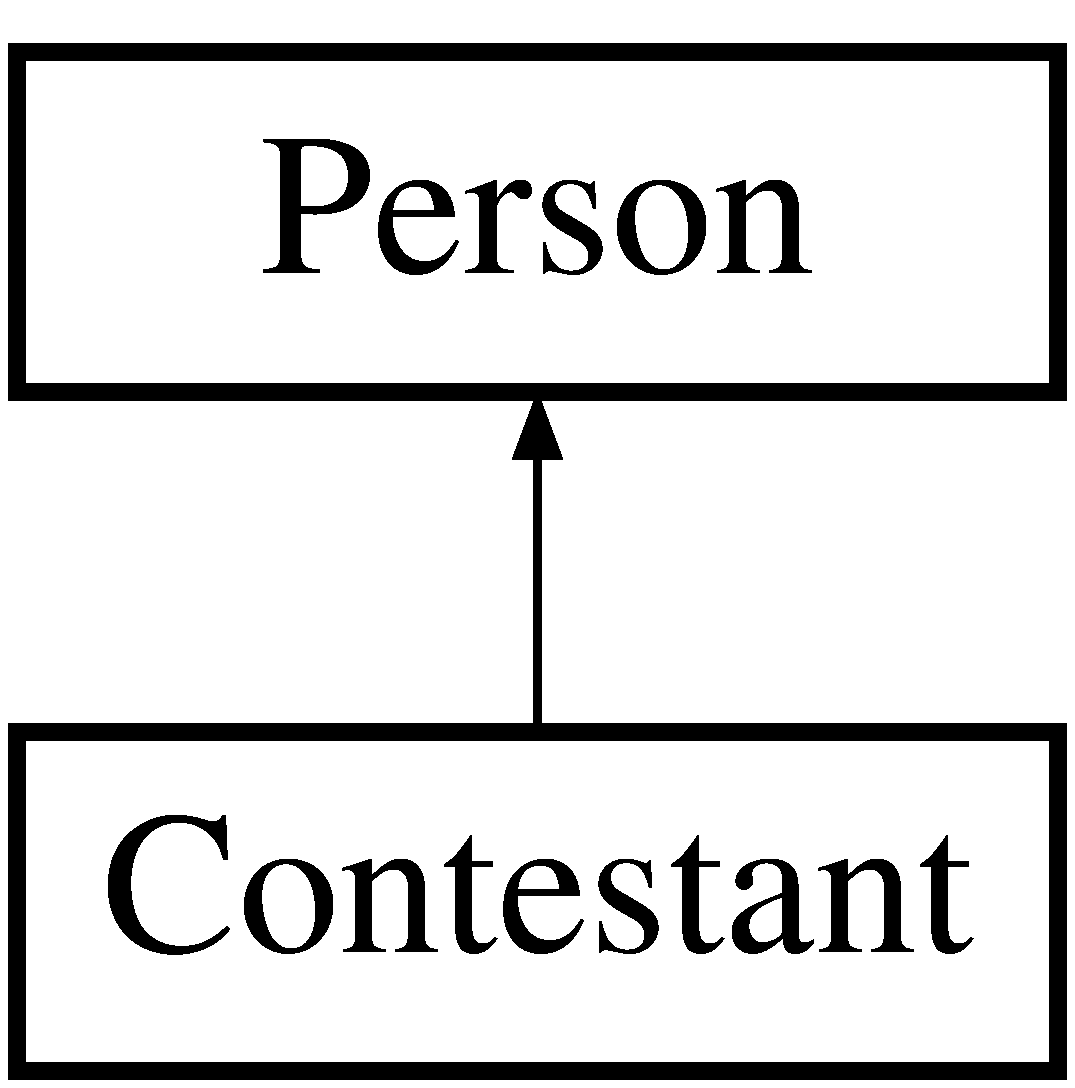
\includegraphics[height=2.000000cm]{class_contestant}
\end{center}
\end{figure}
\subsection*{Public Member Functions}
\begin{DoxyCompactItemize}
\item 
\hyperlink{class_contestant_a4f6ad68b8ea17d3cfc18581f62ea4806}{Contestant} (unsigned int id, std\+::string name, std\+::string address, unsigned int mobile, \hyperlink{class_calendar}{Calendar} dob, std\+::string specialty, std\+::vector$<$ unsigned int $>$ participation)
\begin{DoxyCompactList}\small\item\em \hyperlink{class_contestant}{Contestant} Contructor with their id, name, address, mobile phone number, date of birth, specialiy and list of participations by id. \end{DoxyCompactList}\item 
\hyperlink{class_contestant_ad9d2408c8ffd36832801c25d836be630}{Contestant} (std\+::string text\+Line)
\begin{DoxyCompactList}\small\item\em \hyperlink{class_contestant}{Contestant} Contructor by reading a line from \hyperlink{class_contestant}{Contestant} file. \end{DoxyCompactList}\item 
unsigned int \hyperlink{class_contestant_af3b5ca4f5150092fac946d6aa7301cd3}{get\+Id} () const
\begin{DoxyCompactList}\small\item\em Manages to access the \hyperlink{class_contestant}{Contestant}\textquotesingle{}s ID value. \end{DoxyCompactList}\item 
std\+::vector$<$ \hyperlink{class_participation}{Participation} $\ast$ $>$ \hyperlink{class_contestant_abd0caa85a134d63212cf9e0f9ccc7a1d}{get\+Participations} () const
\begin{DoxyCompactList}\small\item\em Manages to access all participations that the specified \hyperlink{class_contestant}{Contestant} has had. \end{DoxyCompactList}\item 
void \hyperlink{class_contestant_add8973daf90279756d9ba846dcbffa67}{set\+Id} (unsigned int id)
\begin{DoxyCompactList}\small\item\em Changes the ID of a current \hyperlink{class_contestant}{Contestant}. \end{DoxyCompactList}\item 
void \hyperlink{class_contestant_a0ca184f1d5064ad78e7b5f643c8e4f42}{set\+Participations} (std\+::vector$<$ \hyperlink{class_participation}{Participation} $\ast$$>$ participation)
\begin{DoxyCompactList}\small\item\em Changes the participations of a current \hyperlink{class_contestant}{Contestant}. \end{DoxyCompactList}\item 
\mbox{\Hypertarget{class_contestant_a7c89f356696d59b7ccb762d09451def3}\label{class_contestant_a7c89f356696d59b7ccb762d09451def3}} 
void \hyperlink{class_contestant_a7c89f356696d59b7ccb762d09451def3}{show} () const
\begin{DoxyCompactList}\small\item\em Prints the \hyperlink{class_contestant}{Contestant}\textquotesingle{}s full information on the screen. \end{DoxyCompactList}\item 
bool \hyperlink{class_contestant_ae51d0d7eb8a0cf2e70f0cfe92c74e7ae}{operator$<$} (const \hyperlink{class_contestant}{Contestant} \&contestant1) const
\item 
bool \hyperlink{class_contestant_a6d1d627ddf49dc5d3b77a6d42a3680fd}{operator==} (const \hyperlink{class_contestant}{Contestant} \&contestant1) const
\end{DoxyCompactItemize}
\subsection*{Friends}
\begin{DoxyCompactItemize}
\item 
std\+::ostream \& \hyperlink{class_contestant_af6619c3c4998b08f93ea4a4568201ebe}{operator$<$$<$} (std\+::ostream \&os, const \hyperlink{class_contestant}{Contestant} \&contestant)
\end{DoxyCompactItemize}
\subsection*{Additional Inherited Members}


\subsection{Detailed Description}
Project Untitled 

\subsection{Constructor \& Destructor Documentation}
\mbox{\Hypertarget{class_contestant_a4f6ad68b8ea17d3cfc18581f62ea4806}\label{class_contestant_a4f6ad68b8ea17d3cfc18581f62ea4806}} 
\index{Contestant@{Contestant}!Contestant@{Contestant}}
\index{Contestant@{Contestant}!Contestant@{Contestant}}
\subsubsection{\texorpdfstring{Contestant()}{Contestant()}\hspace{0.1cm}{\footnotesize\ttfamily [1/2]}}
{\footnotesize\ttfamily Contestant\+::\+Contestant (\begin{DoxyParamCaption}\item[{unsigned int}]{id,  }\item[{std\+::string}]{name,  }\item[{std\+::string}]{address,  }\item[{unsigned int}]{mobile,  }\item[{\hyperlink{class_calendar}{Calendar}}]{dob,  }\item[{std\+::string}]{specialty,  }\item[{std\+::vector$<$ unsigned int $>$}]{participation }\end{DoxyParamCaption})}



\hyperlink{class_contestant}{Contestant} Contructor with their id, name, address, mobile phone number, date of birth, specialiy and list of participations by id. 


\begin{DoxyParams}{Parameters}
{\em id} & an unsigined integer \\
\hline
{\em name} & a string \\
\hline
{\em address} & a string \\
\hline
{\em mobile} & an unsigined int \\
\hline
{\em dob} & a \hyperlink{class_calendar}{Calendar} Object \\
\hline
{\em specialiy} & a string \\
\hline
{\em participation} & a vector of unsigined int \\
\hline
\end{DoxyParams}
\mbox{\Hypertarget{class_contestant_ad9d2408c8ffd36832801c25d836be630}\label{class_contestant_ad9d2408c8ffd36832801c25d836be630}} 
\index{Contestant@{Contestant}!Contestant@{Contestant}}
\index{Contestant@{Contestant}!Contestant@{Contestant}}
\subsubsection{\texorpdfstring{Contestant()}{Contestant()}\hspace{0.1cm}{\footnotesize\ttfamily [2/2]}}
{\footnotesize\ttfamily Contestant\+::\+Contestant (\begin{DoxyParamCaption}\item[{std\+::string}]{text\+Line }\end{DoxyParamCaption})}



\hyperlink{class_contestant}{Contestant} Contructor by reading a line from \hyperlink{class_contestant}{Contestant} file. 


\begin{DoxyParams}{Parameters}
{\em textline} & as string \\
\hline
\end{DoxyParams}


\subsection{Member Function Documentation}
\mbox{\Hypertarget{class_contestant_af3b5ca4f5150092fac946d6aa7301cd3}\label{class_contestant_af3b5ca4f5150092fac946d6aa7301cd3}} 
\index{Contestant@{Contestant}!get\+Id@{get\+Id}}
\index{get\+Id@{get\+Id}!Contestant@{Contestant}}
\subsubsection{\texorpdfstring{get\+Id()}{getId()}}
{\footnotesize\ttfamily unsigned int Contestant\+::get\+Id (\begin{DoxyParamCaption}{ }\end{DoxyParamCaption}) const}



Manages to access the \hyperlink{class_contestant}{Contestant}\textquotesingle{}s ID value. 

\begin{DoxyReturn}{Returns}
unsigned integer of the \hyperlink{class_contestant}{Contestant}\textquotesingle{}s ID 
\end{DoxyReturn}
\mbox{\Hypertarget{class_contestant_abd0caa85a134d63212cf9e0f9ccc7a1d}\label{class_contestant_abd0caa85a134d63212cf9e0f9ccc7a1d}} 
\index{Contestant@{Contestant}!get\+Participations@{get\+Participations}}
\index{get\+Participations@{get\+Participations}!Contestant@{Contestant}}
\subsubsection{\texorpdfstring{get\+Participations()}{getParticipations()}}
{\footnotesize\ttfamily vector$<$ \hyperlink{class_participation}{Participation} $\ast$ $>$ Contestant\+::get\+Participations (\begin{DoxyParamCaption}{ }\end{DoxyParamCaption}) const}



Manages to access all participations that the specified \hyperlink{class_contestant}{Contestant} has had. 

\begin{DoxyReturn}{Returns}
a contestant vector of participations pointers from the specified \hyperlink{class_contestant}{Contestant} 
\end{DoxyReturn}
\mbox{\Hypertarget{class_contestant_ae51d0d7eb8a0cf2e70f0cfe92c74e7ae}\label{class_contestant_ae51d0d7eb8a0cf2e70f0cfe92c74e7ae}} 
\index{Contestant@{Contestant}!operator$<$@{operator$<$}}
\index{operator$<$@{operator$<$}!Contestant@{Contestant}}
\subsubsection{\texorpdfstring{operator$<$()}{operator<()}}
{\footnotesize\ttfamily bool Contestant\+::operator$<$ (\begin{DoxyParamCaption}\item[{const \hyperlink{class_contestant}{Contestant} \&}]{contestant1 }\end{DoxyParamCaption}) const}

Operator \char`\"{}$<$\char`\"{} is overloaded to compare the ID value of the Object \hyperlink{class_contestant}{Contestant} with a specific \hyperlink{class_contestant}{Contestant} 
\begin{DoxyParams}{Parameters}
{\em contestant1} & a constant \hyperlink{class_contestant}{Contestant} reference \\
\hline
\end{DoxyParams}
\begin{DoxyReturn}{Returns}
true if the Object is greater than contestant1\textquotesingle{}s id and false if the Object is lesser than contestant1\textquotesingle{}s id 
\end{DoxyReturn}
\mbox{\Hypertarget{class_contestant_a6d1d627ddf49dc5d3b77a6d42a3680fd}\label{class_contestant_a6d1d627ddf49dc5d3b77a6d42a3680fd}} 
\index{Contestant@{Contestant}!operator==@{operator==}}
\index{operator==@{operator==}!Contestant@{Contestant}}
\subsubsection{\texorpdfstring{operator==()}{operator==()}}
{\footnotesize\ttfamily bool Contestant\+::operator== (\begin{DoxyParamCaption}\item[{const \hyperlink{class_contestant}{Contestant} \&}]{contestant1 }\end{DoxyParamCaption}) const}

Operator \char`\"{}==\char`\"{} is overloaded to check if the Object \hyperlink{class_contestant}{Contestant} is equal to another given \hyperlink{class_contestant}{Contestant} in case they share the same properties 
\begin{DoxyParams}{Parameters}
{\em contestant1} & a constant \hyperlink{class_contestant}{Contestant} reference \\
\hline
\end{DoxyParams}
\begin{DoxyReturn}{Returns}
true if the Object is equal to contestant1\textquotesingle{}s properties and false if the Object is not equal to contestant1\textquotesingle{}s properties 
\end{DoxyReturn}
\mbox{\Hypertarget{class_contestant_add8973daf90279756d9ba846dcbffa67}\label{class_contestant_add8973daf90279756d9ba846dcbffa67}} 
\index{Contestant@{Contestant}!set\+Id@{set\+Id}}
\index{set\+Id@{set\+Id}!Contestant@{Contestant}}
\subsubsection{\texorpdfstring{set\+Id()}{setId()}}
{\footnotesize\ttfamily void Contestant\+::set\+Id (\begin{DoxyParamCaption}\item[{unsigned int}]{id }\end{DoxyParamCaption})}



Changes the ID of a current \hyperlink{class_contestant}{Contestant}. 


\begin{DoxyParams}{Parameters}
{\em id} & an unsigned integer argument \\
\hline
\end{DoxyParams}
\mbox{\Hypertarget{class_contestant_a0ca184f1d5064ad78e7b5f643c8e4f42}\label{class_contestant_a0ca184f1d5064ad78e7b5f643c8e4f42}} 
\index{Contestant@{Contestant}!set\+Participations@{set\+Participations}}
\index{set\+Participations@{set\+Participations}!Contestant@{Contestant}}
\subsubsection{\texorpdfstring{set\+Participations()}{setParticipations()}}
{\footnotesize\ttfamily void Contestant\+::set\+Participations (\begin{DoxyParamCaption}\item[{std\+::vector$<$ \hyperlink{class_participation}{Participation} $\ast$$>$}]{participation }\end{DoxyParamCaption})}



Changes the participations of a current \hyperlink{class_contestant}{Contestant}. 


\begin{DoxyParams}{Parameters}
{\em participation} & a vector of \hyperlink{class_participation}{Participation} pointers \\
\hline
\end{DoxyParams}


\subsection{Friends And Related Function Documentation}
\mbox{\Hypertarget{class_contestant_af6619c3c4998b08f93ea4a4568201ebe}\label{class_contestant_af6619c3c4998b08f93ea4a4568201ebe}} 
\index{Contestant@{Contestant}!operator$<$$<$@{operator$<$$<$}}
\index{operator$<$$<$@{operator$<$$<$}!Contestant@{Contestant}}
\subsubsection{\texorpdfstring{operator$<$$<$}{operator<<}}
{\footnotesize\ttfamily std\+::ostream\& operator$<$$<$ (\begin{DoxyParamCaption}\item[{std\+::ostream \&}]{os,  }\item[{const \hyperlink{class_contestant}{Contestant} \&}]{contestant }\end{DoxyParamCaption})\hspace{0.3cm}{\ttfamily [friend]}}

Operator \char`\"{}$<$$<$\char`\"{} is overloaded to output the information about the \hyperlink{class_contestant}{Contestant} into a file 
\begin{DoxyParams}{Parameters}
{\em contestant1} & a constant \hyperlink{class_contestant}{Contestant} reference \\
\hline
\end{DoxyParams}
\begin{DoxyReturn}{Returns}
ostream reference of the information of the contestant in a specific format into a file 
\end{DoxyReturn}


The documentation for this class was generated from the following files\+:\begin{DoxyCompactItemize}
\item 
Contestant.\+h\item 
Contestant.\+cpp\end{DoxyCompactItemize}

\hypertarget{class_contestant_id_not_found}{}\section{Contestant\+Id\+Not\+Found Class Reference}
\label{class_contestant_id_not_found}\index{Contestant\+Id\+Not\+Found@{Contestant\+Id\+Not\+Found}}
\subsection*{Public Member Functions}
\begin{DoxyCompactItemize}
\item 
\mbox{\Hypertarget{class_contestant_id_not_found_a6496870d812f16d0b1fa14a656bb0970}\label{class_contestant_id_not_found_a6496870d812f16d0b1fa14a656bb0970}} 
{\bfseries Contestant\+Id\+Not\+Found} (unsigned int id)
\item 
unsigned int \hyperlink{class_contestant_id_not_found_a99fe92bc67ebb5c44bb1f3dc28dc52cb}{get\+Id} () const
\begin{DoxyCompactList}\small\item\em Manages to get the id of the contestant that was not found. \end{DoxyCompactList}\end{DoxyCompactItemize}


\subsection{Member Function Documentation}
\mbox{\Hypertarget{class_contestant_id_not_found_a99fe92bc67ebb5c44bb1f3dc28dc52cb}\label{class_contestant_id_not_found_a99fe92bc67ebb5c44bb1f3dc28dc52cb}} 
\index{Contestant\+Id\+Not\+Found@{Contestant\+Id\+Not\+Found}!get\+Id@{get\+Id}}
\index{get\+Id@{get\+Id}!Contestant\+Id\+Not\+Found@{Contestant\+Id\+Not\+Found}}
\subsubsection{\texorpdfstring{get\+Id()}{getId()}}
{\footnotesize\ttfamily unsigned int Contestant\+Id\+Not\+Found\+::get\+Id (\begin{DoxyParamCaption}{ }\end{DoxyParamCaption}) const\hspace{0.3cm}{\ttfamily [inline]}}



Manages to get the id of the contestant that was not found. 

\begin{DoxyReturn}{Returns}
unsigned integer id of the contestant not found 
\end{DoxyReturn}


The documentation for this class was generated from the following file\+:\begin{DoxyCompactItemize}
\item 
Exception\+Hand.\+h\end{DoxyCompactItemize}

\hypertarget{class_contestant_info_not_found}{}\section{Contestant\+Info\+Not\+Found Class Reference}
\label{class_contestant_info_not_found}\index{Contestant\+Info\+Not\+Found@{Contestant\+Info\+Not\+Found}}


The documentation for this class was generated from the following file\+:\begin{DoxyCompactItemize}
\item 
Exception\+Hand.\+h\end{DoxyCompactItemize}

\hypertarget{class_empty_answer}{}\section{Empty\+Answer Class Reference}
\label{class_empty_answer}\index{Empty\+Answer@{Empty\+Answer}}


The documentation for this class was generated from the following file\+:\begin{DoxyCompactItemize}
\item 
Exception\+Hand.\+h\end{DoxyCompactItemize}

\hypertarget{class_first_phase}{}\section{First\+Phase Class Reference}
\label{class_first_phase}\index{First\+Phase@{First\+Phase}}


{\ttfamily \#include $<$First\+Phase.\+h$>$}

Inheritance diagram for First\+Phase\+:\begin{figure}[H]
\begin{center}
\leavevmode
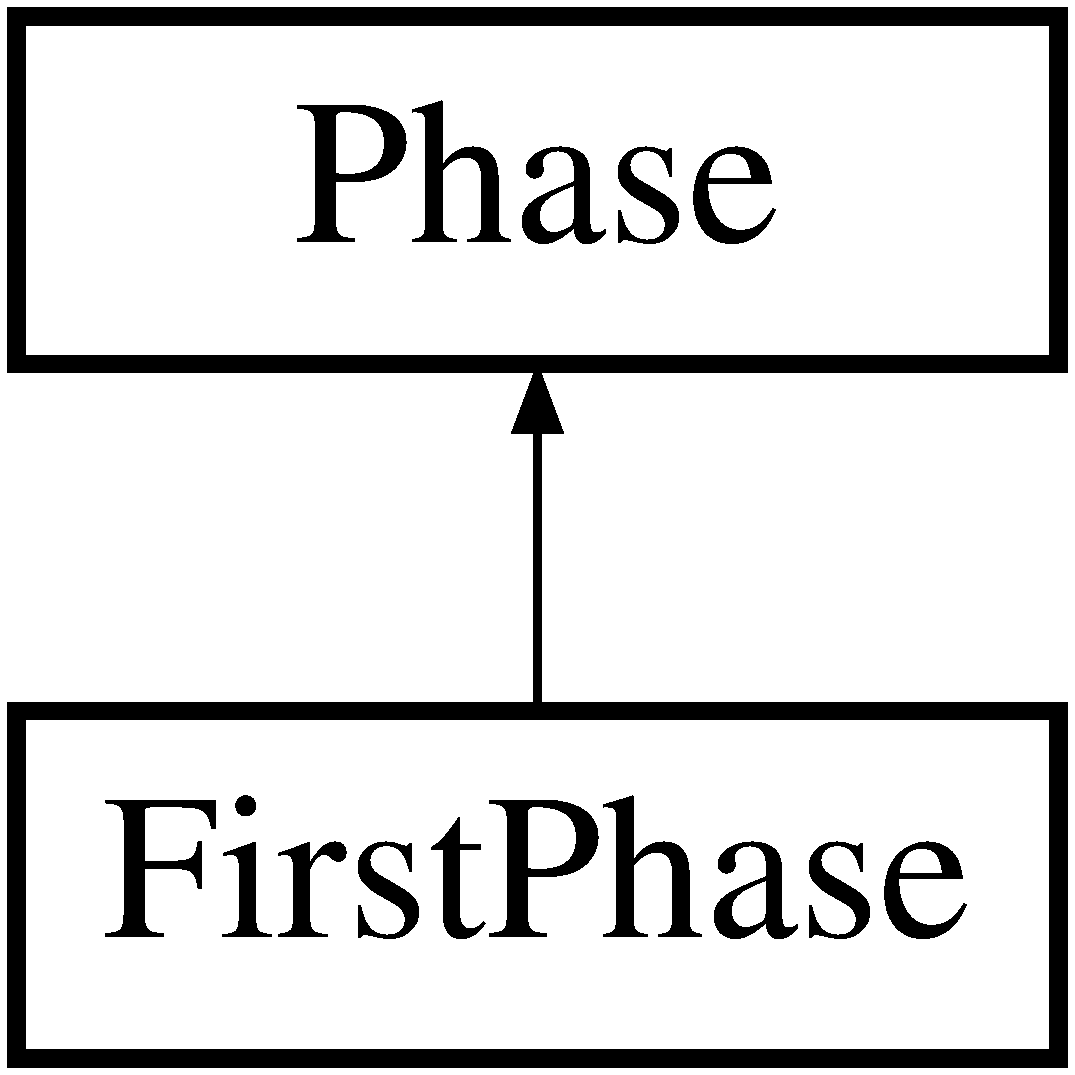
\includegraphics[height=2.000000cm]{class_first_phase}
\end{center}
\end{figure}
\subsection*{Public Member Functions}
\begin{DoxyCompactItemize}
\item 
\mbox{\Hypertarget{class_first_phase_a1e392056f4bdc298e75eed593862561d}\label{class_first_phase_a1e392056f4bdc298e75eed593862561d}} 
\hyperlink{class_first_phase_a1e392056f4bdc298e75eed593862561d}{First\+Phase} ()
\begin{DoxyCompactList}\small\item\em First \hyperlink{class_phase}{Phase} default constructor. \end{DoxyCompactList}\item 
\mbox{\Hypertarget{class_first_phase_a7ba9ba5a957ae942c52d9d0c27de3391}\label{class_first_phase_a7ba9ba5a957ae942c52d9d0c27de3391}} 
\hyperlink{class_first_phase_a7ba9ba5a957ae942c52d9d0c27de3391}{$\sim$\+First\+Phase} ()
\begin{DoxyCompactList}\small\item\em First \hyperlink{class_phase}{Phase} deconstructor. \end{DoxyCompactList}\item 
\hyperlink{class_first_phase_a1c8d914b5b30eff510d884cc4ab699d6}{First\+Phase} (unsigned int audition\+Id, std\+::vector$<$ unsigned int $>$ final\+\_\+grade, std\+::vector$<$ unsigned int $>$ ev1, std\+::vector$<$ unsigned int $>$ ev2, std\+::vector$<$ unsigned int $>$ ld, std\+::vector$<$ unsigned int $>$ contestants)
\begin{DoxyCompactList}\small\item\em First \hyperlink{class_phase}{Phase} default constructor with their audition\+ID, final grade, evaluation from the judges and the id of the contestants. \end{DoxyCompactList}\item 
\hyperlink{class_first_phase_a2b8412b1a684c1415841c43950701d01}{First\+Phase} (std\+::string textline)
\begin{DoxyCompactList}\small\item\em First \hyperlink{class_phase}{Phase} constructor by reading a line from the file. \end{DoxyCompactList}\item 
\mbox{\Hypertarget{class_first_phase_a89e84246611eaed02077e9c0baccac73}\label{class_first_phase_a89e84246611eaed02077e9c0baccac73}} 
void \hyperlink{class_first_phase_a89e84246611eaed02077e9c0baccac73}{overall\+Grading} ()
\begin{DoxyCompactList}\small\item\em Grades all contestants from the second phase. \end{DoxyCompactList}\end{DoxyCompactItemize}
\subsection*{Friends}
\begin{DoxyCompactItemize}
\item 
std\+::ostream \& \hyperlink{class_first_phase_a402f79e6ed4dcdeaf9745b245ff1b375}{operator$<$$<$} (std\+::ostream \&os, const \hyperlink{class_first_phase}{First\+Phase} \&first\+Phase)
\begin{DoxyCompactList}\small\item\em Operator \char`\"{}$<$$<$\char`\"{} is overloaded to output the information about the First \hyperlink{class_phase}{Phase} into a file. \end{DoxyCompactList}\end{DoxyCompactItemize}
\subsection*{Additional Inherited Members}


\subsection{Detailed Description}
Project Untitled 

\subsection{Constructor \& Destructor Documentation}
\mbox{\Hypertarget{class_first_phase_a1c8d914b5b30eff510d884cc4ab699d6}\label{class_first_phase_a1c8d914b5b30eff510d884cc4ab699d6}} 
\index{First\+Phase@{First\+Phase}!First\+Phase@{First\+Phase}}
\index{First\+Phase@{First\+Phase}!First\+Phase@{First\+Phase}}
\subsubsection{\texorpdfstring{First\+Phase()}{FirstPhase()}\hspace{0.1cm}{\footnotesize\ttfamily [1/2]}}
{\footnotesize\ttfamily First\+Phase\+::\+First\+Phase (\begin{DoxyParamCaption}\item[{unsigned int}]{audition\+Id,  }\item[{std\+::vector$<$ unsigned int $>$}]{final\+\_\+grade,  }\item[{std\+::vector$<$ unsigned int $>$}]{ev1,  }\item[{std\+::vector$<$ unsigned int $>$}]{ev2,  }\item[{std\+::vector$<$ unsigned int $>$}]{ld,  }\item[{std\+::vector$<$ unsigned int $>$}]{contestants }\end{DoxyParamCaption})}



First \hyperlink{class_phase}{Phase} default constructor with their audition\+ID, final grade, evaluation from the judges and the id of the contestants. 


\begin{DoxyParams}{Parameters}
{\em audition\+ID} & an unsigned integer \\
\hline
{\em final\+\_\+grade} & a vector of unsigned integers \\
\hline
{\em ev1} & a vector of unsigned integers \\
\hline
{\em ev2} & a vector of unsigned integers \\
\hline
{\em ld} & a vector of unsigned integers \\
\hline
{\em contestants} & a vector of unsigned integers \\
\hline
\end{DoxyParams}
\mbox{\Hypertarget{class_first_phase_a2b8412b1a684c1415841c43950701d01}\label{class_first_phase_a2b8412b1a684c1415841c43950701d01}} 
\index{First\+Phase@{First\+Phase}!First\+Phase@{First\+Phase}}
\index{First\+Phase@{First\+Phase}!First\+Phase@{First\+Phase}}
\subsubsection{\texorpdfstring{First\+Phase()}{FirstPhase()}\hspace{0.1cm}{\footnotesize\ttfamily [2/2]}}
{\footnotesize\ttfamily First\+Phase\+::\+First\+Phase (\begin{DoxyParamCaption}\item[{std\+::string}]{textline }\end{DoxyParamCaption})}



First \hyperlink{class_phase}{Phase} constructor by reading a line from the file. 


\begin{DoxyParams}{Parameters}
{\em text\+Line} & a string \\
\hline
\end{DoxyParams}


\subsection{Friends And Related Function Documentation}
\mbox{\Hypertarget{class_first_phase_a402f79e6ed4dcdeaf9745b245ff1b375}\label{class_first_phase_a402f79e6ed4dcdeaf9745b245ff1b375}} 
\index{First\+Phase@{First\+Phase}!operator$<$$<$@{operator$<$$<$}}
\index{operator$<$$<$@{operator$<$$<$}!First\+Phase@{First\+Phase}}
\subsubsection{\texorpdfstring{operator$<$$<$}{operator<<}}
{\footnotesize\ttfamily std\+::ostream\& operator$<$$<$ (\begin{DoxyParamCaption}\item[{std\+::ostream \&}]{os,  }\item[{const \hyperlink{class_first_phase}{First\+Phase} \&}]{first\+Phase }\end{DoxyParamCaption})\hspace{0.3cm}{\ttfamily [friend]}}



Operator \char`\"{}$<$$<$\char`\"{} is overloaded to output the information about the First \hyperlink{class_phase}{Phase} into a file. 


\begin{DoxyParams}{Parameters}
{\em os} & an Outstream Object \\
\hline
{\em first\+Phase} & a constant \hyperlink{class_first_phase}{First\+Phase} reference \\
\hline
\end{DoxyParams}
\begin{DoxyReturn}{Returns}
ostream reference of the information of the First \hyperlink{class_phase}{Phase} in a specific format into a file 
\end{DoxyReturn}


The documentation for this class was generated from the following files\+:\begin{DoxyCompactItemize}
\item 
First\+Phase.\+h\item 
First\+Phase.\+cpp\end{DoxyCompactItemize}

\hypertarget{class_invalid_id}{}\section{Invalid\+Id Class Reference}
\label{class_invalid_id}\index{Invalid\+Id@{Invalid\+Id}}


The documentation for this class was generated from the following file\+:\begin{DoxyCompactItemize}
\item 
Exception\+Hand.\+h\end{DoxyCompactItemize}

\hypertarget{class_invalid_option}{}\section{Invalid\+Option Class Reference}
\label{class_invalid_option}\index{Invalid\+Option@{Invalid\+Option}}


The documentation for this class was generated from the following file\+:\begin{DoxyCompactItemize}
\item 
Exception\+Hand.\+h\end{DoxyCompactItemize}

\hypertarget{class_judge}{}\section{Judge Class Reference}
\label{class_judge}\index{Judge@{Judge}}
Inheritance diagram for Judge\+:\begin{figure}[H]
\begin{center}
\leavevmode
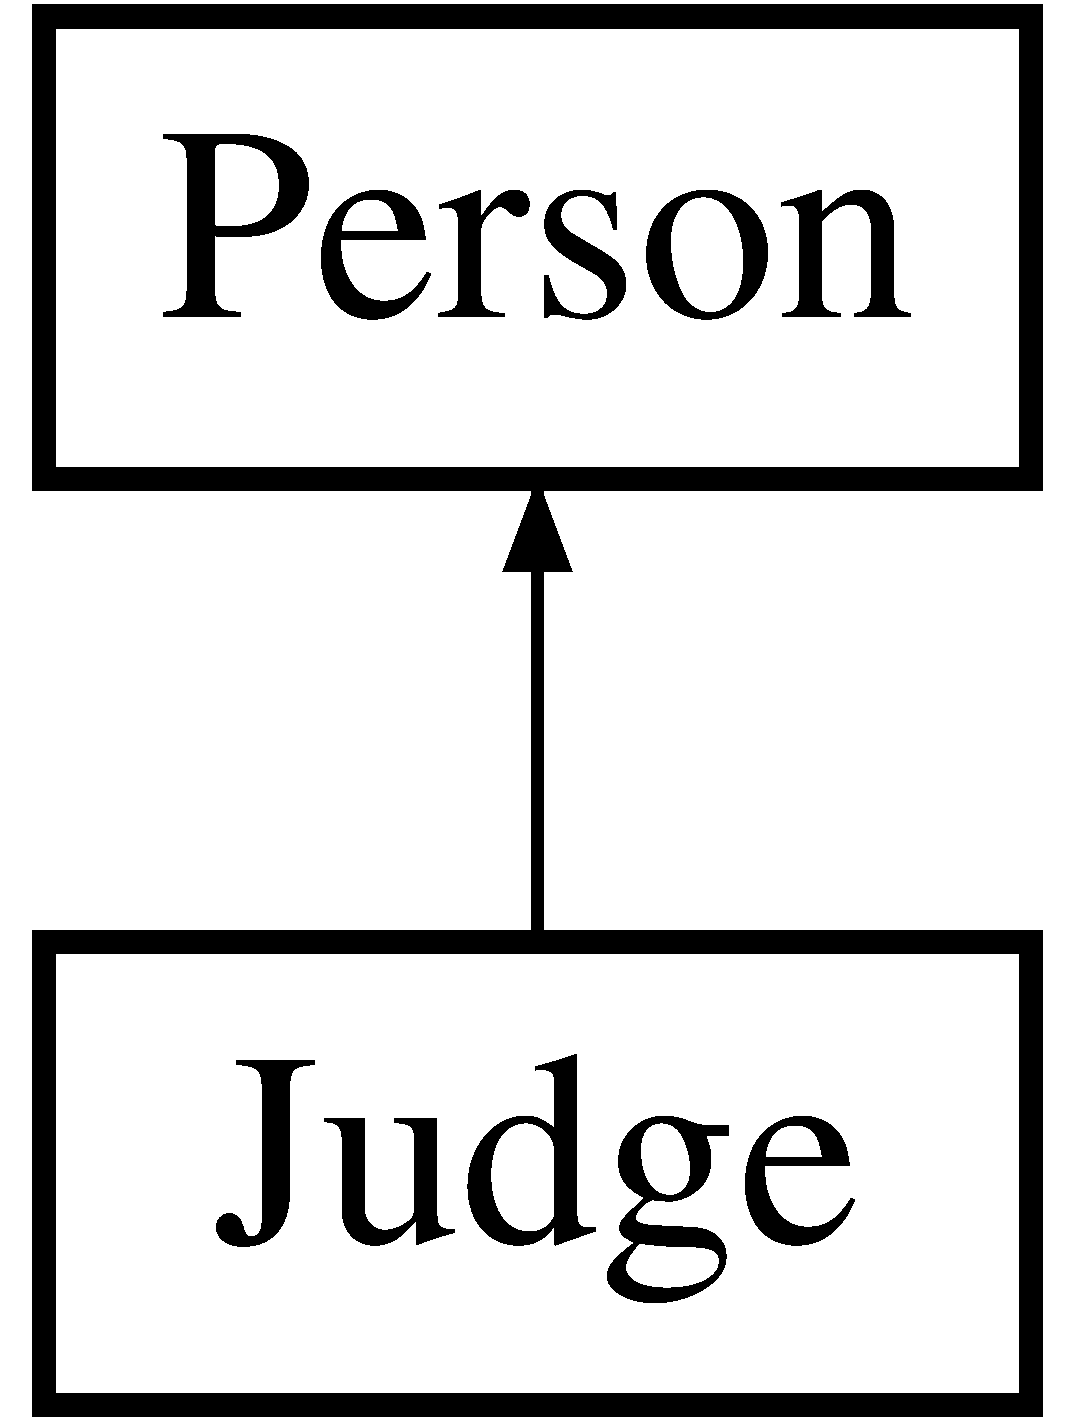
\includegraphics[height=2.000000cm]{class_judge}
\end{center}
\end{figure}
\subsection*{Public Member Functions}
\begin{DoxyCompactItemize}
\item 
\mbox{\Hypertarget{class_judge_a76a14e0c72af67cb72152b6f176111cf}\label{class_judge_a76a14e0c72af67cb72152b6f176111cf}} 
\hyperlink{class_judge_a76a14e0c72af67cb72152b6f176111cf}{Judge} ()
\begin{DoxyCompactList}\small\item\em \hyperlink{class_judge}{Judge} Default Contructor. \end{DoxyCompactList}\item 
\hyperlink{class_judge_ad8e4c64a5b1cb72fc4f1f907117d97c3}{Judge} (unsigned int id, std\+::string name, std\+::string address, unsigned int mobile, \hyperlink{class_calendar}{Calendar} dob, std\+::string specialty, std\+::vector$<$ unsigned int $>$ participation)
\begin{DoxyCompactList}\small\item\em \hyperlink{class_judge}{Judge} Contructor with their id, name, address, mobile phone number, date of birth, specialiy and list of participations by id. \end{DoxyCompactList}\item 
\hyperlink{class_judge_a50775ff3e2a60d6c12893790e195a97e}{Judge} (std\+::string textline)
\begin{DoxyCompactList}\small\item\em \hyperlink{class_judge}{Judge} Contructor by reading a line from \hyperlink{class_judge}{Judge} file. \end{DoxyCompactList}\item 
unsigned int \hyperlink{class_judge_a1db442ff16710223a937fbeb7784c576}{get\+Id} () const
\begin{DoxyCompactList}\small\item\em Manages to access the \hyperlink{class_judge}{Judge}\textquotesingle{}s ID value. \end{DoxyCompactList}\item 
std\+::vector$<$ unsigned int $>$ \hyperlink{class_judge_aa854dfe7153ff301cba9319caeb3599c}{get\+Participations} () const
\begin{DoxyCompactList}\small\item\em Manages to access all participations that the specified \hyperlink{class_judge}{Judge} has had. \end{DoxyCompactList}\item 
void \hyperlink{class_judge_a06f4e2a65994b0e0a2e6aad38af0edea}{set\+Id} (unsigned int id)
\begin{DoxyCompactList}\small\item\em Changes \hyperlink{class_judge}{Judge}\textquotesingle{}s ID. \end{DoxyCompactList}\item 
void \hyperlink{class_judge_ab6bf287475108075c5c95f3fa0d7e6b0}{set\+Participations} (std\+::vector$<$ unsigned int $>$ participation)
\begin{DoxyCompactList}\small\item\em Changes the participations the judge was in. \end{DoxyCompactList}\item 
bool \hyperlink{class_judge_a748c3fae9d2a6cea4952d31ebe2bb660}{operator$<$} (const \hyperlink{class_judge}{Judge} \&judge1) const
\begin{DoxyCompactList}\small\item\em Operator \char`\"{}$<$\char`\"{} is overloaded to compare the ID value of the Object with a specific \hyperlink{class_judge}{Judge}. \end{DoxyCompactList}\item 
bool \hyperlink{class_judge_ab3a06af6dc3a2f5f427c146e2b1a4573}{operator==} (const \hyperlink{class_judge}{Judge} \&judge1) const
\item 
\mbox{\Hypertarget{class_judge_a54d7671b2a8d4fb249378914c9ae1746}\label{class_judge_a54d7671b2a8d4fb249378914c9ae1746}} 
void \hyperlink{class_judge_a54d7671b2a8d4fb249378914c9ae1746}{show} ()
\begin{DoxyCompactList}\small\item\em Prints the \hyperlink{class_judge}{Judge}\textquotesingle{}s full information on the screen. \end{DoxyCompactList}\end{DoxyCompactItemize}
\subsection*{Friends}
\begin{DoxyCompactItemize}
\item 
std\+::ostream \& \hyperlink{class_judge_ad83f9941c7a7e0ae112d4fcf186f86cb}{operator$<$$<$} (std\+::ostream \&os, const \hyperlink{class_judge}{Judge} \&judge)
\end{DoxyCompactItemize}
\subsection*{Additional Inherited Members}


\subsection{Constructor \& Destructor Documentation}
\mbox{\Hypertarget{class_judge_ad8e4c64a5b1cb72fc4f1f907117d97c3}\label{class_judge_ad8e4c64a5b1cb72fc4f1f907117d97c3}} 
\index{Judge@{Judge}!Judge@{Judge}}
\index{Judge@{Judge}!Judge@{Judge}}
\subsubsection{\texorpdfstring{Judge()}{Judge()}\hspace{0.1cm}{\footnotesize\ttfamily [1/2]}}
{\footnotesize\ttfamily Judge\+::\+Judge (\begin{DoxyParamCaption}\item[{unsigned int}]{id,  }\item[{std\+::string}]{name,  }\item[{std\+::string}]{address,  }\item[{unsigned int}]{mobile,  }\item[{\hyperlink{class_calendar}{Calendar}}]{dob,  }\item[{std\+::string}]{specialty,  }\item[{std\+::vector$<$ unsigned int $>$}]{participation }\end{DoxyParamCaption})}



\hyperlink{class_judge}{Judge} Contructor with their id, name, address, mobile phone number, date of birth, specialiy and list of participations by id. 


\begin{DoxyParams}{Parameters}
{\em id} & an unsigined integer \\
\hline
{\em name} & a string \\
\hline
{\em address} & a string \\
\hline
{\em mobile} & an unsigined integer \\
\hline
{\em dob} & a \hyperlink{class_calendar}{Calendar} Object \\
\hline
{\em specialiy} & a string \\
\hline
{\em participation} & a vector of unsigined integer \\
\hline
\end{DoxyParams}
\mbox{\Hypertarget{class_judge_a50775ff3e2a60d6c12893790e195a97e}\label{class_judge_a50775ff3e2a60d6c12893790e195a97e}} 
\index{Judge@{Judge}!Judge@{Judge}}
\index{Judge@{Judge}!Judge@{Judge}}
\subsubsection{\texorpdfstring{Judge()}{Judge()}\hspace{0.1cm}{\footnotesize\ttfamily [2/2]}}
{\footnotesize\ttfamily Judge\+::\+Judge (\begin{DoxyParamCaption}\item[{std\+::string}]{textline }\end{DoxyParamCaption})}



\hyperlink{class_judge}{Judge} Contructor by reading a line from \hyperlink{class_judge}{Judge} file. 


\begin{DoxyParams}{Parameters}
{\em textline} & a string \\
\hline
\end{DoxyParams}


\subsection{Member Function Documentation}
\mbox{\Hypertarget{class_judge_a1db442ff16710223a937fbeb7784c576}\label{class_judge_a1db442ff16710223a937fbeb7784c576}} 
\index{Judge@{Judge}!get\+Id@{get\+Id}}
\index{get\+Id@{get\+Id}!Judge@{Judge}}
\subsubsection{\texorpdfstring{get\+Id()}{getId()}}
{\footnotesize\ttfamily unsigned int Judge\+::get\+Id (\begin{DoxyParamCaption}{ }\end{DoxyParamCaption}) const}



Manages to access the \hyperlink{class_judge}{Judge}\textquotesingle{}s ID value. 

\begin{DoxyReturn}{Returns}
\hyperlink{class_judge}{Judge}\textquotesingle{}s ID 
\end{DoxyReturn}
\mbox{\Hypertarget{class_judge_aa854dfe7153ff301cba9319caeb3599c}\label{class_judge_aa854dfe7153ff301cba9319caeb3599c}} 
\index{Judge@{Judge}!get\+Participations@{get\+Participations}}
\index{get\+Participations@{get\+Participations}!Judge@{Judge}}
\subsubsection{\texorpdfstring{get\+Participations()}{getParticipations()}}
{\footnotesize\ttfamily vector$<$ unsigned int $>$ Judge\+::get\+Participations (\begin{DoxyParamCaption}{ }\end{DoxyParamCaption}) const}



Manages to access all participations that the specified \hyperlink{class_judge}{Judge} has had. 

\begin{DoxyReturn}{Returns}
a constant vector of participations from the specified \hyperlink{class_judge}{Judge} 
\end{DoxyReturn}
\mbox{\Hypertarget{class_judge_a748c3fae9d2a6cea4952d31ebe2bb660}\label{class_judge_a748c3fae9d2a6cea4952d31ebe2bb660}} 
\index{Judge@{Judge}!operator$<$@{operator$<$}}
\index{operator$<$@{operator$<$}!Judge@{Judge}}
\subsubsection{\texorpdfstring{operator$<$()}{operator<()}}
{\footnotesize\ttfamily bool Judge\+::operator$<$ (\begin{DoxyParamCaption}\item[{const \hyperlink{class_judge}{Judge} \&}]{judge1 }\end{DoxyParamCaption}) const}



Operator \char`\"{}$<$\char`\"{} is overloaded to compare the ID value of the Object with a specific \hyperlink{class_judge}{Judge}. 


\begin{DoxyParams}{Parameters}
{\em judge1} & a constant \hyperlink{class_judge}{Judge} reference \\
\hline
\end{DoxyParams}
\begin{DoxyReturn}{Returns}
true if the Object is greater than judge1 and false if the Object is lesser than judge1 
\end{DoxyReturn}
\mbox{\Hypertarget{class_judge_ab3a06af6dc3a2f5f427c146e2b1a4573}\label{class_judge_ab3a06af6dc3a2f5f427c146e2b1a4573}} 
\index{Judge@{Judge}!operator==@{operator==}}
\index{operator==@{operator==}!Judge@{Judge}}
\subsubsection{\texorpdfstring{operator==()}{operator==()}}
{\footnotesize\ttfamily bool Judge\+::operator== (\begin{DoxyParamCaption}\item[{const \hyperlink{class_judge}{Judge} \&}]{judge1 }\end{DoxyParamCaption}) const}

Operator \char`\"{}==\char`\"{} is overloaded to check if the Object \hyperlink{class_judge}{Judge} is equal to another given \hyperlink{class_judge}{Judge} in case they share the same properties 
\begin{DoxyParams}{Parameters}
{\em judge1} & a constant \hyperlink{class_judge}{Judge} reference \\
\hline
\end{DoxyParams}
\begin{DoxyReturn}{Returns}
true if the Object is equal to judge1\textquotesingle{}s properties and false if the Object is not equal to judge1\textquotesingle{}s properties 
\end{DoxyReturn}
\mbox{\Hypertarget{class_judge_a06f4e2a65994b0e0a2e6aad38af0edea}\label{class_judge_a06f4e2a65994b0e0a2e6aad38af0edea}} 
\index{Judge@{Judge}!set\+Id@{set\+Id}}
\index{set\+Id@{set\+Id}!Judge@{Judge}}
\subsubsection{\texorpdfstring{set\+Id()}{setId()}}
{\footnotesize\ttfamily void Judge\+::set\+Id (\begin{DoxyParamCaption}\item[{unsigned int}]{id }\end{DoxyParamCaption})}



Changes \hyperlink{class_judge}{Judge}\textquotesingle{}s ID. 


\begin{DoxyParams}{Parameters}
{\em id} & an unsigined integers \\
\hline
\end{DoxyParams}
\mbox{\Hypertarget{class_judge_ab6bf287475108075c5c95f3fa0d7e6b0}\label{class_judge_ab6bf287475108075c5c95f3fa0d7e6b0}} 
\index{Judge@{Judge}!set\+Participations@{set\+Participations}}
\index{set\+Participations@{set\+Participations}!Judge@{Judge}}
\subsubsection{\texorpdfstring{set\+Participations()}{setParticipations()}}
{\footnotesize\ttfamily void Judge\+::set\+Participations (\begin{DoxyParamCaption}\item[{std\+::vector$<$ unsigned int $>$}]{participation }\end{DoxyParamCaption})}



Changes the participations the judge was in. 


\begin{DoxyParams}{Parameters}
{\em participation} & a vector of unsigined integers \\
\hline
\end{DoxyParams}


\subsection{Friends And Related Function Documentation}
\mbox{\Hypertarget{class_judge_ad83f9941c7a7e0ae112d4fcf186f86cb}\label{class_judge_ad83f9941c7a7e0ae112d4fcf186f86cb}} 
\index{Judge@{Judge}!operator$<$$<$@{operator$<$$<$}}
\index{operator$<$$<$@{operator$<$$<$}!Judge@{Judge}}
\subsubsection{\texorpdfstring{operator$<$$<$}{operator<<}}
{\footnotesize\ttfamily std\+::ostream\& operator$<$$<$ (\begin{DoxyParamCaption}\item[{std\+::ostream \&}]{os,  }\item[{const \hyperlink{class_judge}{Judge} \&}]{judge }\end{DoxyParamCaption})\hspace{0.3cm}{\ttfamily [friend]}}

Operator \char`\"{}$<$$<$\char`\"{} is overloaded to output the information about the \hyperlink{class_judge}{Judge} into a file 
\begin{DoxyParams}{Parameters}
{\em os} & an Output Stream Object referece \\
\hline
{\em judge} & a constant \hyperlink{class_judge}{Judge} reference \\
\hline
\end{DoxyParams}
\begin{DoxyReturn}{Returns}
ostream reference 
\end{DoxyReturn}


The documentation for this class was generated from the following files\+:\begin{DoxyCompactItemize}
\item 
Judge.\+h\item 
Judge.\+cpp\end{DoxyCompactItemize}

\hypertarget{class_judge_id_not_found}{}\section{Judge\+Id\+Not\+Found Class Reference}
\label{class_judge_id_not_found}\index{Judge\+Id\+Not\+Found@{Judge\+Id\+Not\+Found}}
\subsection*{Public Member Functions}
\begin{DoxyCompactItemize}
\item 
\mbox{\Hypertarget{class_judge_id_not_found_a212c1373e661a9da9758fe2291bdc3c7}\label{class_judge_id_not_found_a212c1373e661a9da9758fe2291bdc3c7}} 
{\bfseries Judge\+Id\+Not\+Found} (unsigned int id)
\item 
unsigned int \hyperlink{class_judge_id_not_found_afbc8200e1b1ba44cfe5aa97972eb67fd}{get\+Id} () const
\begin{DoxyCompactList}\small\item\em Manages to get the id of the judge that was not found. \end{DoxyCompactList}\end{DoxyCompactItemize}


\subsection{Member Function Documentation}
\mbox{\Hypertarget{class_judge_id_not_found_afbc8200e1b1ba44cfe5aa97972eb67fd}\label{class_judge_id_not_found_afbc8200e1b1ba44cfe5aa97972eb67fd}} 
\index{Judge\+Id\+Not\+Found@{Judge\+Id\+Not\+Found}!get\+Id@{get\+Id}}
\index{get\+Id@{get\+Id}!Judge\+Id\+Not\+Found@{Judge\+Id\+Not\+Found}}
\subsubsection{\texorpdfstring{get\+Id()}{getId()}}
{\footnotesize\ttfamily unsigned int Judge\+Id\+Not\+Found\+::get\+Id (\begin{DoxyParamCaption}{ }\end{DoxyParamCaption}) const\hspace{0.3cm}{\ttfamily [inline]}}



Manages to get the id of the judge that was not found. 

\begin{DoxyReturn}{Returns}
unsigned integer id of the judge not found 
\end{DoxyReturn}


The documentation for this class was generated from the following file\+:\begin{DoxyCompactItemize}
\item 
Exception\+Hand.\+h\end{DoxyCompactItemize}

\hypertarget{class_judge_info_not_found}{}\section{Judge\+Info\+Not\+Found Class Reference}
\label{class_judge_info_not_found}\index{Judge\+Info\+Not\+Found@{Judge\+Info\+Not\+Found}}


The documentation for this class was generated from the following file\+:\begin{DoxyCompactItemize}
\item 
Exception\+Hand.\+h\end{DoxyCompactItemize}

\hypertarget{class_not_a_number}{}\section{Not\+A\+Number Class Reference}
\label{class_not_a_number}\index{Not\+A\+Number@{Not\+A\+Number}}


The documentation for this class was generated from the following file\+:\begin{DoxyCompactItemize}
\item 
Exception\+Hand.\+h\end{DoxyCompactItemize}

\hypertarget{class_not_yes_or_no}{}\section{Not\+Yes\+Or\+No Class Reference}
\label{class_not_yes_or_no}\index{Not\+Yes\+Or\+No@{Not\+Yes\+Or\+No}}


The documentation for this class was generated from the following file\+:\begin{DoxyCompactItemize}
\item 
Exception\+Hand.\+h\end{DoxyCompactItemize}

\hypertarget{class_option_out_of_range}{}\section{Option\+Out\+Of\+Range Class Reference}
\label{class_option_out_of_range}\index{Option\+Out\+Of\+Range@{Option\+Out\+Of\+Range}}


The documentation for this class was generated from the following file\+:\begin{DoxyCompactItemize}
\item 
Exception\+Hand.\+h\end{DoxyCompactItemize}

\hypertarget{class_participation}{}\section{Participation Class Reference}
\label{class_participation}\index{Participation@{Participation}}
\subsection*{Public Member Functions}
\begin{DoxyCompactItemize}
\item 
\hyperlink{class_participation_a7007df223dc88b9bd9a43f0b9d46d4f4}{Participation} (unsigned int audition\+Id, unsigned int place, unsigned int chief\+Judge\+Grade)
\begin{DoxyCompactList}\small\item\em \hyperlink{class_participation}{Participation} Contructor with their audition id, place and the resposible judge\textquotesingle{}s grade. \end{DoxyCompactList}\item 
unsigned int \hyperlink{class_participation_aede9a8356da23d9ee7f4c9c422a05945}{get\+Audition\+Id} () const
\begin{DoxyCompactList}\small\item\em Manages to access the \hyperlink{class_audition}{Audition}\textquotesingle{}s ID the contestant was in. \end{DoxyCompactList}\item 
unsigned int \hyperlink{class_participation_a67add733b1f6fe05b47ebd883486cb3c}{get\+Place} () const
\begin{DoxyCompactList}\small\item\em Manages to access the ranking the contestant got. \end{DoxyCompactList}\item 
unsigned int \hyperlink{class_participation_ad13c6d16677eefc0fb304b074bff97f6}{get\+Chied\+Judge\+Grade} () const
\begin{DoxyCompactList}\small\item\em Manages to access the value that the responsible judge grade the contestant. \end{DoxyCompactList}\item 
void \hyperlink{class_participation_a0cbd915372021b71926187605f94b386}{set\+Audition\+Id} (unsigned int audition\+Id)
\begin{DoxyCompactList}\small\item\em Changes the audition\textquotesingle{}s id. \end{DoxyCompactList}\item 
void \hyperlink{class_participation_a845f29c1f89a79783e2e93b281dc5846}{set\+Place} (unsigned int place)
\begin{DoxyCompactList}\small\item\em Changes the contestant\textquotesingle{}s ranking. \end{DoxyCompactList}\item 
void \hyperlink{class_participation_ad53339e32a85fb8b38f15ee5604e952b}{set\+Chief\+Judge\+Grade} (unsigned int chief\+Judge\+Grade)
\begin{DoxyCompactList}\small\item\em Changes the reposible judge\textquotesingle{}s grade. \end{DoxyCompactList}\end{DoxyCompactItemize}


\subsection{Constructor \& Destructor Documentation}
\mbox{\Hypertarget{class_participation_a7007df223dc88b9bd9a43f0b9d46d4f4}\label{class_participation_a7007df223dc88b9bd9a43f0b9d46d4f4}} 
\index{Participation@{Participation}!Participation@{Participation}}
\index{Participation@{Participation}!Participation@{Participation}}
\subsubsection{\texorpdfstring{Participation()}{Participation()}}
{\footnotesize\ttfamily Participation\+::\+Participation (\begin{DoxyParamCaption}\item[{unsigned int}]{audition\+Id,  }\item[{unsigned int}]{place,  }\item[{unsigned int}]{chief\+Judge\+Grade }\end{DoxyParamCaption})}



\hyperlink{class_participation}{Participation} Contructor with their audition id, place and the resposible judge\textquotesingle{}s grade. 


\begin{DoxyParams}{Parameters}
{\em audition\+Id} & an unsigned integer \\
\hline
{\em place} & an unsigned integer \\
\hline
{\em chief\+Judge\+Grade} & an unsigned integer \\
\hline
\end{DoxyParams}


\subsection{Member Function Documentation}
\mbox{\Hypertarget{class_participation_aede9a8356da23d9ee7f4c9c422a05945}\label{class_participation_aede9a8356da23d9ee7f4c9c422a05945}} 
\index{Participation@{Participation}!get\+Audition\+Id@{get\+Audition\+Id}}
\index{get\+Audition\+Id@{get\+Audition\+Id}!Participation@{Participation}}
\subsubsection{\texorpdfstring{get\+Audition\+Id()}{getAuditionId()}}
{\footnotesize\ttfamily unsigned int Participation\+::get\+Audition\+Id (\begin{DoxyParamCaption}{ }\end{DoxyParamCaption}) const}



Manages to access the \hyperlink{class_audition}{Audition}\textquotesingle{}s ID the contestant was in. 

\begin{DoxyReturn}{Returns}
unsigned integer of the \hyperlink{class_audition}{Audition}\textquotesingle{}s ID 
\end{DoxyReturn}
\mbox{\Hypertarget{class_participation_ad13c6d16677eefc0fb304b074bff97f6}\label{class_participation_ad13c6d16677eefc0fb304b074bff97f6}} 
\index{Participation@{Participation}!get\+Chied\+Judge\+Grade@{get\+Chied\+Judge\+Grade}}
\index{get\+Chied\+Judge\+Grade@{get\+Chied\+Judge\+Grade}!Participation@{Participation}}
\subsubsection{\texorpdfstring{get\+Chied\+Judge\+Grade()}{getChiedJudgeGrade()}}
{\footnotesize\ttfamily unsigned int Participation\+::get\+Chied\+Judge\+Grade (\begin{DoxyParamCaption}{ }\end{DoxyParamCaption}) const}



Manages to access the value that the responsible judge grade the contestant. 

\begin{DoxyReturn}{Returns}
unsigned integer of the grade 
\end{DoxyReturn}
\mbox{\Hypertarget{class_participation_a67add733b1f6fe05b47ebd883486cb3c}\label{class_participation_a67add733b1f6fe05b47ebd883486cb3c}} 
\index{Participation@{Participation}!get\+Place@{get\+Place}}
\index{get\+Place@{get\+Place}!Participation@{Participation}}
\subsubsection{\texorpdfstring{get\+Place()}{getPlace()}}
{\footnotesize\ttfamily unsigned int Participation\+::get\+Place (\begin{DoxyParamCaption}{ }\end{DoxyParamCaption}) const}



Manages to access the ranking the contestant got. 

\begin{DoxyReturn}{Returns}
unsigned integer of the ranking of the contestant 
\end{DoxyReturn}
\mbox{\Hypertarget{class_participation_a0cbd915372021b71926187605f94b386}\label{class_participation_a0cbd915372021b71926187605f94b386}} 
\index{Participation@{Participation}!set\+Audition\+Id@{set\+Audition\+Id}}
\index{set\+Audition\+Id@{set\+Audition\+Id}!Participation@{Participation}}
\subsubsection{\texorpdfstring{set\+Audition\+Id()}{setAuditionId()}}
{\footnotesize\ttfamily void Participation\+::set\+Audition\+Id (\begin{DoxyParamCaption}\item[{unsigned int}]{audition\+Id }\end{DoxyParamCaption})}



Changes the audition\textquotesingle{}s id. 


\begin{DoxyParams}{Parameters}
{\em audition\+Id} & unsigned integer \\
\hline
\end{DoxyParams}
\mbox{\Hypertarget{class_participation_ad53339e32a85fb8b38f15ee5604e952b}\label{class_participation_ad53339e32a85fb8b38f15ee5604e952b}} 
\index{Participation@{Participation}!set\+Chief\+Judge\+Grade@{set\+Chief\+Judge\+Grade}}
\index{set\+Chief\+Judge\+Grade@{set\+Chief\+Judge\+Grade}!Participation@{Participation}}
\subsubsection{\texorpdfstring{set\+Chief\+Judge\+Grade()}{setChiefJudgeGrade()}}
{\footnotesize\ttfamily void Participation\+::set\+Chief\+Judge\+Grade (\begin{DoxyParamCaption}\item[{unsigned int}]{chief\+Judge\+Grade }\end{DoxyParamCaption})}



Changes the reposible judge\textquotesingle{}s grade. 


\begin{DoxyParams}{Parameters}
{\em chief\+Judge\+Grade} & unsigned integer \\
\hline
\end{DoxyParams}
\mbox{\Hypertarget{class_participation_a845f29c1f89a79783e2e93b281dc5846}\label{class_participation_a845f29c1f89a79783e2e93b281dc5846}} 
\index{Participation@{Participation}!set\+Place@{set\+Place}}
\index{set\+Place@{set\+Place}!Participation@{Participation}}
\subsubsection{\texorpdfstring{set\+Place()}{setPlace()}}
{\footnotesize\ttfamily void Participation\+::set\+Place (\begin{DoxyParamCaption}\item[{unsigned int}]{place }\end{DoxyParamCaption})}



Changes the contestant\textquotesingle{}s ranking. 


\begin{DoxyParams}{Parameters}
{\em place} & unsigned integer \\
\hline
\end{DoxyParams}


The documentation for this class was generated from the following files\+:\begin{DoxyCompactItemize}
\item 
Participation.\+h\item 
Participation.\+cpp\end{DoxyCompactItemize}

\hypertarget{class_person}{}\section{Person Class Reference}
\label{class_person}\index{Person@{Person}}


{\ttfamily \#include $<$Person.\+h$>$}

Inheritance diagram for Person\+:\begin{figure}[H]
\begin{center}
\leavevmode
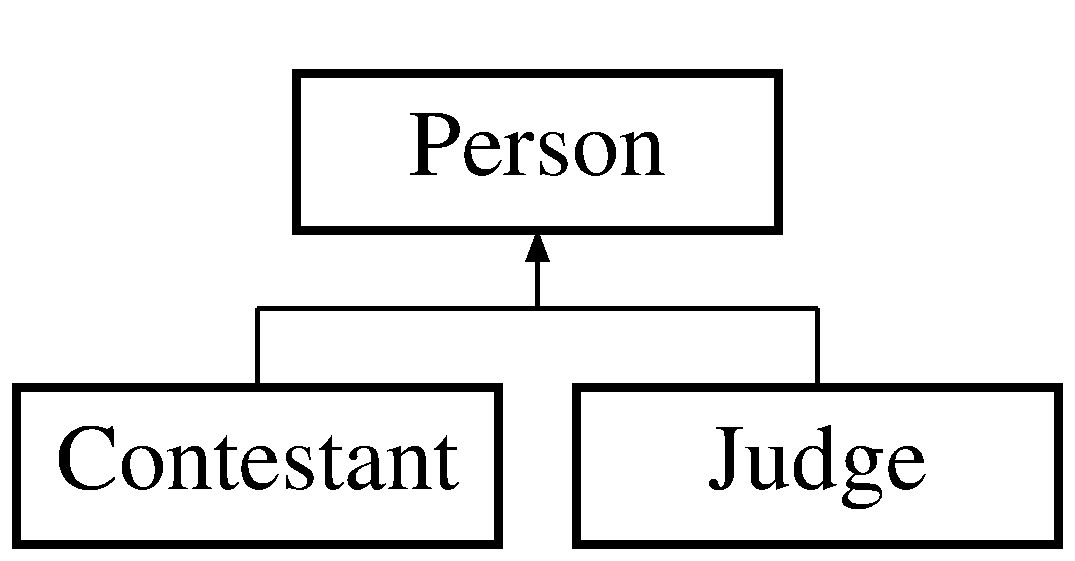
\includegraphics[height=2.000000cm]{class_person}
\end{center}
\end{figure}
\subsection*{Public Member Functions}
\begin{DoxyCompactItemize}
\item 
\mbox{\Hypertarget{class_person_a0397c6f89fafc12e738923f612bc41a3}\label{class_person_a0397c6f89fafc12e738923f612bc41a3}} 
\hyperlink{class_person_a0397c6f89fafc12e738923f612bc41a3}{Person} ()
\begin{DoxyCompactList}\small\item\em \hyperlink{class_person}{Person} Default Contructor. \end{DoxyCompactList}\item 
\hyperlink{class_person_aebae0cd39e3484b689f903fb08c75b45}{Person} (std\+::string name, std\+::string address, unsigned int mobile, \hyperlink{class_calendar}{Calendar} dob, std\+::string specialty)
\begin{DoxyCompactList}\small\item\em \hyperlink{class_person}{Person} Contructor with their id, name, address, mobile phone number, date of birth and specialiy. \end{DoxyCompactList}\item 
std\+::string \hyperlink{class_person_a9db2e2ccfc6cfa0d7979613ec2aaa922}{get\+Name} () const
\begin{DoxyCompactList}\small\item\em Manages to access the \hyperlink{class_person}{Person}\textquotesingle{}s name. \end{DoxyCompactList}\item 
std\+::string \hyperlink{class_person_a5679891e504c02313654d2340953004b}{get\+Address} () const
\begin{DoxyCompactList}\small\item\em Manages to access the \hyperlink{class_person}{Person}\textquotesingle{}s address. \end{DoxyCompactList}\item 
unsigned int \hyperlink{class_person_aac79622064676ce915e2caff620f9af4}{get\+Mobile} () const
\begin{DoxyCompactList}\small\item\em Manages to access the \hyperlink{class_person}{Person}\textquotesingle{}s mobile. \end{DoxyCompactList}\item 
\hyperlink{class_calendar}{Calendar} \hyperlink{class_person_a5ce9adf0875eee7cf702716be85c9d61}{get\+Dob} () const
\begin{DoxyCompactList}\small\item\em Manages to access the \hyperlink{class_person}{Person}\textquotesingle{}s date of birth. \end{DoxyCompactList}\item 
std\+::string \hyperlink{class_person_a9591e789fdcc361389a301d6da3a9376}{get\+Specialty} () const
\begin{DoxyCompactList}\small\item\em Manages to access the \hyperlink{class_person}{Person}\textquotesingle{}s specialiy. \end{DoxyCompactList}\item 
void \hyperlink{class_person_ad6e438f456d3ae6f5b477931c0a6aeba}{set\+Name} (std\+::string name)
\begin{DoxyCompactList}\small\item\em Changes \hyperlink{class_judge}{Judge}\textquotesingle{}s name. \end{DoxyCompactList}\item 
void \hyperlink{class_person_a647fc66d29687250cdba9259e7efe632}{set\+Address} (std\+::string address)
\begin{DoxyCompactList}\small\item\em Changes \hyperlink{class_judge}{Judge}\textquotesingle{}s address. \end{DoxyCompactList}\item 
void \hyperlink{class_person_afa108f8231d33585e5801320a18dbb08}{set\+Mobile} (unsigned int mobile)
\begin{DoxyCompactList}\small\item\em Changes \hyperlink{class_judge}{Judge}\textquotesingle{}s mobile. \end{DoxyCompactList}\item 
void \hyperlink{class_person_afd8a9d5081dc37de47bb97963b984b7e}{set\+Dob} (\hyperlink{class_calendar}{Calendar} dob)
\begin{DoxyCompactList}\small\item\em Changes \hyperlink{class_judge}{Judge}\textquotesingle{}s date of birth. \end{DoxyCompactList}\item 
void \hyperlink{class_person_a1813e3c432b72dbb4b5d7a2686c85c7e}{set\+Specialty} (std\+::string specialty)
\begin{DoxyCompactList}\small\item\em Changes \hyperlink{class_judge}{Judge}\textquotesingle{}s specialty. \end{DoxyCompactList}\item 
unsigned int \hyperlink{class_person_a84de3c2e51ab181bc231a0918faf8fa6}{mobile\+Generator} ()
\begin{DoxyCompactList}\small\item\em Randomly generates a mobile number. \end{DoxyCompactList}\end{DoxyCompactItemize}
\subsection*{Protected Attributes}
\begin{DoxyCompactItemize}
\item 
\mbox{\Hypertarget{class_person_a7594663aadc0de77616506df8a2f4128}\label{class_person_a7594663aadc0de77616506df8a2f4128}} 
std\+::string {\bfseries name}
\item 
\mbox{\Hypertarget{class_person_a348696c2c3209c6740f7c07d1ff6ebd8}\label{class_person_a348696c2c3209c6740f7c07d1ff6ebd8}} 
std\+::string {\bfseries address}
\item 
\mbox{\Hypertarget{class_person_a524573a9dc6aa12b4c6fd2e63bf27352}\label{class_person_a524573a9dc6aa12b4c6fd2e63bf27352}} 
unsigned int {\bfseries mobile}
\item 
\mbox{\Hypertarget{class_person_a639e5be834ff0608c09915be31a5514c}\label{class_person_a639e5be834ff0608c09915be31a5514c}} 
\hyperlink{class_calendar}{Calendar} {\bfseries dob}
\item 
\mbox{\Hypertarget{class_person_a612b37be17477276fec2cf9caaf6aed1}\label{class_person_a612b37be17477276fec2cf9caaf6aed1}} 
std\+::string {\bfseries specialty}
\end{DoxyCompactItemize}


\subsection{Detailed Description}
Project Untitled 

\subsection{Constructor \& Destructor Documentation}
\mbox{\Hypertarget{class_person_aebae0cd39e3484b689f903fb08c75b45}\label{class_person_aebae0cd39e3484b689f903fb08c75b45}} 
\index{Person@{Person}!Person@{Person}}
\index{Person@{Person}!Person@{Person}}
\subsubsection{\texorpdfstring{Person()}{Person()}}
{\footnotesize\ttfamily Person\+::\+Person (\begin{DoxyParamCaption}\item[{std\+::string}]{name,  }\item[{std\+::string}]{address,  }\item[{unsigned int}]{mobile,  }\item[{\hyperlink{class_calendar}{Calendar}}]{dob,  }\item[{std\+::string}]{specialty }\end{DoxyParamCaption})}



\hyperlink{class_person}{Person} Contructor with their id, name, address, mobile phone number, date of birth and specialiy. 


\begin{DoxyParams}{Parameters}
{\em id} & an unsigned integer \\
\hline
{\em name} & a string \\
\hline
{\em address} & a string \\
\hline
{\em mobile} & an unsigned int \\
\hline
{\em dob} & a \hyperlink{class_calendar}{Calendar} Object \\
\hline
{\em specialiy} & a string \\
\hline
\end{DoxyParams}


\subsection{Member Function Documentation}
\mbox{\Hypertarget{class_person_a5679891e504c02313654d2340953004b}\label{class_person_a5679891e504c02313654d2340953004b}} 
\index{Person@{Person}!get\+Address@{get\+Address}}
\index{get\+Address@{get\+Address}!Person@{Person}}
\subsubsection{\texorpdfstring{get\+Address()}{getAddress()}}
{\footnotesize\ttfamily string Person\+::get\+Address (\begin{DoxyParamCaption}{ }\end{DoxyParamCaption}) const}



Manages to access the \hyperlink{class_person}{Person}\textquotesingle{}s address. 

\begin{DoxyReturn}{Returns}
string \hyperlink{class_person}{Person}\textquotesingle{}s adress 
\end{DoxyReturn}
\mbox{\Hypertarget{class_person_a5ce9adf0875eee7cf702716be85c9d61}\label{class_person_a5ce9adf0875eee7cf702716be85c9d61}} 
\index{Person@{Person}!get\+Dob@{get\+Dob}}
\index{get\+Dob@{get\+Dob}!Person@{Person}}
\subsubsection{\texorpdfstring{get\+Dob()}{getDob()}}
{\footnotesize\ttfamily \hyperlink{class_calendar}{Calendar} Person\+::get\+Dob (\begin{DoxyParamCaption}{ }\end{DoxyParamCaption}) const}



Manages to access the \hyperlink{class_person}{Person}\textquotesingle{}s date of birth. 

\begin{DoxyReturn}{Returns}
\hyperlink{class_calendar}{Calendar} Object \hyperlink{class_person}{Person}\textquotesingle{}s date of birth 
\end{DoxyReturn}
\mbox{\Hypertarget{class_person_aac79622064676ce915e2caff620f9af4}\label{class_person_aac79622064676ce915e2caff620f9af4}} 
\index{Person@{Person}!get\+Mobile@{get\+Mobile}}
\index{get\+Mobile@{get\+Mobile}!Person@{Person}}
\subsubsection{\texorpdfstring{get\+Mobile()}{getMobile()}}
{\footnotesize\ttfamily unsigned int Person\+::get\+Mobile (\begin{DoxyParamCaption}{ }\end{DoxyParamCaption}) const}



Manages to access the \hyperlink{class_person}{Person}\textquotesingle{}s mobile. 

\begin{DoxyReturn}{Returns}
unsigned integer \hyperlink{class_person}{Person}\textquotesingle{}s mobile 
\end{DoxyReturn}
\mbox{\Hypertarget{class_person_a9db2e2ccfc6cfa0d7979613ec2aaa922}\label{class_person_a9db2e2ccfc6cfa0d7979613ec2aaa922}} 
\index{Person@{Person}!get\+Name@{get\+Name}}
\index{get\+Name@{get\+Name}!Person@{Person}}
\subsubsection{\texorpdfstring{get\+Name()}{getName()}}
{\footnotesize\ttfamily string Person\+::get\+Name (\begin{DoxyParamCaption}{ }\end{DoxyParamCaption}) const}



Manages to access the \hyperlink{class_person}{Person}\textquotesingle{}s name. 

\begin{DoxyReturn}{Returns}
string \hyperlink{class_person}{Person}\textquotesingle{}s name 
\end{DoxyReturn}
\mbox{\Hypertarget{class_person_a9591e789fdcc361389a301d6da3a9376}\label{class_person_a9591e789fdcc361389a301d6da3a9376}} 
\index{Person@{Person}!get\+Specialty@{get\+Specialty}}
\index{get\+Specialty@{get\+Specialty}!Person@{Person}}
\subsubsection{\texorpdfstring{get\+Specialty()}{getSpecialty()}}
{\footnotesize\ttfamily string Person\+::get\+Specialty (\begin{DoxyParamCaption}{ }\end{DoxyParamCaption}) const}



Manages to access the \hyperlink{class_person}{Person}\textquotesingle{}s specialiy. 

\begin{DoxyReturn}{Returns}
string \hyperlink{class_person}{Person}\textquotesingle{}s specialiy 
\end{DoxyReturn}
\mbox{\Hypertarget{class_person_a84de3c2e51ab181bc231a0918faf8fa6}\label{class_person_a84de3c2e51ab181bc231a0918faf8fa6}} 
\index{Person@{Person}!mobile\+Generator@{mobile\+Generator}}
\index{mobile\+Generator@{mobile\+Generator}!Person@{Person}}
\subsubsection{\texorpdfstring{mobile\+Generator()}{mobileGenerator()}}
{\footnotesize\ttfamily unsigned int Person\+::mobile\+Generator (\begin{DoxyParamCaption}{ }\end{DoxyParamCaption})}



Randomly generates a mobile number. 

\begin{DoxyReturn}{Returns}
unsigned int of the mobile number 
\end{DoxyReturn}
\mbox{\Hypertarget{class_person_a647fc66d29687250cdba9259e7efe632}\label{class_person_a647fc66d29687250cdba9259e7efe632}} 
\index{Person@{Person}!set\+Address@{set\+Address}}
\index{set\+Address@{set\+Address}!Person@{Person}}
\subsubsection{\texorpdfstring{set\+Address()}{setAddress()}}
{\footnotesize\ttfamily void Person\+::set\+Address (\begin{DoxyParamCaption}\item[{std\+::string}]{address }\end{DoxyParamCaption})}



Changes \hyperlink{class_judge}{Judge}\textquotesingle{}s address. 


\begin{DoxyParams}{Parameters}
{\em address} & a string \\
\hline
\end{DoxyParams}
\mbox{\Hypertarget{class_person_afd8a9d5081dc37de47bb97963b984b7e}\label{class_person_afd8a9d5081dc37de47bb97963b984b7e}} 
\index{Person@{Person}!set\+Dob@{set\+Dob}}
\index{set\+Dob@{set\+Dob}!Person@{Person}}
\subsubsection{\texorpdfstring{set\+Dob()}{setDob()}}
{\footnotesize\ttfamily void Person\+::set\+Dob (\begin{DoxyParamCaption}\item[{\hyperlink{class_calendar}{Calendar}}]{dob }\end{DoxyParamCaption})}



Changes \hyperlink{class_judge}{Judge}\textquotesingle{}s date of birth. 


\begin{DoxyParams}{Parameters}
{\em dob} & a \hyperlink{class_calendar}{Calendar} Object \\
\hline
\end{DoxyParams}
\mbox{\Hypertarget{class_person_afa108f8231d33585e5801320a18dbb08}\label{class_person_afa108f8231d33585e5801320a18dbb08}} 
\index{Person@{Person}!set\+Mobile@{set\+Mobile}}
\index{set\+Mobile@{set\+Mobile}!Person@{Person}}
\subsubsection{\texorpdfstring{set\+Mobile()}{setMobile()}}
{\footnotesize\ttfamily void Person\+::set\+Mobile (\begin{DoxyParamCaption}\item[{unsigned int}]{mobile }\end{DoxyParamCaption})}



Changes \hyperlink{class_judge}{Judge}\textquotesingle{}s mobile. 


\begin{DoxyParams}{Parameters}
{\em mobile} & an unsigned integer \\
\hline
\end{DoxyParams}
\mbox{\Hypertarget{class_person_ad6e438f456d3ae6f5b477931c0a6aeba}\label{class_person_ad6e438f456d3ae6f5b477931c0a6aeba}} 
\index{Person@{Person}!set\+Name@{set\+Name}}
\index{set\+Name@{set\+Name}!Person@{Person}}
\subsubsection{\texorpdfstring{set\+Name()}{setName()}}
{\footnotesize\ttfamily void Person\+::set\+Name (\begin{DoxyParamCaption}\item[{std\+::string}]{name }\end{DoxyParamCaption})}



Changes \hyperlink{class_judge}{Judge}\textquotesingle{}s name. 


\begin{DoxyParams}{Parameters}
{\em name} & a string \\
\hline
\end{DoxyParams}
\mbox{\Hypertarget{class_person_a1813e3c432b72dbb4b5d7a2686c85c7e}\label{class_person_a1813e3c432b72dbb4b5d7a2686c85c7e}} 
\index{Person@{Person}!set\+Specialty@{set\+Specialty}}
\index{set\+Specialty@{set\+Specialty}!Person@{Person}}
\subsubsection{\texorpdfstring{set\+Specialty()}{setSpecialty()}}
{\footnotesize\ttfamily void Person\+::set\+Specialty (\begin{DoxyParamCaption}\item[{std\+::string}]{specialty }\end{DoxyParamCaption})}



Changes \hyperlink{class_judge}{Judge}\textquotesingle{}s specialty. 


\begin{DoxyParams}{Parameters}
{\em specialty} & a string \\
\hline
\end{DoxyParams}


The documentation for this class was generated from the following files\+:\begin{DoxyCompactItemize}
\item 
Person.\+h\item 
Person.\+cpp\end{DoxyCompactItemize}

\hypertarget{class_phase}{}\section{Phase Class Reference}
\label{class_phase}\index{Phase@{Phase}}


{\ttfamily \#include $<$Phase.\+h$>$}

Inheritance diagram for Phase\+:\begin{figure}[H]
\begin{center}
\leavevmode
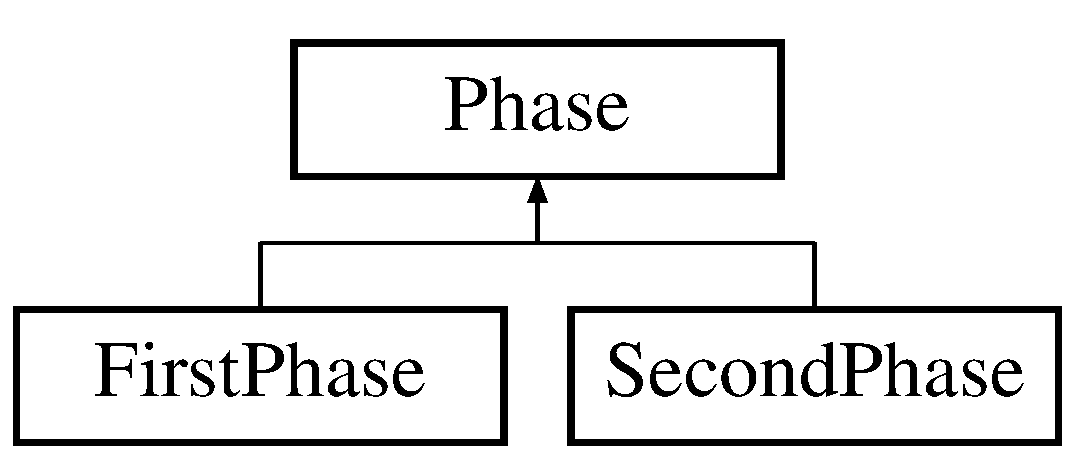
\includegraphics[height=2.000000cm]{class_phase}
\end{center}
\end{figure}
\subsection*{Public Member Functions}
\begin{DoxyCompactItemize}
\item 
\mbox{\Hypertarget{class_phase_a3760262f782f336aa55c1f14266fc455}\label{class_phase_a3760262f782f336aa55c1f14266fc455}} 
\hyperlink{class_phase_a3760262f782f336aa55c1f14266fc455}{Phase} ()
\begin{DoxyCompactList}\small\item\em \hyperlink{class_phase}{Phase} default constructor. \end{DoxyCompactList}\item 
\mbox{\Hypertarget{class_phase_ad66fc793040c3e37c2c3e954edfc627d}\label{class_phase_ad66fc793040c3e37c2c3e954edfc627d}} 
virtual \hyperlink{class_phase_ad66fc793040c3e37c2c3e954edfc627d}{$\sim$\+Phase} ()
\begin{DoxyCompactList}\small\item\em \hyperlink{class_phase}{Phase} deconstructor. \end{DoxyCompactList}\item 
\hyperlink{class_phase_a19be92bd99171dcd6f202aa414941df8}{Phase} (unsigned int audition\+Id, std\+::vector$<$ unsigned int $>$ final\+\_\+grade, std\+::vector$<$ unsigned int $>$ judge1, std\+::vector$<$ unsigned int $>$ judge2, std\+::vector$<$ unsigned int $>$ chief\+Judge, std\+::vector$<$ unsigned int $>$ contestants)
\begin{DoxyCompactList}\small\item\em \hyperlink{class_phase}{Phase} default constructor with their audition\+ID, final grade, evaluation from the judges and the id of the contestants. \end{DoxyCompactList}\item 
\hyperlink{class_phase_ad0e5ebffc33f2127e147b0330e72efd5}{Phase} (std\+::string textline)
\begin{DoxyCompactList}\small\item\em \hyperlink{class_phase}{Phase} constructor by reading a line from the file. \end{DoxyCompactList}\item 
unsigned int \hyperlink{class_phase_a7d5b0ced6ad5d523cace56f9122b0af2}{get\+Audition\+Id} () const
\begin{DoxyCompactList}\small\item\em Manages to get the audition\textquotesingle{}s id. \end{DoxyCompactList}\item 
std\+::vector$<$ double $>$ \hyperlink{class_phase_acc55a56cbaec90a2972cb78ad8ce085c}{get\+Final\+Grade} () const
\begin{DoxyCompactList}\small\item\em Manages access all the final grades from the contestants of a certain phase. \end{DoxyCompactList}\item 
std\+::vector$<$ unsigned int $>$ \hyperlink{class_phase_aa705f5aa86b20627a115034ed9881246}{get\+Judge1} () const
\begin{DoxyCompactList}\small\item\em Manages access the grades the first judge gave to all contestants of a certain phase. \end{DoxyCompactList}\item 
std\+::vector$<$ unsigned int $>$ \hyperlink{class_phase_ac8f4328b114a36e3296ee2f4e9fd06e8}{get\+Judge2} () const
\begin{DoxyCompactList}\small\item\em Manages access the grades the second judge gave to all contestants of a certain phase. \end{DoxyCompactList}\item 
std\+::vector$<$ unsigned int $>$ \hyperlink{class_phase_a1c251350327ab06f2cc8bb8f1331d370}{get\+Chief\+Judge} () const
\begin{DoxyCompactList}\small\item\em Manages access the grades the reposible judge gave to all contestants of a certain phase. \end{DoxyCompactList}\item 
std\+::vector$<$ unsigned int $>$ \hyperlink{class_phase_a670856408ac3d956d30e371dd69fbf13}{get\+Contestants} () const
\begin{DoxyCompactList}\small\item\em Manages access the id of all contestants of a certain phase. \end{DoxyCompactList}\item 
void \hyperlink{class_phase_af2bc70b0e24880d38e42f37ef31164ac}{set\+Audition\+Id} (unsigned int audition\+Id)
\begin{DoxyCompactList}\small\item\em Changes the id of an audition. \end{DoxyCompactList}\item 
void \hyperlink{class_phase_a3a08956302c65b5ccea41521059a787c}{set\+Contestants} (std\+::vector$<$ unsigned int $>$ contestants)
\begin{DoxyCompactList}\small\item\em Changes the id of all contestants. \end{DoxyCompactList}\item 
\mbox{\Hypertarget{class_phase_af57b6ad20a1b4790f55e97b8f68fdd7c}\label{class_phase_af57b6ad20a1b4790f55e97b8f68fdd7c}} 
void \hyperlink{class_phase_af57b6ad20a1b4790f55e97b8f68fdd7c}{evaluate} ()
\begin{DoxyCompactList}\small\item\em Randomly assigns the the individual grades of each judges to all contestants. \end{DoxyCompactList}\item 
\mbox{\Hypertarget{class_phase_a672ed9cf455ca8dbf89fc56687d455b3}\label{class_phase_a672ed9cf455ca8dbf89fc56687d455b3}} 
virtual void \hyperlink{class_phase_a672ed9cf455ca8dbf89fc56687d455b3}{overall\+Grading} ()=0
\begin{DoxyCompactList}\small\item\em Virtual function to grade all contestants. \end{DoxyCompactList}\end{DoxyCompactItemize}
\subsection*{Protected Attributes}
\begin{DoxyCompactItemize}
\item 
\mbox{\Hypertarget{class_phase_a3e576bda9c8be6db31bf3c46ab1284ca}\label{class_phase_a3e576bda9c8be6db31bf3c46ab1284ca}} 
unsigned int {\bfseries audition\+Id}
\item 
\mbox{\Hypertarget{class_phase_a44fede0ef598b2689aef0ecd213ac156}\label{class_phase_a44fede0ef598b2689aef0ecd213ac156}} 
std\+::vector$<$ double $>$ {\bfseries final\+Grade}
\item 
\mbox{\Hypertarget{class_phase_abd94426c3e881880e3fea3d5d70310b9}\label{class_phase_abd94426c3e881880e3fea3d5d70310b9}} 
std\+::vector$<$ unsigned int $>$ {\bfseries judge1}
\item 
\mbox{\Hypertarget{class_phase_a658128a2fbbe3b9bc4fb672bf851f45c}\label{class_phase_a658128a2fbbe3b9bc4fb672bf851f45c}} 
std\+::vector$<$ unsigned int $>$ {\bfseries judge2}
\item 
\mbox{\Hypertarget{class_phase_ad6179ca6a93733eb072e2808c357a2d4}\label{class_phase_ad6179ca6a93733eb072e2808c357a2d4}} 
std\+::vector$<$ unsigned int $>$ {\bfseries chief\+Judge}
\item 
\mbox{\Hypertarget{class_phase_ae0511c17f00d8856298e23a9288ba698}\label{class_phase_ae0511c17f00d8856298e23a9288ba698}} 
std\+::vector$<$ unsigned int $>$ {\bfseries contestants}
\end{DoxyCompactItemize}


\subsection{Detailed Description}
Project Untitled 

\subsection{Constructor \& Destructor Documentation}
\mbox{\Hypertarget{class_phase_a19be92bd99171dcd6f202aa414941df8}\label{class_phase_a19be92bd99171dcd6f202aa414941df8}} 
\index{Phase@{Phase}!Phase@{Phase}}
\index{Phase@{Phase}!Phase@{Phase}}
\subsubsection{\texorpdfstring{Phase()}{Phase()}\hspace{0.1cm}{\footnotesize\ttfamily [1/2]}}
{\footnotesize\ttfamily Phase\+::\+Phase (\begin{DoxyParamCaption}\item[{unsigned int}]{audition\+Id,  }\item[{std\+::vector$<$ unsigned int $>$}]{final\+\_\+grade,  }\item[{std\+::vector$<$ unsigned int $>$}]{judge1,  }\item[{std\+::vector$<$ unsigned int $>$}]{judge2,  }\item[{std\+::vector$<$ unsigned int $>$}]{chief\+Judge,  }\item[{std\+::vector$<$ unsigned int $>$}]{contestants }\end{DoxyParamCaption})}



\hyperlink{class_phase}{Phase} default constructor with their audition\+ID, final grade, evaluation from the judges and the id of the contestants. 


\begin{DoxyParams}{Parameters}
{\em audition\+ID} & an unsigned integer \\
\hline
{\em final\+\_\+grade} & a vector of unsigned integers \\
\hline
{\em ev1} & a vector of unsigned integers \\
\hline
{\em ev2} & a vector of unsigned integers \\
\hline
{\em ld} & a vector of unsigned integers \\
\hline
{\em contestants} & a vector of unsigned integers \\
\hline
\end{DoxyParams}
\mbox{\Hypertarget{class_phase_ad0e5ebffc33f2127e147b0330e72efd5}\label{class_phase_ad0e5ebffc33f2127e147b0330e72efd5}} 
\index{Phase@{Phase}!Phase@{Phase}}
\index{Phase@{Phase}!Phase@{Phase}}
\subsubsection{\texorpdfstring{Phase()}{Phase()}\hspace{0.1cm}{\footnotesize\ttfamily [2/2]}}
{\footnotesize\ttfamily Phase\+::\+Phase (\begin{DoxyParamCaption}\item[{std\+::string}]{textline }\end{DoxyParamCaption})}



\hyperlink{class_phase}{Phase} constructor by reading a line from the file. 


\begin{DoxyParams}{Parameters}
{\em text\+Line} & a string \\
\hline
\end{DoxyParams}


\subsection{Member Function Documentation}
\mbox{\Hypertarget{class_phase_a7d5b0ced6ad5d523cace56f9122b0af2}\label{class_phase_a7d5b0ced6ad5d523cace56f9122b0af2}} 
\index{Phase@{Phase}!get\+Audition\+Id@{get\+Audition\+Id}}
\index{get\+Audition\+Id@{get\+Audition\+Id}!Phase@{Phase}}
\subsubsection{\texorpdfstring{get\+Audition\+Id()}{getAuditionId()}}
{\footnotesize\ttfamily unsigned int Phase\+::get\+Audition\+Id (\begin{DoxyParamCaption}{ }\end{DoxyParamCaption}) const}



Manages to get the audition\textquotesingle{}s id. 

\begin{DoxyReturn}{Returns}
unsigned integer 
\end{DoxyReturn}
\mbox{\Hypertarget{class_phase_a1c251350327ab06f2cc8bb8f1331d370}\label{class_phase_a1c251350327ab06f2cc8bb8f1331d370}} 
\index{Phase@{Phase}!get\+Chief\+Judge@{get\+Chief\+Judge}}
\index{get\+Chief\+Judge@{get\+Chief\+Judge}!Phase@{Phase}}
\subsubsection{\texorpdfstring{get\+Chief\+Judge()}{getChiefJudge()}}
{\footnotesize\ttfamily vector$<$ unsigned int $>$ Phase\+::get\+Chief\+Judge (\begin{DoxyParamCaption}{ }\end{DoxyParamCaption}) const}



Manages access the grades the reposible judge gave to all contestants of a certain phase. 

\begin{DoxyReturn}{Returns}
vector of unsigned integers the grade of the resposible judge 
\end{DoxyReturn}
\mbox{\Hypertarget{class_phase_a670856408ac3d956d30e371dd69fbf13}\label{class_phase_a670856408ac3d956d30e371dd69fbf13}} 
\index{Phase@{Phase}!get\+Contestants@{get\+Contestants}}
\index{get\+Contestants@{get\+Contestants}!Phase@{Phase}}
\subsubsection{\texorpdfstring{get\+Contestants()}{getContestants()}}
{\footnotesize\ttfamily vector$<$ unsigned int $>$ Phase\+::get\+Contestants (\begin{DoxyParamCaption}{ }\end{DoxyParamCaption}) const}



Manages access the id of all contestants of a certain phase. 

\begin{DoxyReturn}{Returns}
vector of unsigned integers 
\end{DoxyReturn}
\mbox{\Hypertarget{class_phase_acc55a56cbaec90a2972cb78ad8ce085c}\label{class_phase_acc55a56cbaec90a2972cb78ad8ce085c}} 
\index{Phase@{Phase}!get\+Final\+Grade@{get\+Final\+Grade}}
\index{get\+Final\+Grade@{get\+Final\+Grade}!Phase@{Phase}}
\subsubsection{\texorpdfstring{get\+Final\+Grade()}{getFinalGrade()}}
{\footnotesize\ttfamily vector$<$ double $>$ Phase\+::get\+Final\+Grade (\begin{DoxyParamCaption}{ }\end{DoxyParamCaption}) const}



Manages access all the final grades from the contestants of a certain phase. 

\begin{DoxyReturn}{Returns}
vector of doubles the final grade 
\end{DoxyReturn}
\mbox{\Hypertarget{class_phase_aa705f5aa86b20627a115034ed9881246}\label{class_phase_aa705f5aa86b20627a115034ed9881246}} 
\index{Phase@{Phase}!get\+Judge1@{get\+Judge1}}
\index{get\+Judge1@{get\+Judge1}!Phase@{Phase}}
\subsubsection{\texorpdfstring{get\+Judge1()}{getJudge1()}}
{\footnotesize\ttfamily vector$<$ unsigned int $>$ Phase\+::get\+Judge1 (\begin{DoxyParamCaption}{ }\end{DoxyParamCaption}) const}



Manages access the grades the first judge gave to all contestants of a certain phase. 

\begin{DoxyReturn}{Returns}
vector of unsigned integers the grade of the first judge 
\end{DoxyReturn}
\mbox{\Hypertarget{class_phase_ac8f4328b114a36e3296ee2f4e9fd06e8}\label{class_phase_ac8f4328b114a36e3296ee2f4e9fd06e8}} 
\index{Phase@{Phase}!get\+Judge2@{get\+Judge2}}
\index{get\+Judge2@{get\+Judge2}!Phase@{Phase}}
\subsubsection{\texorpdfstring{get\+Judge2()}{getJudge2()}}
{\footnotesize\ttfamily vector$<$ unsigned int $>$ Phase\+::get\+Judge2 (\begin{DoxyParamCaption}{ }\end{DoxyParamCaption}) const}



Manages access the grades the second judge gave to all contestants of a certain phase. 

\begin{DoxyReturn}{Returns}
vector of unsigned integers the grade of the second judge 
\end{DoxyReturn}
\mbox{\Hypertarget{class_phase_af2bc70b0e24880d38e42f37ef31164ac}\label{class_phase_af2bc70b0e24880d38e42f37ef31164ac}} 
\index{Phase@{Phase}!set\+Audition\+Id@{set\+Audition\+Id}}
\index{set\+Audition\+Id@{set\+Audition\+Id}!Phase@{Phase}}
\subsubsection{\texorpdfstring{set\+Audition\+Id()}{setAuditionId()}}
{\footnotesize\ttfamily void Phase\+::set\+Audition\+Id (\begin{DoxyParamCaption}\item[{unsigned int}]{audition\+Id }\end{DoxyParamCaption})}



Changes the id of an audition. 


\begin{DoxyParams}{Parameters}
{\em audition\+Id} & unsigned integer \\
\hline
\end{DoxyParams}
\mbox{\Hypertarget{class_phase_a3a08956302c65b5ccea41521059a787c}\label{class_phase_a3a08956302c65b5ccea41521059a787c}} 
\index{Phase@{Phase}!set\+Contestants@{set\+Contestants}}
\index{set\+Contestants@{set\+Contestants}!Phase@{Phase}}
\subsubsection{\texorpdfstring{set\+Contestants()}{setContestants()}}
{\footnotesize\ttfamily void Phase\+::set\+Contestants (\begin{DoxyParamCaption}\item[{std\+::vector$<$ unsigned int $>$}]{contestants }\end{DoxyParamCaption})}



Changes the id of all contestants. 


\begin{DoxyParams}{Parameters}
{\em contestants} & unsigned integer \\
\hline
\end{DoxyParams}


The documentation for this class was generated from the following files\+:\begin{DoxyCompactItemize}
\item 
Phase.\+h\item 
Phase.\+cpp\end{DoxyCompactItemize}

\hypertarget{class_second_phase}{}\section{Second\+Phase Class Reference}
\label{class_second_phase}\index{Second\+Phase@{Second\+Phase}}


{\ttfamily \#include $<$Second\+Phase.\+h$>$}

Inheritance diagram for Second\+Phase\+:\begin{figure}[H]
\begin{center}
\leavevmode
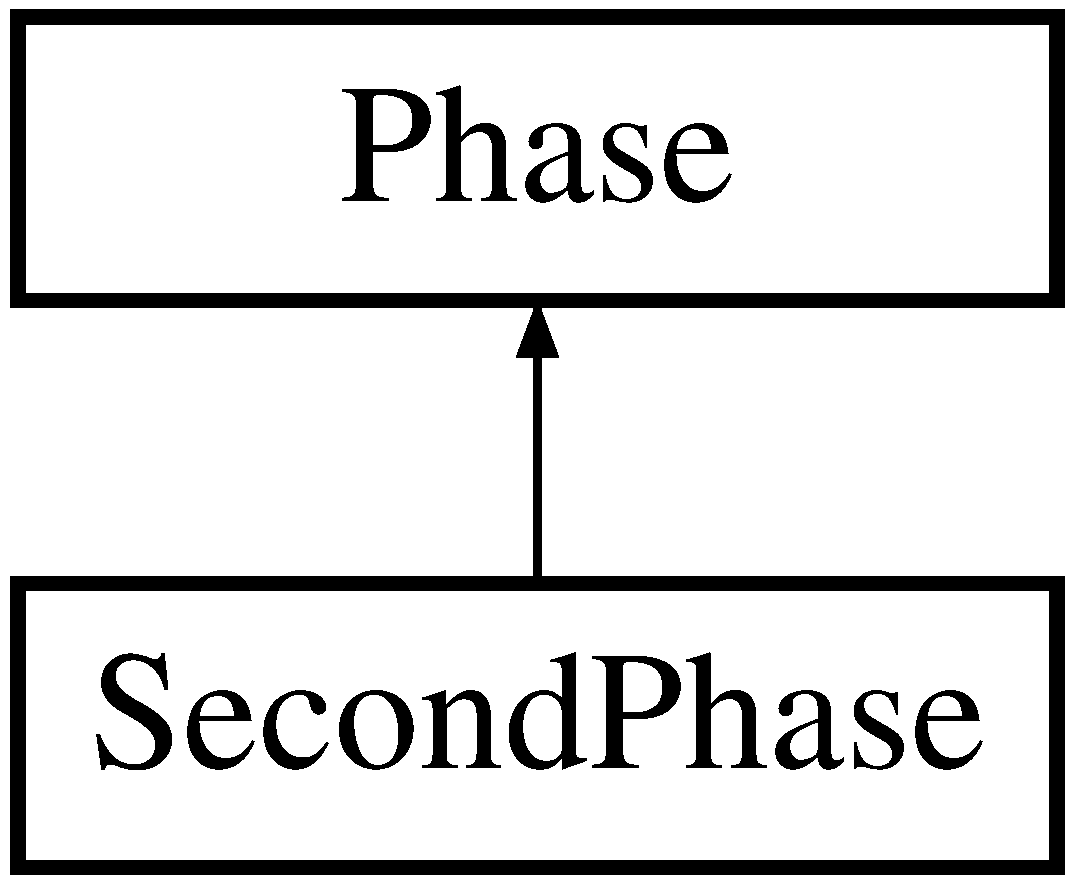
\includegraphics[height=2.000000cm]{class_second_phase}
\end{center}
\end{figure}
\subsection*{Public Member Functions}
\begin{DoxyCompactItemize}
\item 
\mbox{\Hypertarget{class_second_phase_ae8acf3524c58a688b2ef939d33c0cb77}\label{class_second_phase_ae8acf3524c58a688b2ef939d33c0cb77}} 
\hyperlink{class_second_phase_ae8acf3524c58a688b2ef939d33c0cb77}{Second\+Phase} ()
\begin{DoxyCompactList}\small\item\em Second \hyperlink{class_phase}{Phase} default constructor. \end{DoxyCompactList}\item 
\mbox{\Hypertarget{class_second_phase_aa5277652125f6700334abd7619b8f9e6}\label{class_second_phase_aa5277652125f6700334abd7619b8f9e6}} 
\hyperlink{class_second_phase_aa5277652125f6700334abd7619b8f9e6}{$\sim$\+Second\+Phase} ()
\begin{DoxyCompactList}\small\item\em Second \hyperlink{class_phase}{Phase} deconstructor. \end{DoxyCompactList}\item 
\hyperlink{class_second_phase_ac22a81240fb312f9ecdb1d8edb72ea9d}{Second\+Phase} (unsigned int audition\+Id, std\+::vector$<$ unsigned int $>$ final\+\_\+grade, std\+::vector$<$ unsigned int $>$ ev1, std\+::vector$<$ unsigned int $>$ ev2, std\+::vector$<$ unsigned int $>$ ld, std\+::vector$<$ unsigned int $>$ contestants)
\begin{DoxyCompactList}\small\item\em Second \hyperlink{class_phase}{Phase} default constructor with their audition\+ID, final grade, evaluation from the judges and the id of the contestants. \end{DoxyCompactList}\item 
\hyperlink{class_second_phase_ac65ce65f9908610e35fee1635be6d8af}{Second\+Phase} (std\+::string text\+Line)
\begin{DoxyCompactList}\small\item\em Second \hyperlink{class_phase}{Phase} constructor by reading a line from the file. \end{DoxyCompactList}\item 
\mbox{\Hypertarget{class_second_phase_a54ab71dc4d4d6ffb38792767eeded188}\label{class_second_phase_a54ab71dc4d4d6ffb38792767eeded188}} 
virtual void \hyperlink{class_second_phase_a54ab71dc4d4d6ffb38792767eeded188}{overall\+Grading} ()
\begin{DoxyCompactList}\small\item\em Grades all contestants from the second phase. \end{DoxyCompactList}\end{DoxyCompactItemize}
\subsection*{Friends}
\begin{DoxyCompactItemize}
\item 
std\+::ostream \& \hyperlink{class_second_phase_a8b0fca2bfcb7697b3e998ea39ef2f5cb}{operator$<$$<$} (std\+::ostream \&os, const \hyperlink{class_second_phase}{Second\+Phase} \&second\+Phase)
\end{DoxyCompactItemize}
\subsection*{Additional Inherited Members}


\subsection{Detailed Description}
Project Untitled 

\subsection{Constructor \& Destructor Documentation}
\mbox{\Hypertarget{class_second_phase_ac22a81240fb312f9ecdb1d8edb72ea9d}\label{class_second_phase_ac22a81240fb312f9ecdb1d8edb72ea9d}} 
\index{Second\+Phase@{Second\+Phase}!Second\+Phase@{Second\+Phase}}
\index{Second\+Phase@{Second\+Phase}!Second\+Phase@{Second\+Phase}}
\subsubsection{\texorpdfstring{Second\+Phase()}{SecondPhase()}\hspace{0.1cm}{\footnotesize\ttfamily [1/2]}}
{\footnotesize\ttfamily Second\+Phase\+::\+Second\+Phase (\begin{DoxyParamCaption}\item[{unsigned int}]{audition\+Id,  }\item[{std\+::vector$<$ unsigned int $>$}]{final\+\_\+grade,  }\item[{std\+::vector$<$ unsigned int $>$}]{ev1,  }\item[{std\+::vector$<$ unsigned int $>$}]{ev2,  }\item[{std\+::vector$<$ unsigned int $>$}]{ld,  }\item[{std\+::vector$<$ unsigned int $>$}]{contestants }\end{DoxyParamCaption})}



Second \hyperlink{class_phase}{Phase} default constructor with their audition\+ID, final grade, evaluation from the judges and the id of the contestants. 


\begin{DoxyParams}{Parameters}
{\em audition\+ID} & an unsigned integer \\
\hline
{\em final\+\_\+grade} & a vector of unsigned integers \\
\hline
{\em ev1} & a vector of unsigned integers \\
\hline
{\em ev2} & a vector of unsigned integers \\
\hline
{\em ld} & a vector of unsigned integers \\
\hline
{\em contestants} & a vector of unsigned integers \\
\hline
\end{DoxyParams}
\mbox{\Hypertarget{class_second_phase_ac65ce65f9908610e35fee1635be6d8af}\label{class_second_phase_ac65ce65f9908610e35fee1635be6d8af}} 
\index{Second\+Phase@{Second\+Phase}!Second\+Phase@{Second\+Phase}}
\index{Second\+Phase@{Second\+Phase}!Second\+Phase@{Second\+Phase}}
\subsubsection{\texorpdfstring{Second\+Phase()}{SecondPhase()}\hspace{0.1cm}{\footnotesize\ttfamily [2/2]}}
{\footnotesize\ttfamily Second\+Phase\+::\+Second\+Phase (\begin{DoxyParamCaption}\item[{std\+::string}]{text\+Line }\end{DoxyParamCaption})}



Second \hyperlink{class_phase}{Phase} constructor by reading a line from the file. 


\begin{DoxyParams}{Parameters}
{\em text\+Line} & a string \\
\hline
\end{DoxyParams}


\subsection{Friends And Related Function Documentation}
\mbox{\Hypertarget{class_second_phase_a8b0fca2bfcb7697b3e998ea39ef2f5cb}\label{class_second_phase_a8b0fca2bfcb7697b3e998ea39ef2f5cb}} 
\index{Second\+Phase@{Second\+Phase}!operator$<$$<$@{operator$<$$<$}}
\index{operator$<$$<$@{operator$<$$<$}!Second\+Phase@{Second\+Phase}}
\subsubsection{\texorpdfstring{operator$<$$<$}{operator<<}}
{\footnotesize\ttfamily std\+::ostream\& operator$<$$<$ (\begin{DoxyParamCaption}\item[{std\+::ostream \&}]{os,  }\item[{const \hyperlink{class_second_phase}{Second\+Phase} \&}]{second\+Phase }\end{DoxyParamCaption})\hspace{0.3cm}{\ttfamily [friend]}}

Operator \char`\"{}$<$$<$\char`\"{} is overloaded to output the information about the Second \hyperlink{class_phase}{Phase} into a file 
\begin{DoxyParams}{Parameters}
{\em os} & an Outstream Object \\
\hline
{\em second\+Phase} & a constant \hyperlink{class_second_phase}{Second\+Phase} reference \\
\hline
\end{DoxyParams}
\begin{DoxyReturn}{Returns}
the information of the Second \hyperlink{class_phase}{Phase} in a specific format into a file 
\end{DoxyReturn}


The documentation for this class was generated from the following files\+:\begin{DoxyCompactItemize}
\item 
Second\+Phase.\+h\item 
Second\+Phase.\+cpp\end{DoxyCompactItemize}

\hypertarget{class_specialty_not_available}{}\section{Specialty\+Not\+Available Class Reference}
\label{class_specialty_not_available}\index{Specialty\+Not\+Available@{Specialty\+Not\+Available}}
\subsection*{Public Member Functions}
\begin{DoxyCompactItemize}
\item 
\mbox{\Hypertarget{class_specialty_not_available_a1f5f874d6227ffd1083d2f07657ca8f6}\label{class_specialty_not_available_a1f5f874d6227ffd1083d2f07657ca8f6}} 
{\bfseries Specialty\+Not\+Available} (string specialty)
\item 
string \hyperlink{class_specialty_not_available_aeb467ae8d75b1bc7b937fd1683deff6e}{get\+Specialty} () const
\begin{DoxyCompactList}\small\item\em Manages to get the id of the specialty that is not available. \end{DoxyCompactList}\end{DoxyCompactItemize}


\subsection{Member Function Documentation}
\mbox{\Hypertarget{class_specialty_not_available_aeb467ae8d75b1bc7b937fd1683deff6e}\label{class_specialty_not_available_aeb467ae8d75b1bc7b937fd1683deff6e}} 
\index{Specialty\+Not\+Available@{Specialty\+Not\+Available}!get\+Specialty@{get\+Specialty}}
\index{get\+Specialty@{get\+Specialty}!Specialty\+Not\+Available@{Specialty\+Not\+Available}}
\subsubsection{\texorpdfstring{get\+Specialty()}{getSpecialty()}}
{\footnotesize\ttfamily string Specialty\+Not\+Available\+::get\+Specialty (\begin{DoxyParamCaption}{ }\end{DoxyParamCaption}) const\hspace{0.3cm}{\ttfamily [inline]}}



Manages to get the id of the specialty that is not available. 

\begin{DoxyReturn}{Returns}
string of the speciality that is not available 
\end{DoxyReturn}


The documentation for this class was generated from the following file\+:\begin{DoxyCompactItemize}
\item 
Exception\+Hand.\+h\end{DoxyCompactItemize}

%--- End generated contents ---

% Index
\backmatter
\newpage
\phantomsection
\clearemptydoublepage
\addcontentsline{toc}{chapter}{Index}
\printindex

\end{document}
